\documentclass[aspectratio=169,c]{beamer}
\usetheme{default}
\usecolortheme{dove}
\setbeamertemplate{navigation symbols}{}

% ── Fonts and microtypography ──────────────────────────────────
\usepackage{lmodern}
\usepackage{microtype}

% ── Color palette ──────────────────────────────────────────────
\definecolor{primary}{RGB}{23,63,95}
\definecolor{medgray}{RGB}{140,140,140}

\setbeamercolor{title}{fg=primary}
\setbeamercolor{subtitle}{fg=medgray}
\setbeamercolor{frametitle}{fg=primary}
\setbeamercolor{structure}{fg=primary}

% ── Frame titles (centered, colored) ──────────────────────────
\setbeamertemplate{frametitle}[default][center]

% ── Title page ─────────────────────────────────────────────────
\setbeamertemplate{title page}{
  \vfill
  \centering
  {\color{primary!40}\rule{0.45\textwidth}{0.4pt}}\\[1.5em]
  {\usebeamerfont{title}\usebeamercolor[fg]{title}\inserttitle}\\[0.8em]
  {\usebeamerfont{subtitle}\usebeamercolor[fg]{subtitle}\insertsubtitle}\\[1.5em]
  {\color{primary!40}\rule{0.45\textwidth}{0.4pt}}
  \vfill
}

% ── Footline ───────────────────────────────────────────────────
\newcommand{\defaultfootline}{%
  \setbeamertemplate{footline}{%
    \hfill{\color{medgray}\scriptsize\insertframenumber\kern14pt}\vskip6pt%
  }%
}
\defaultfootline

\newcommand{\hideframenumber}{%
  \setbeamertemplate{footline}{}%
  \addtocounter{framenumber}{-1}%
}
\newcommand{\showframenumber}{\defaultfootline}

% ── Section and subsection pages ───────────────────────────────
\setbeamertemplate{section page}{
  \centering
  \vfill
  {\color{primary!40}\rule{0.35\textwidth}{0.4pt}}\\[1.2em]
  {\LARGE\bfseries\color{primary}\thesection.~\insertsection}\\[1.2em]
  {\color{primary!40}\rule{0.35\textwidth}{0.4pt}}
  \vfill
}
\setbeamertemplate{subsection page}{
  \centering
  \vfill
  {\normalsize\color{medgray}\thesection.~\insertsection}\\[1em]
  {\color{primary!30}\rule{0.25\textwidth}{0.3pt}}\\[1em]
  {\Large\bfseries\color{primary}\thesection.\thesubsection~\insertsubsection}
  \vfill
}

% ── Table of contents ──────────────────────────────────────────
\setbeamertemplate{section in toc}{%
  \inserttocsectionnumber.~\inserttocsection\par%
}

% ── Spacing ────────────────────────────────────────────────────
\setbeamertemplate{itemize/enumerate body begin}{\setlength\itemsep{6pt}}
\setbeamertemplate{itemize/enumerate subbody begin}{\setlength\itemsep{4pt}}
\renewcommand{\arraystretch}{1.25}

% ── Packages ───────────────────────────────────────────────────
\usepackage{graphicx}
\usepackage{amsmath}
\usepackage{booktabs}

\title{Local Projections: Natural Disaster Shocks and GDP}
\subtitle{\texttt{lp\_gdp\_shocks.R}}
\date{}

\begin{document}

\begin{frame}
\titlepage
\end{frame}

\begin{frame}{Outline}
\small
\tableofcontents[hideallsubsections]
\end{frame}

\begin{frame}{Key Findings}
\begin{enumerate}
  \item Cyclone shocks reduce GDP per capita by \textbf{2--4\%} over 5--10 years
  \item With standard year FE, post-1990 effects appear larger --- but this is an \textbf{artifact of control group composition}
  \item 142/182 countries never experience cyclones; they are concentrated in \textbf{Europe and Africa}, while treated countries are in the \textbf{Americas and Asia}
  \item With \textbf{region$\times$year FE}, the pre/post-1990 divergence \textbf{disappears}
\end{enumerate}
\end{frame}

% ===============================================================
\section{Data and Shocks}
% ===============================================================

{\hideframenumber
\begin{frame}
\sectionpage
\end{frame}
\showframenumber}

\begin{frame}{Data Sources}
\begin{itemize}
  \item \textbf{GDP}: Penn World Tables --- log real GDP per capita, growth rates
  \item \textbf{Cyclones}: IBTrACS --- max wind speed, cumulative energy, landfalls
  \item Joined on (country, year); wind converted from knots to m/s
  \item Sample: 1969--2014, balanced country--year panel (182 countries)
\end{itemize}
\end{frame}

\begin{frame}{Shock Definition}
Three cyclone measures, each used in two forms:
\bigskip
\begin{enumerate}
  \item \textbf{Max Wind Speed} --- peak sustained wind in a country--year
  \item \textbf{Cyclone Energy} --- cumulative energy of all storms
  \item \textbf{Landfalls} --- number of cyclone landfalls
\end{enumerate}
\bigskip
\begin{description}
  \item[Binary] $= 1$ if above global 95th percentile (1970--2014)
  \item[Continuous] standardized by SD (among exposed country--years)
\end{description}
\end{frame}

\begin{frame}{Shock Events Over Time}
\centering
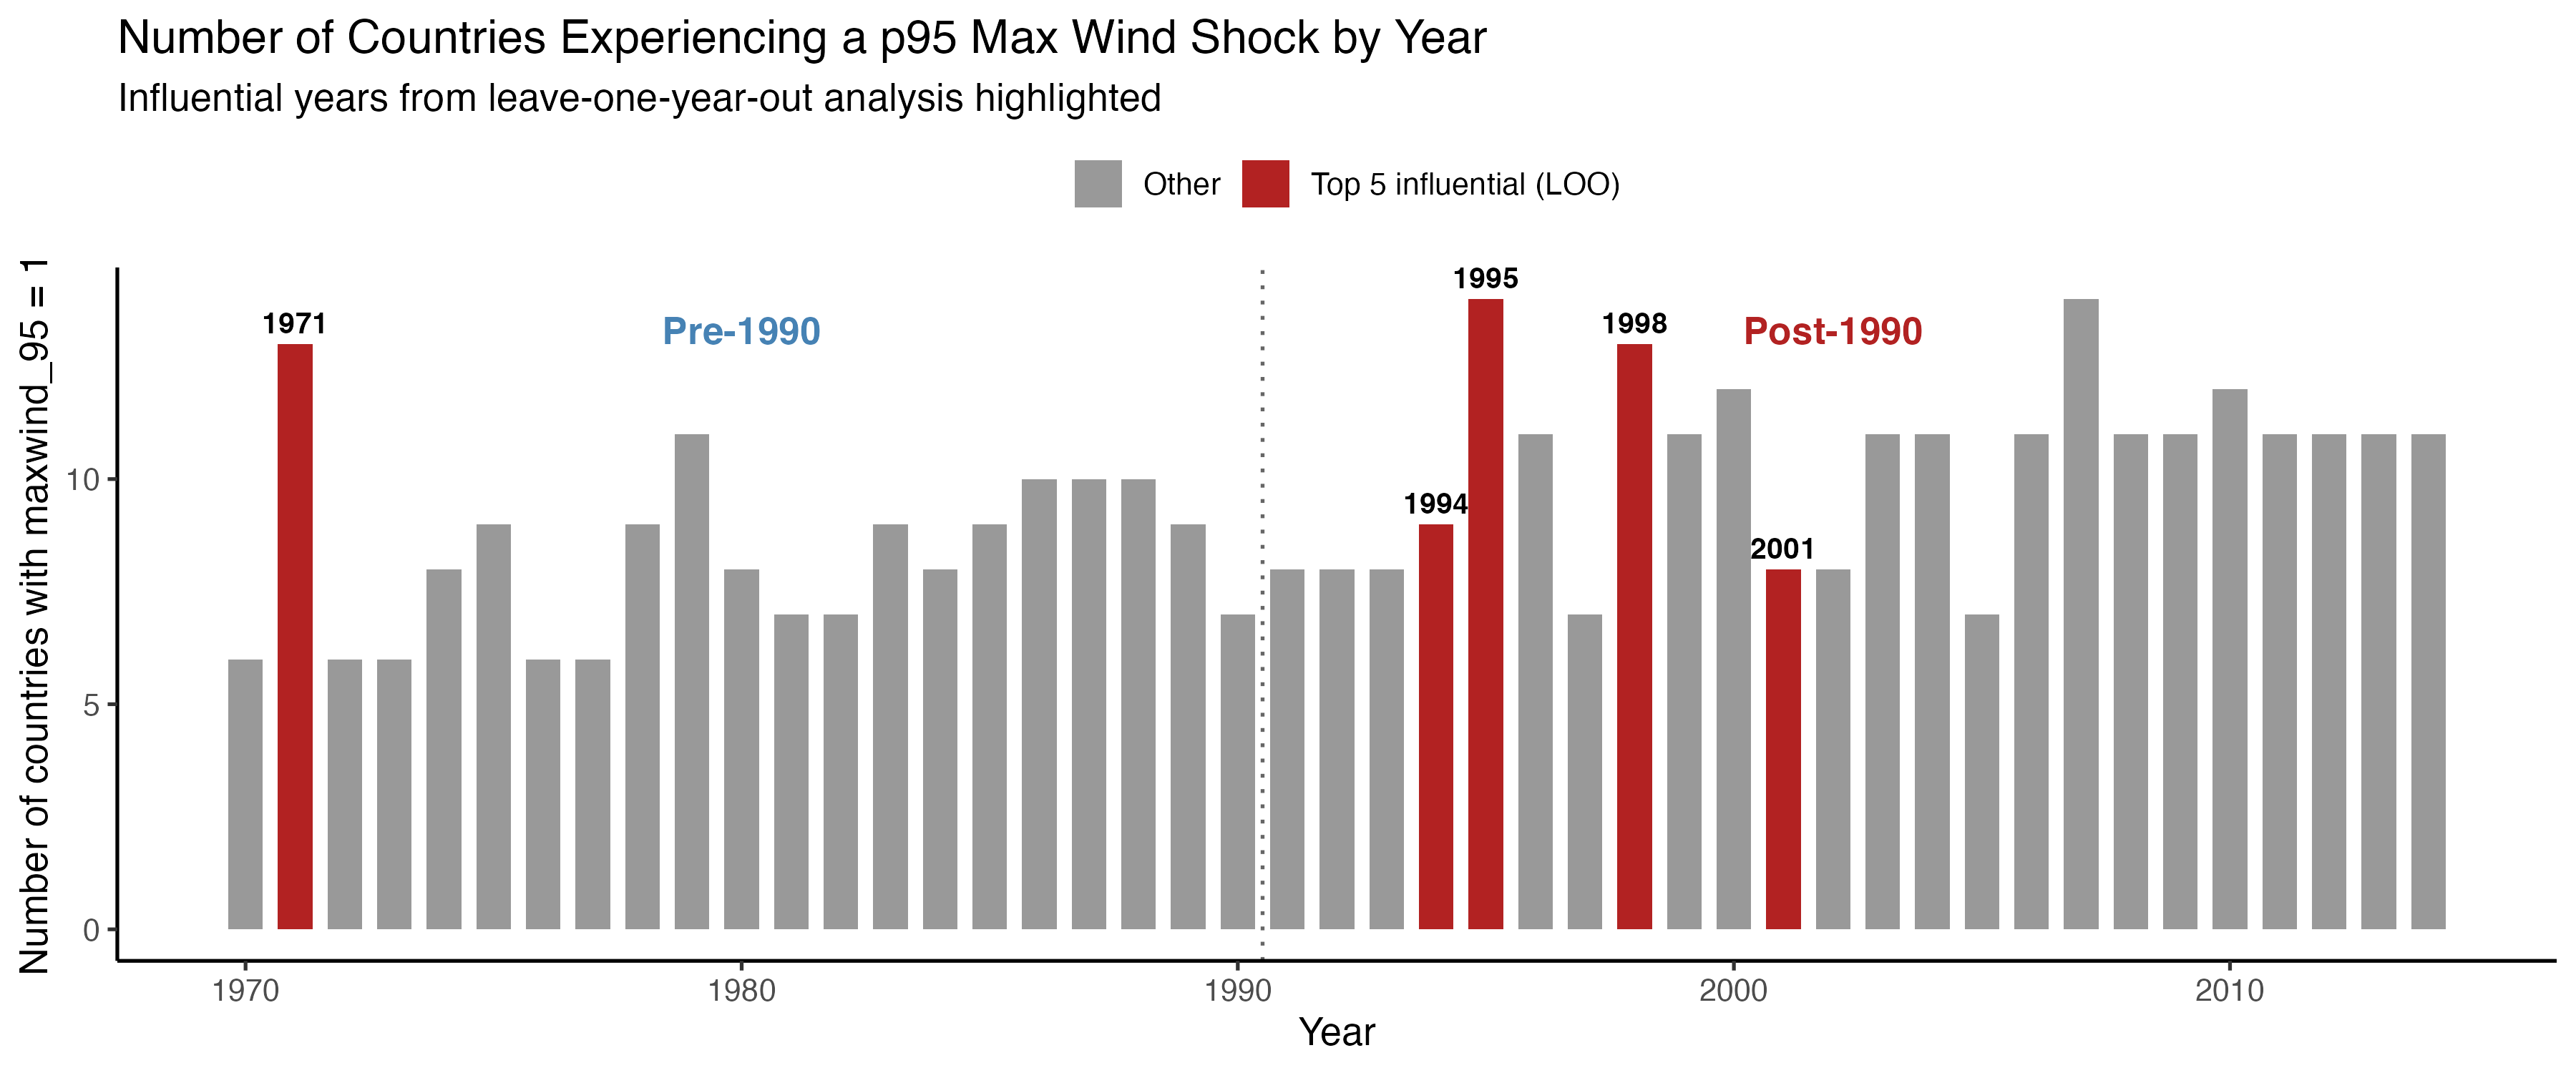
\includegraphics[width=\textwidth,height=0.82\textheight,keepaspectratio]{figures/shock_events_timeline.png}
\end{frame}

% ===============================================================
\section{Estimation}
% ===============================================================

{\hideframenumber
\begin{frame}
\sectionpage
\end{frame}
\showframenumber}

\begin{frame}{Local Projection Specification}
For each horizon $h = 0, 1, \dots, 10$:
\[
  y_{i,t+h} - y_{i,t-1} = \beta_h \, \text{Shock}_{it} + \gamma_h' X_{it} + \alpha_i + \delta_t + \varepsilon_{it}
\]
\begin{itemize}
  \item $y_{it}$: log real GDP per capita
  \item $X_{it}$: two lags of GDP growth and two lags of the shock
  \item Fixed effects: country$\times$year, country$\times$year$^2$, year
  \item Inference: Driscoll--Kraay SE (clustered on year)
\end{itemize}
\end{frame}

\begin{frame}{Period Heterogeneity}
Interact the shock with a period indicator (pre/post-1990):
\[
  y_{i,t+h} - y_{i,t-1} = \sum_{p} \beta_h^{p} \, (\mathbf{1}[\text{Period}=p] \times \text{Shock}_{it}) + \gamma_h' X_{it} + \text{FE} + \varepsilon_{it}
\]
Allows the impulse response to differ across the two sub-periods.
\end{frame}

% ===============================================================
\section{Results}
% ===============================================================

{\hideframenumber
\begin{frame}
\sectionpage
\end{frame}
\showframenumber}

\begin{frame}{Binary Shocks --- Baseline IRFs}
\centering
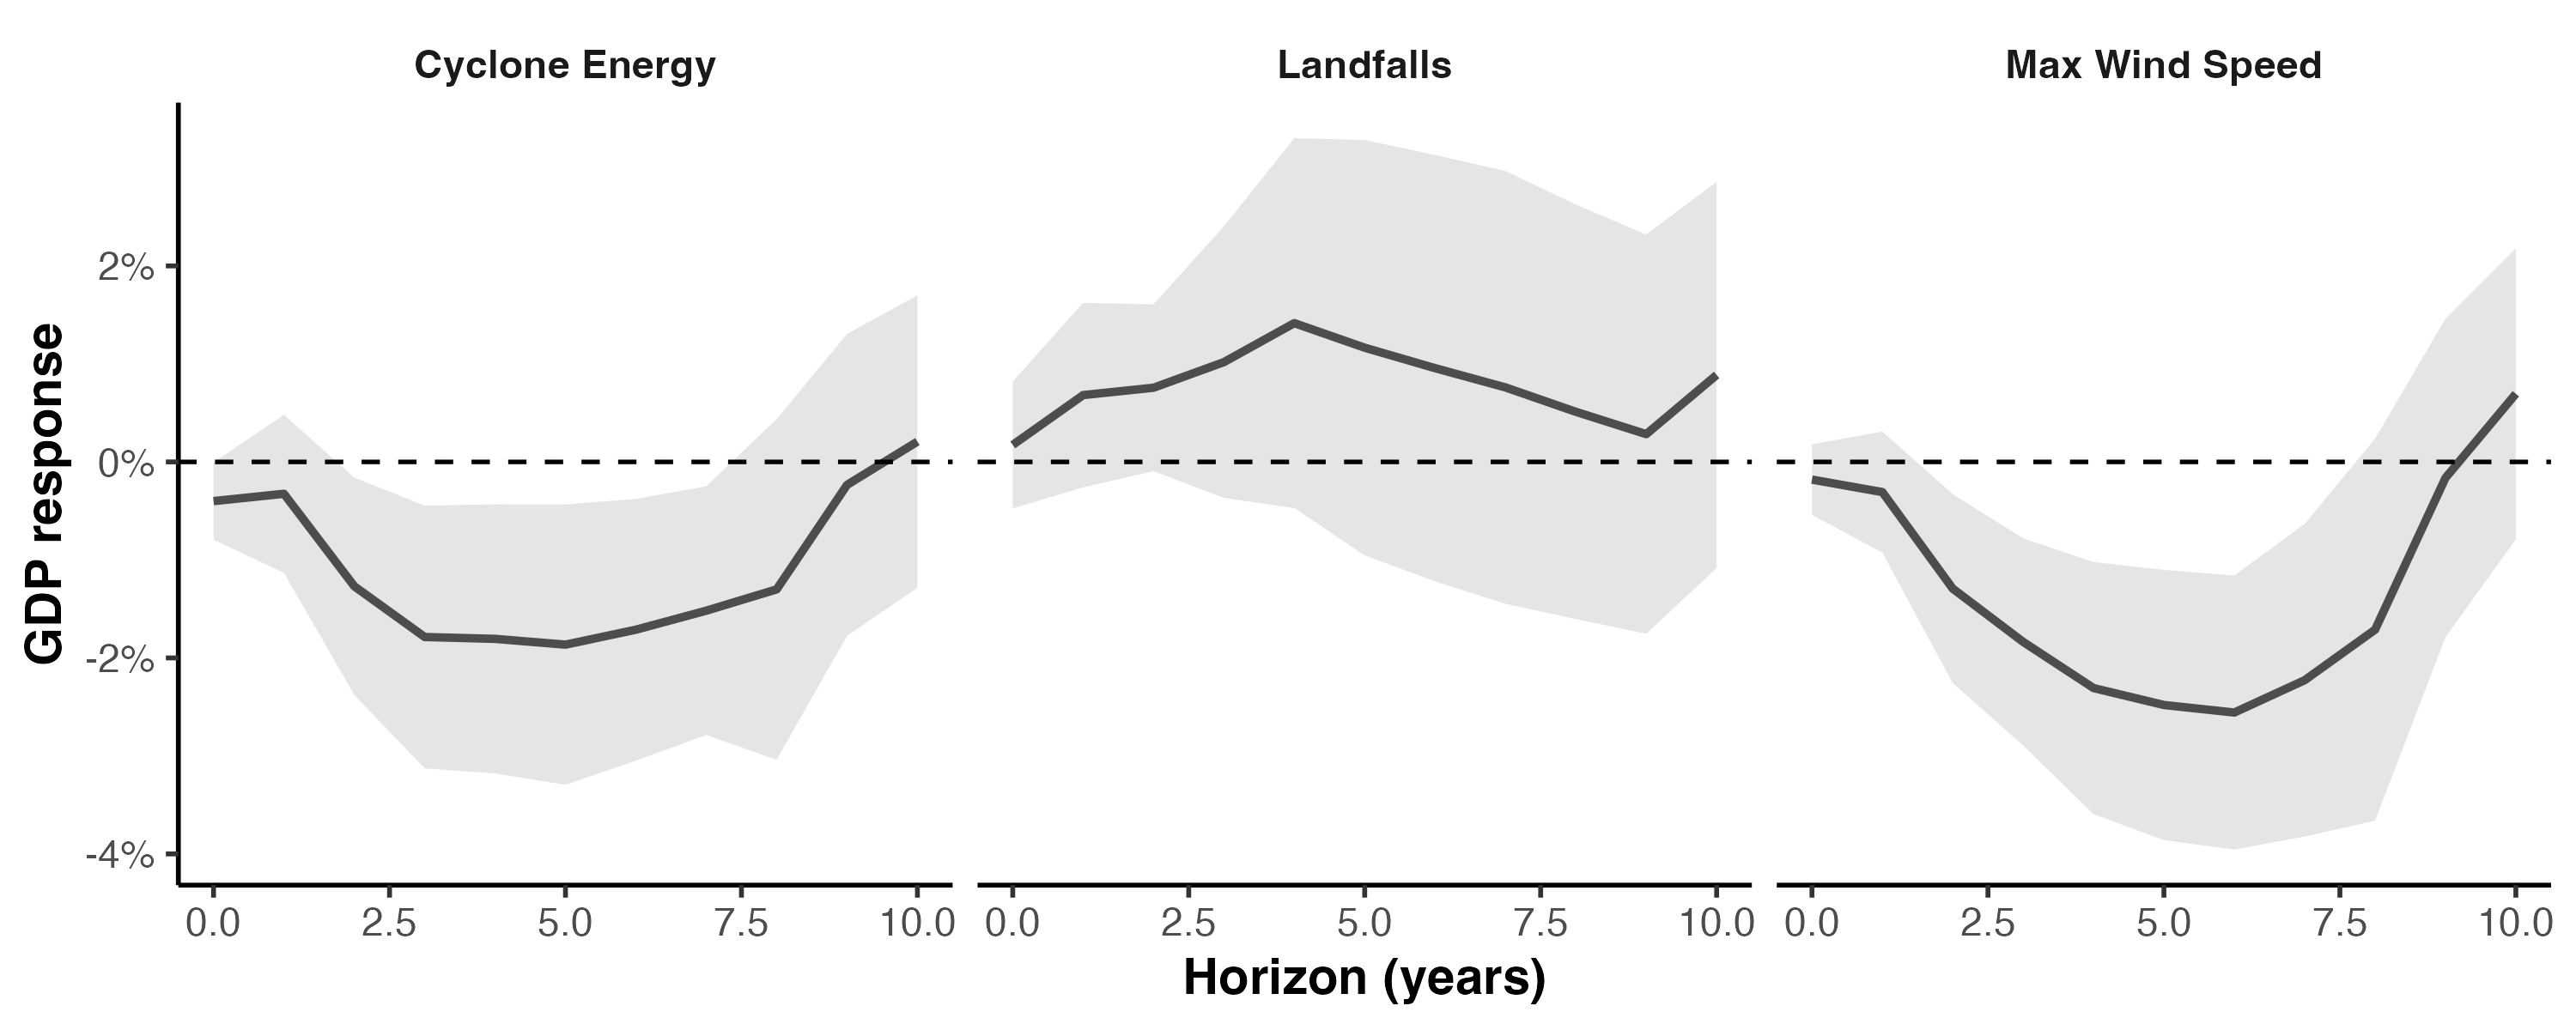
\includegraphics[width=\textwidth]{../figures/irf_all_shocks_95.png}

\smallskip
Negative GDP impact from wind and energy shocks, peaking around $h = 5$.
\end{frame}

\begin{frame}{Binary Shocks --- Pre- vs.\ Post-1990}
\centering
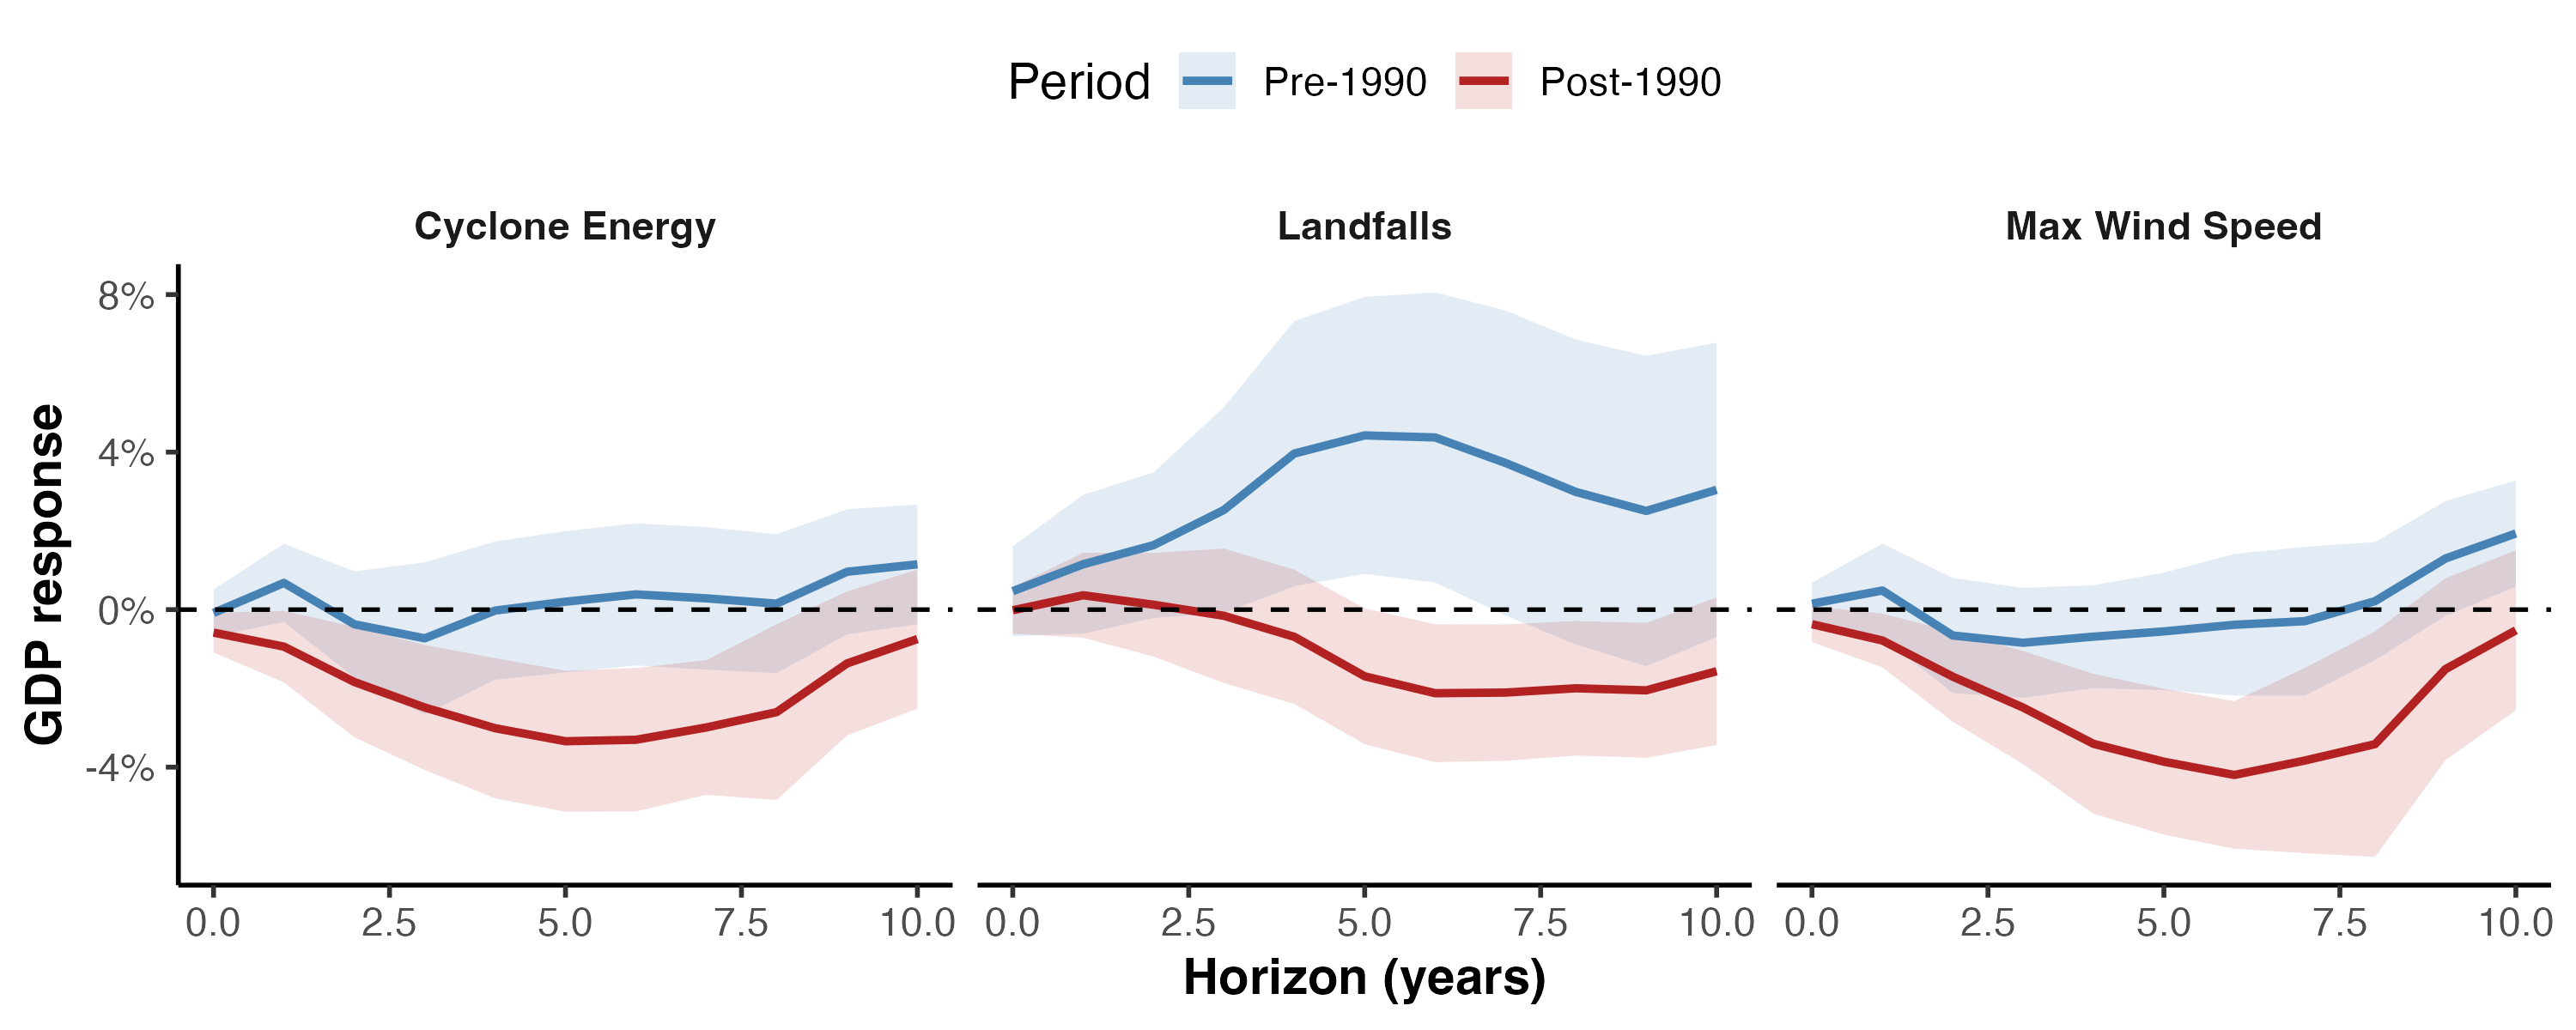
\includegraphics[width=\textwidth]{../figures/irf_all_shocks_95_by_period.png}

\smallskip
Post-1990 shocks appear to produce larger and more persistent GDP losses.
\end{frame}

\begin{frame}{Continuous Shocks --- Baseline IRFs}
\centering
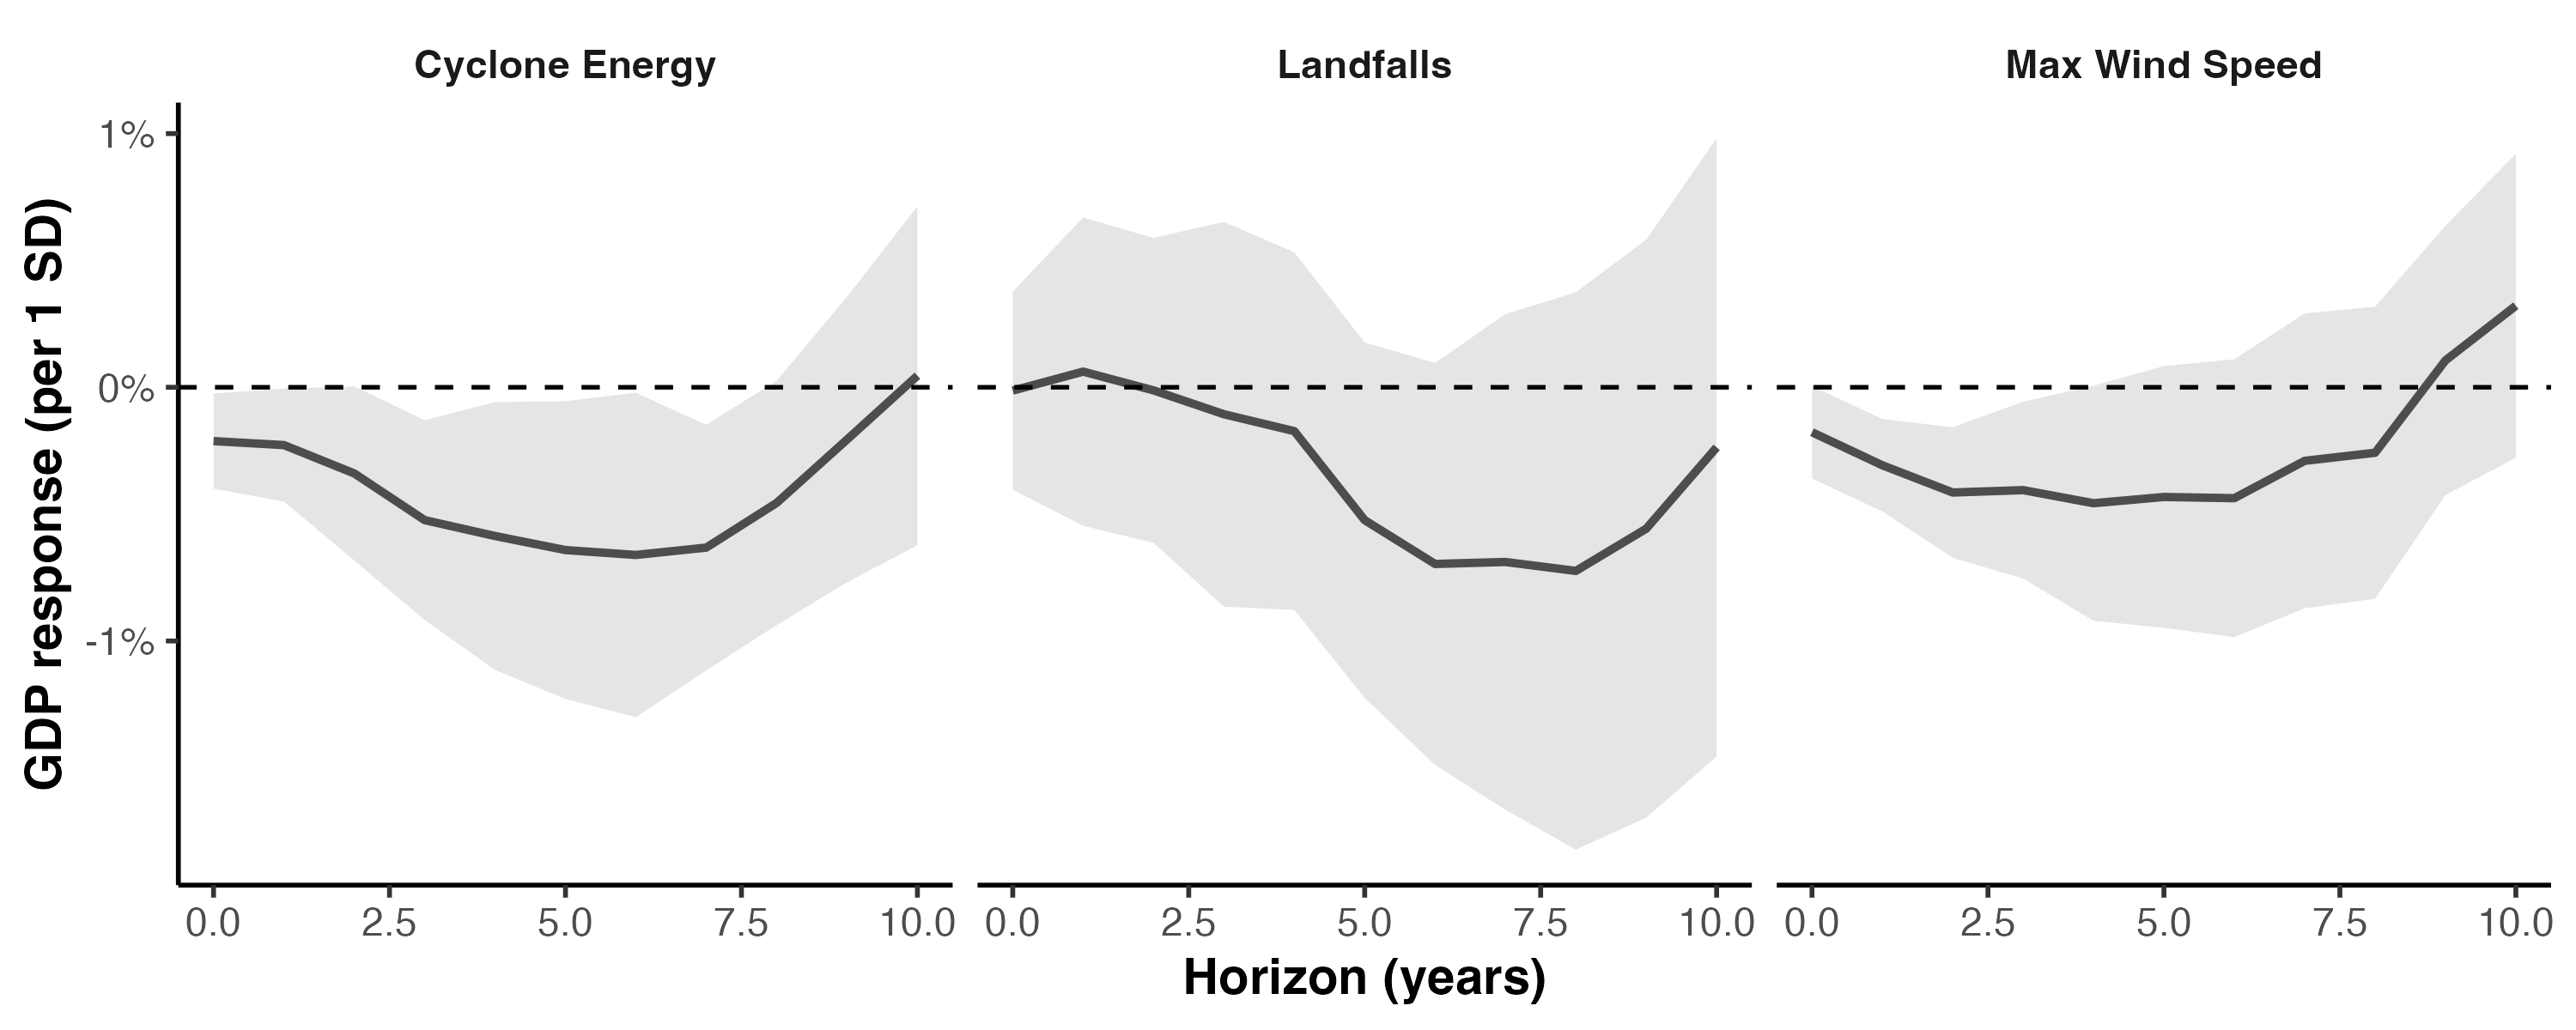
\includegraphics[width=\textwidth]{../figures/irf_all_shocks_continuous.png}

\smallskip
Per 1-SD increase: up to $-0.7\%$ (energy). Similar shape to binary results.
\end{frame}

\begin{frame}{Continuous Shocks --- Pre- vs.\ Post-1990}
\centering
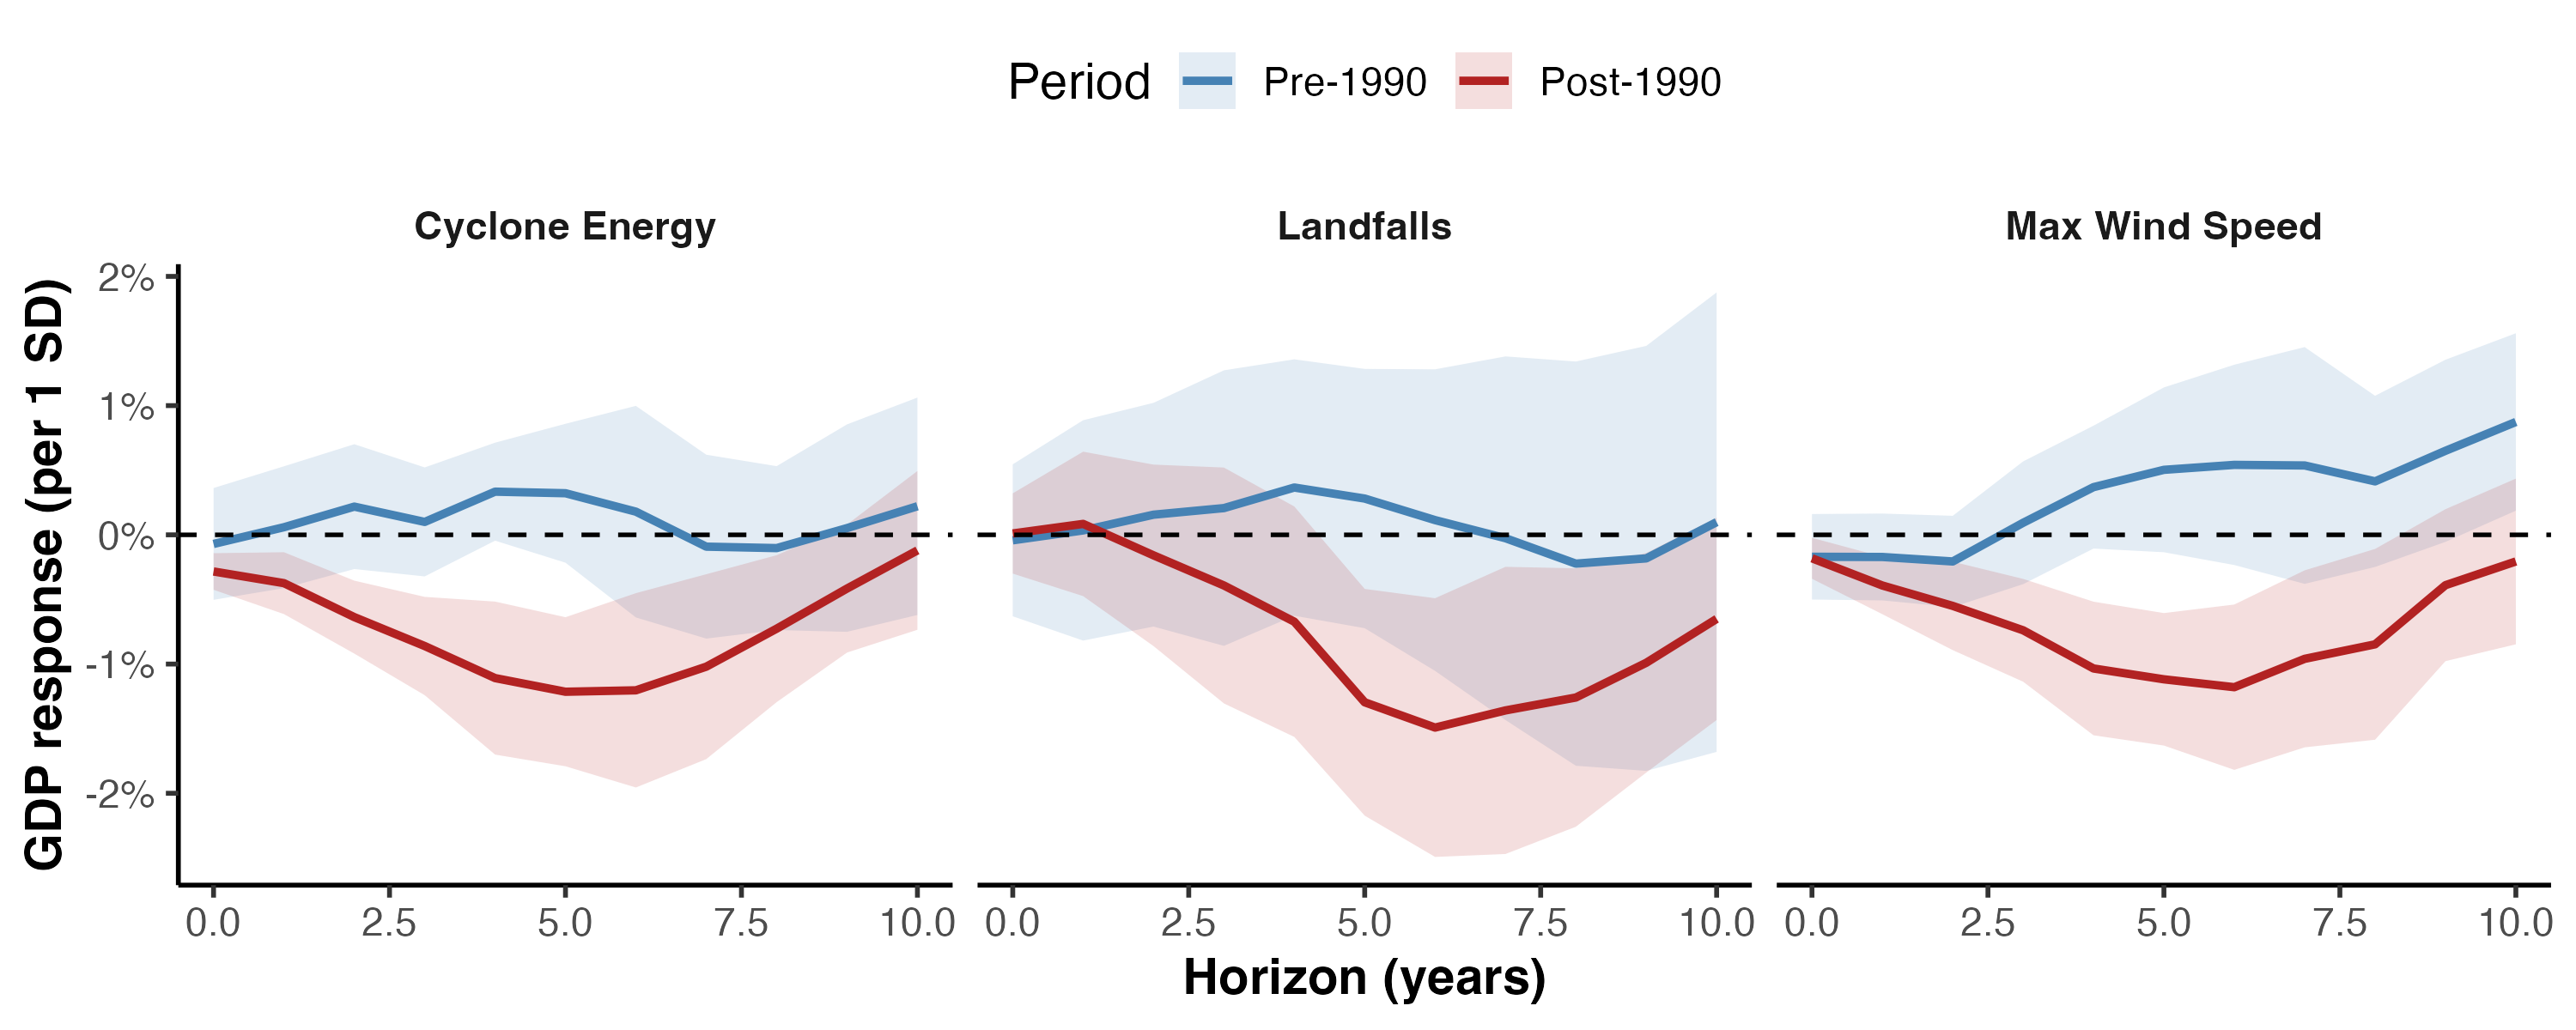
\includegraphics[width=\textwidth]{../figures/irf_all_shocks_continuous_by_period.png}

\smallskip
Period split holds with continuous measures: post-1990 responses are more negative.
\end{frame}

% ===============================================================
\section{Diagnosing the Period Divergence}
% ===============================================================

{\hideframenumber
\begin{frame}
\sectionpage
\end{frame}
\showframenumber}

\begin{frame}{The Puzzle}
Post-1990 cyclone shocks produce much larger GDP losses than pre-1990.
\bigskip

Hypotheses investigated:
\begin{enumerate}
  \item Measurement artifacts (satellite era?)
  \item Shock clustering (serial correlation?)
  \item A discrete 1990 structural break?
  \item Income heterogeneity (who is affected?)
  \item Structural channels (capital, trade, investment?)
  \item \textbf{Control group composition} ($\to$ key finding)
\end{enumerate}
\end{frame}

% - - - - - - - - - - - - - - - - - - - - - - - - - - - - - - -
\subsection{Measurement Artifacts}
% - - - - - - - - - - - - - - - - - - - - - - - - - - - - - - -

{\hideframenumber
\begin{frame}
\subsectionpage
\end{frame}
\showframenumber}

\begin{frame}{Cyclone Exposure Time Series}
\centering
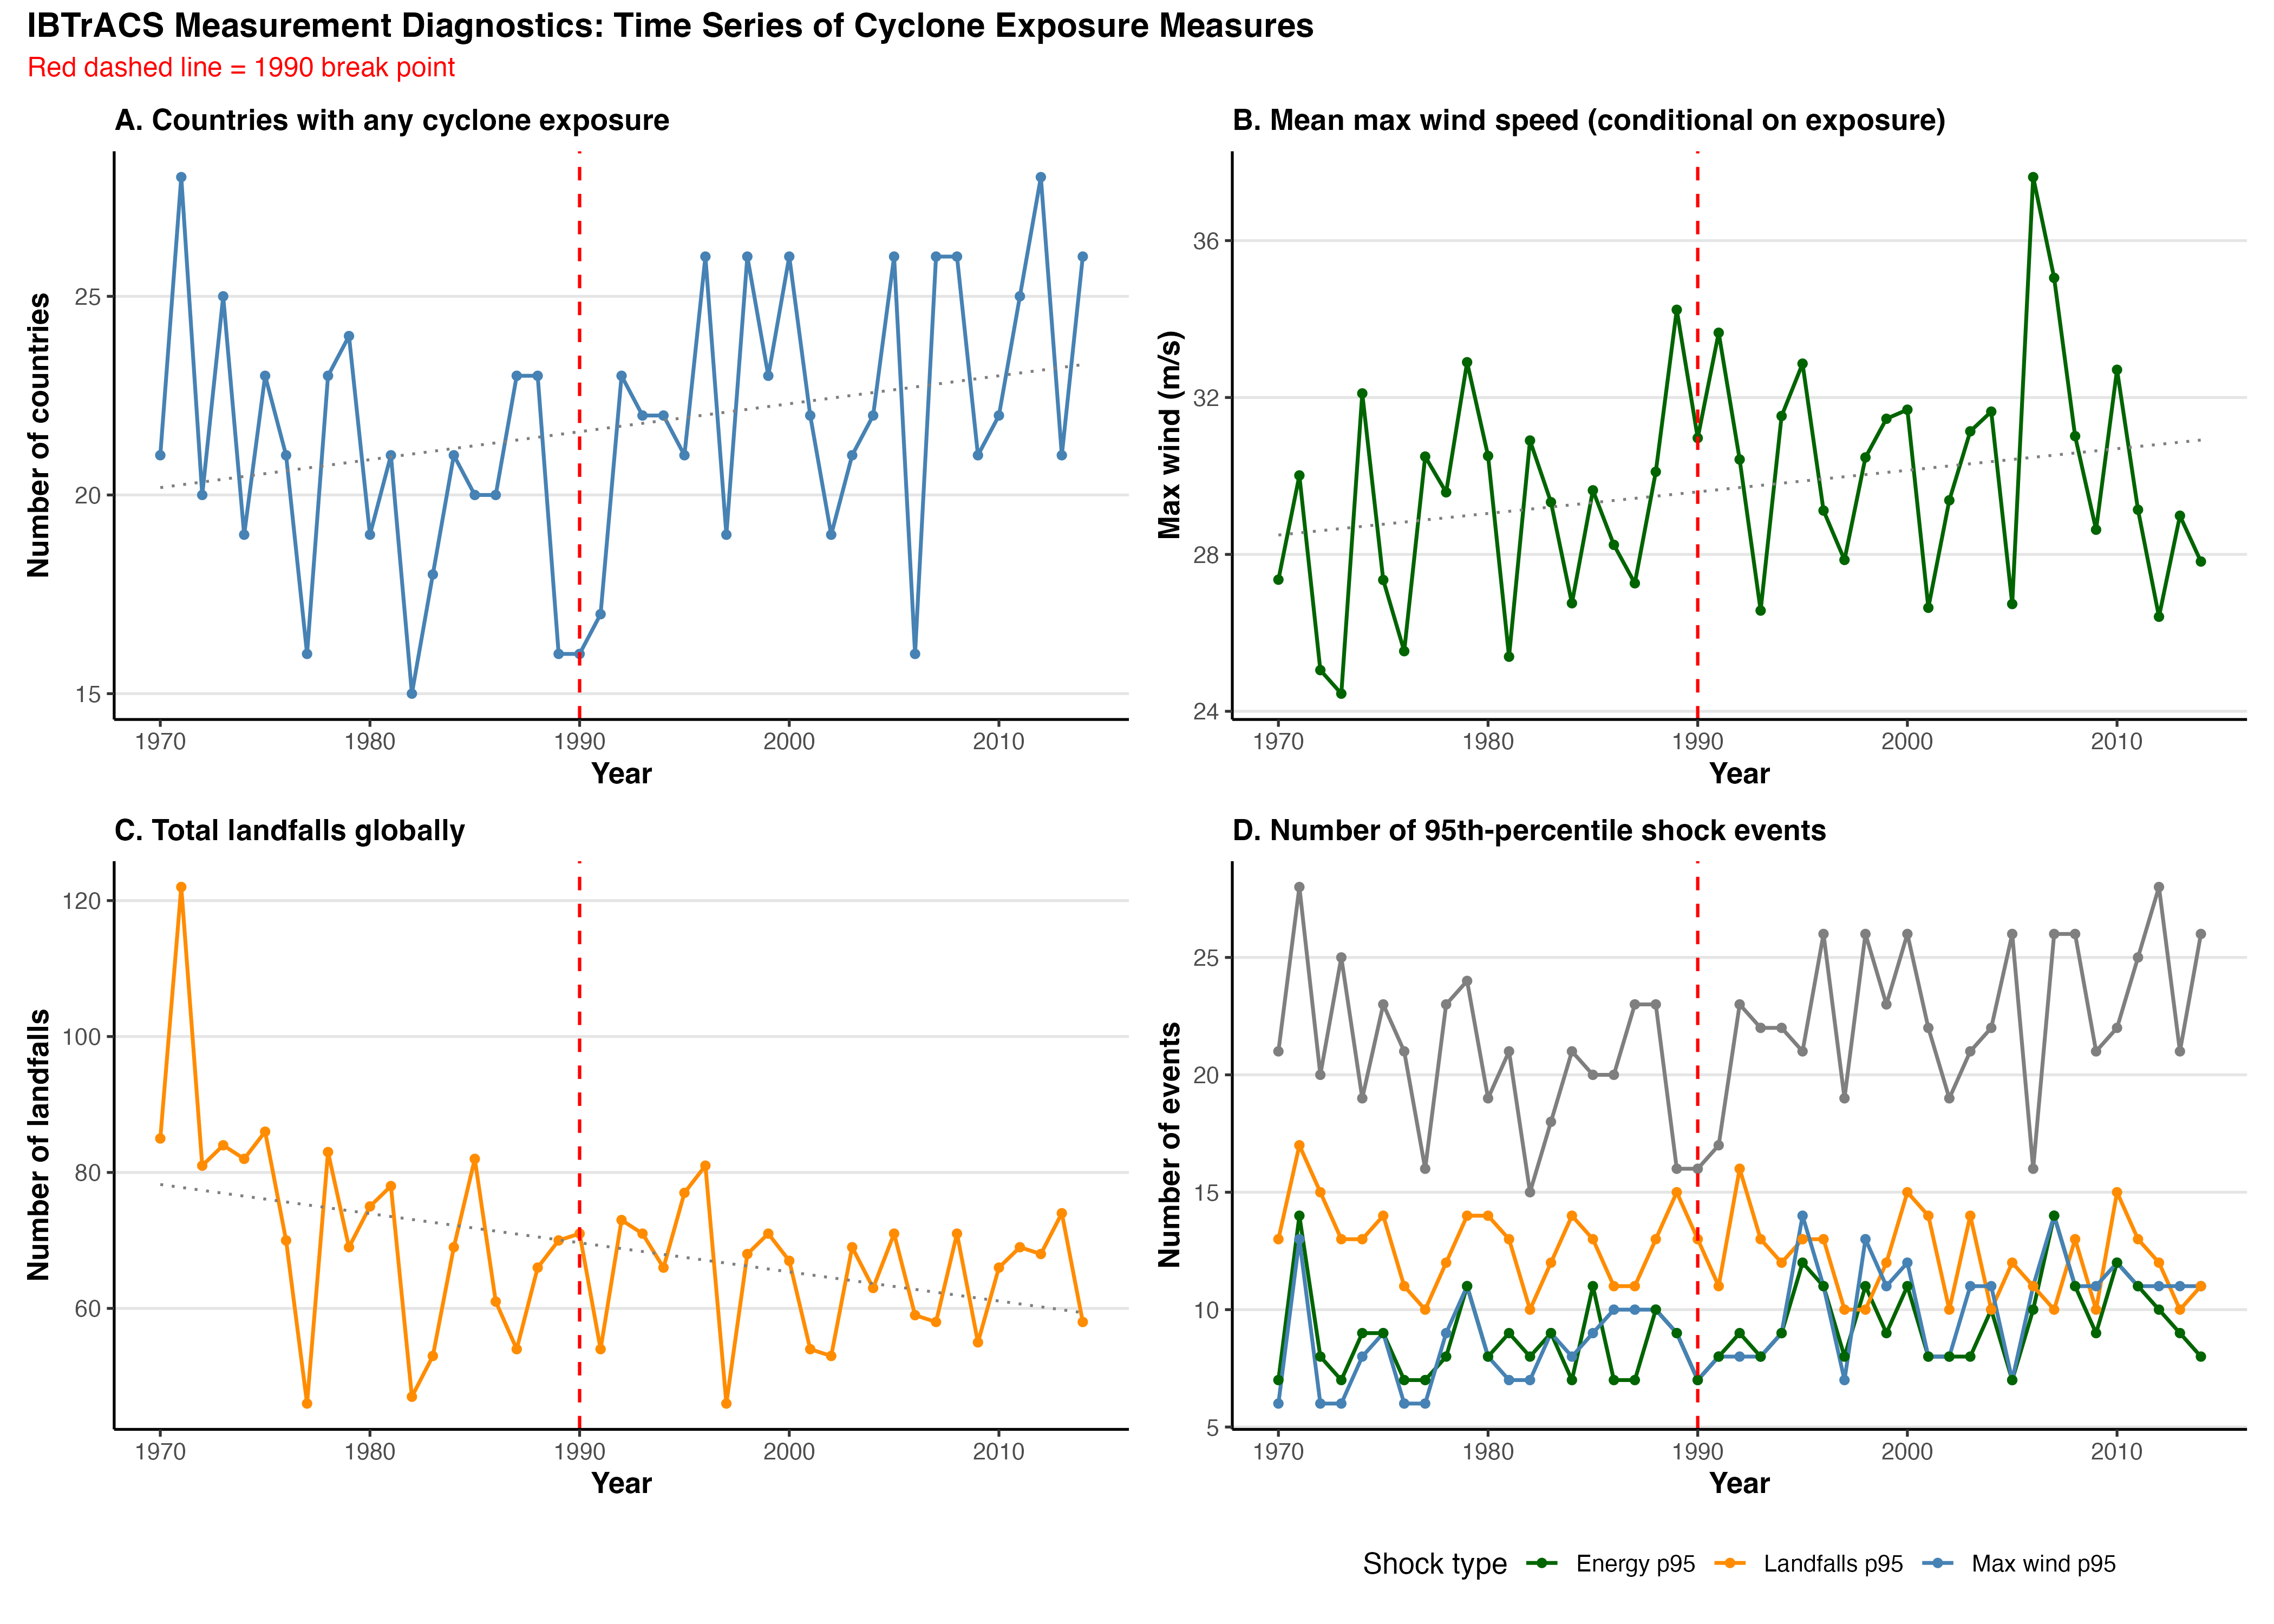
\includegraphics[width=\textwidth,height=0.82\textheight,keepaspectratio]{figures/measurement_timeseries.png}
\end{frame}

\begin{frame}{Wind Speed Distributions by Period}
\centering
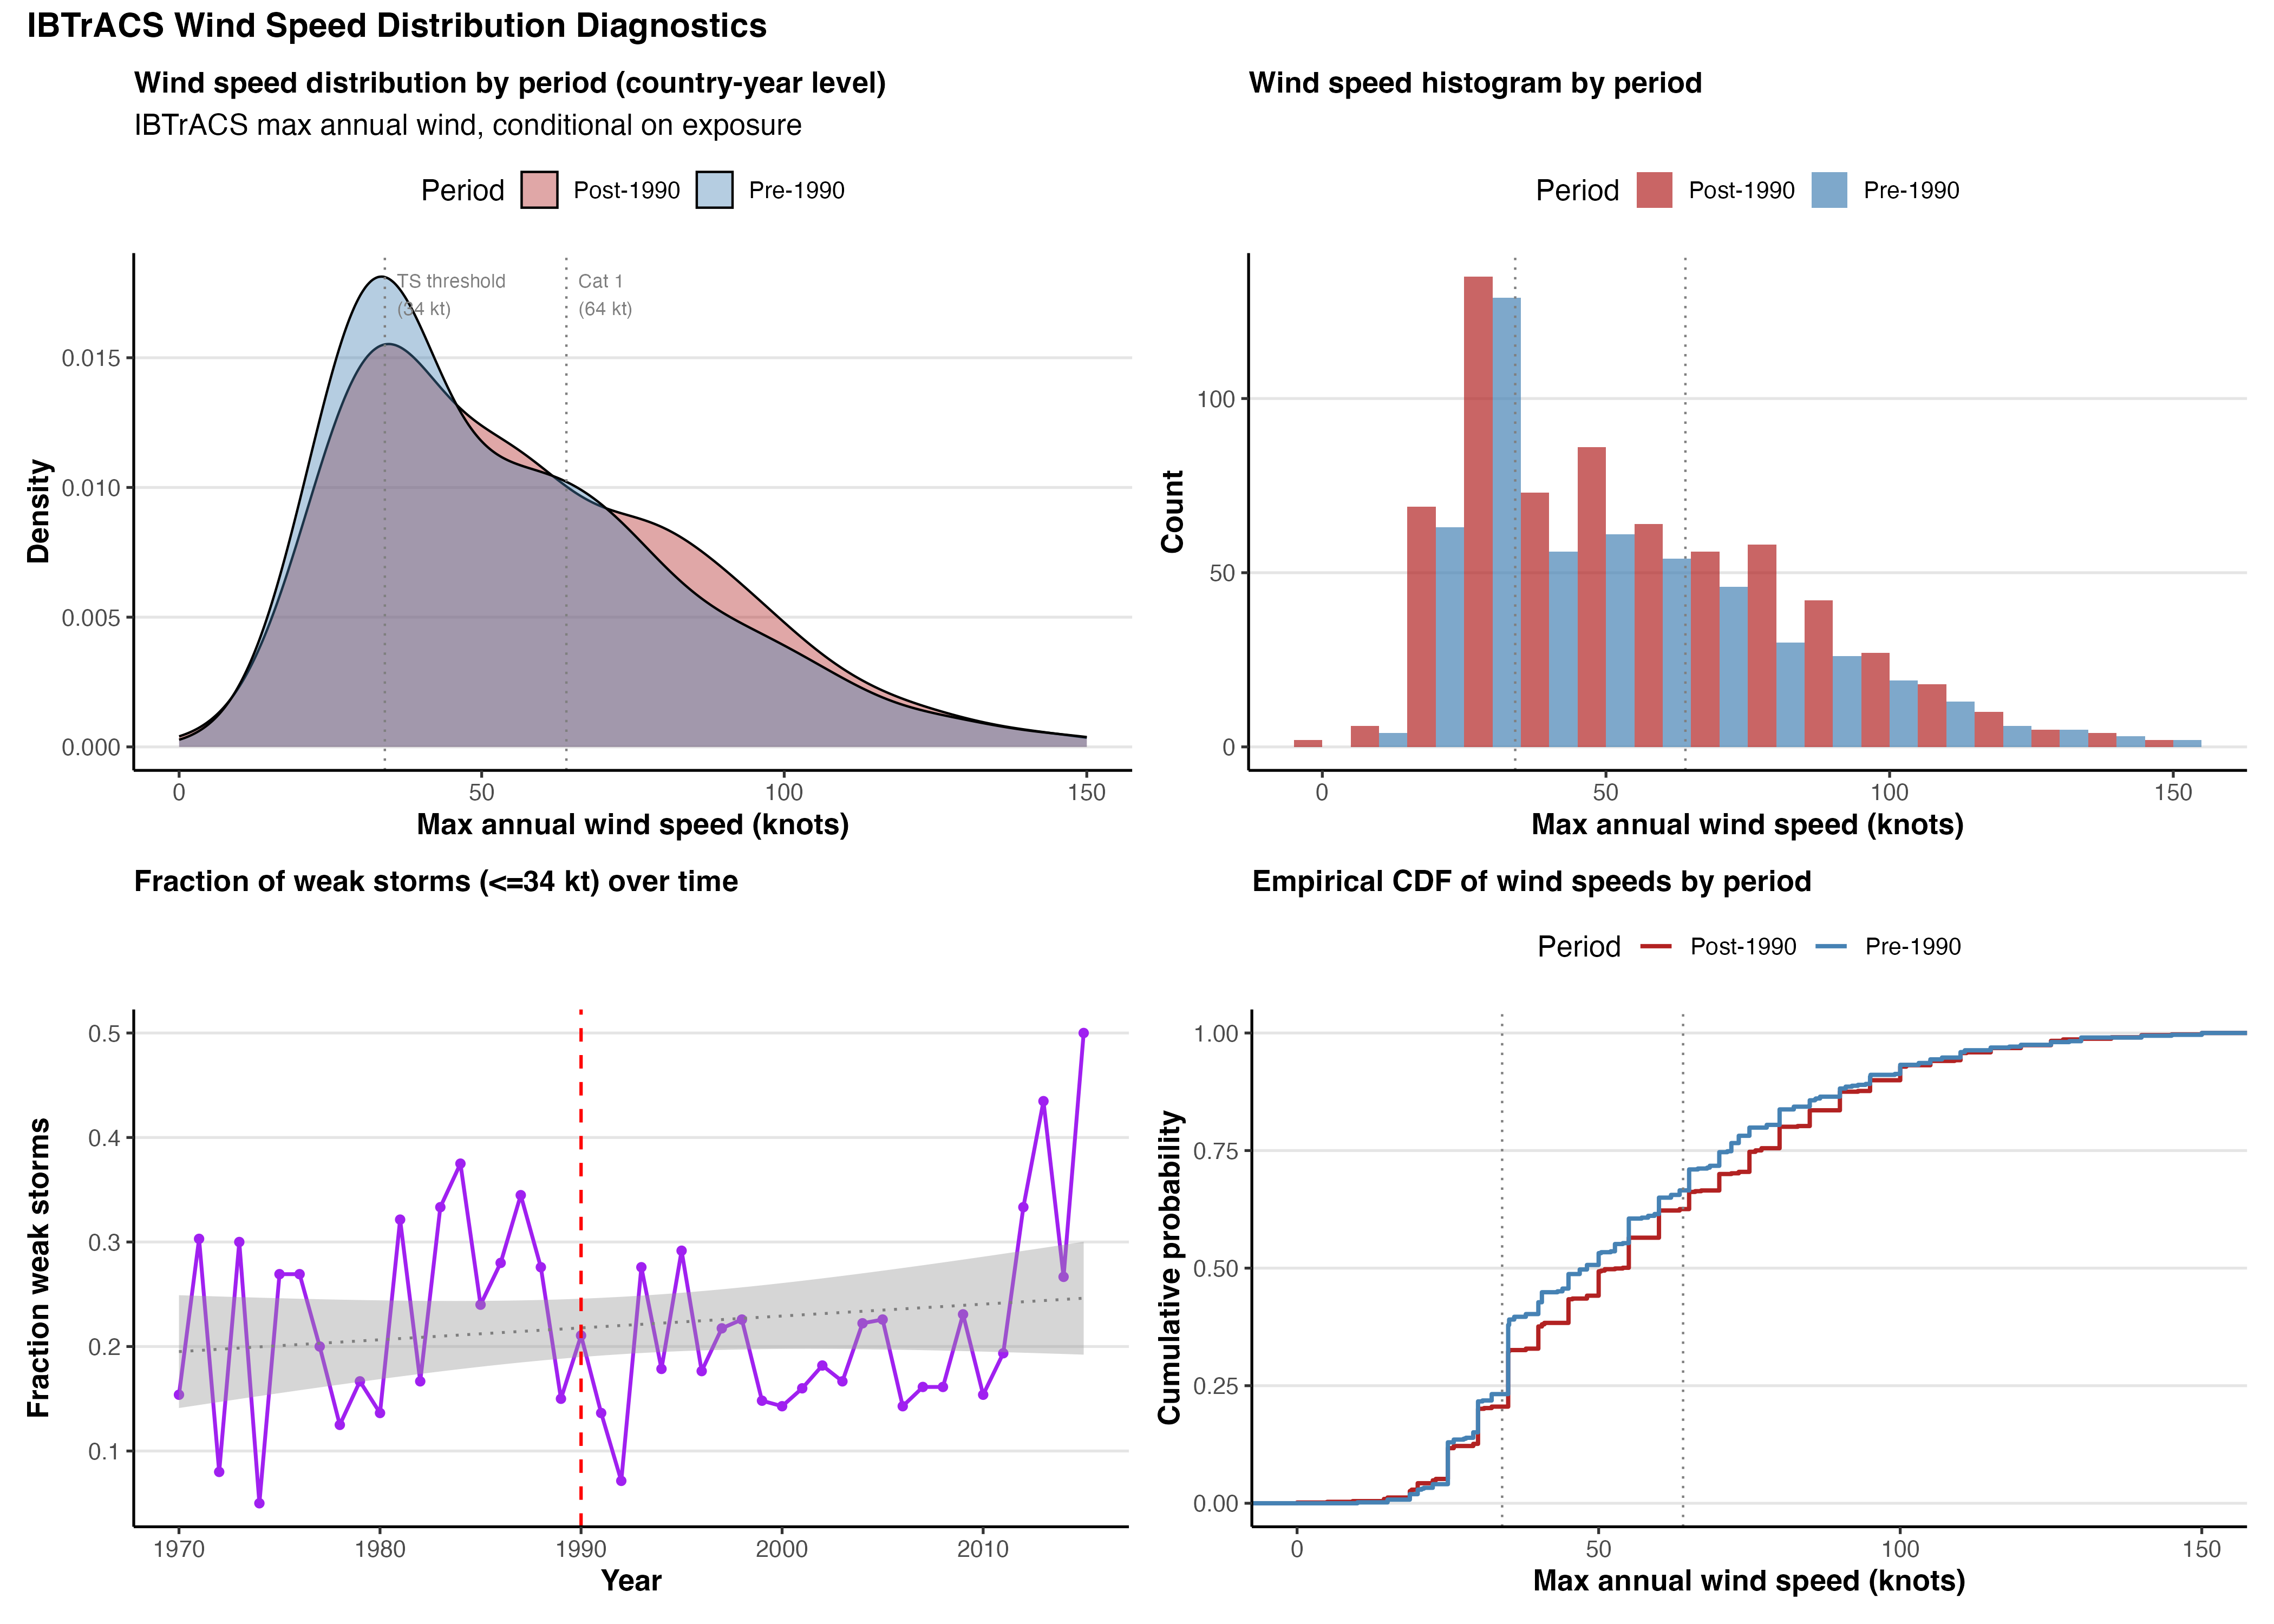
\includegraphics[width=\textwidth,height=0.82\textheight,keepaspectratio]{figures/measurement_wind_distribution.png}
\end{frame}

\begin{frame}{Ruled Out: Measurement Artifacts}
\begin{itemize}
  \item No jump in recorded cyclone counts around 1990 ($p = 0.30$)
  \item Wind speeds are \emph{higher} post-1990 (57.5 vs.\ 54.6 knots) --- opposite of detection bias
  \item Fraction of weak storms unchanged (22.6\% vs.\ 21.6\%, $p = 0.71$)
  \item Landfalls actually \emph{decline} post-1990
  \item Chow test for structural break at 1990: $p = 0.94$
\end{itemize}
\bigskip
Improved satellite tracking does not explain the divergence.
\end{frame}

% - - - - - - - - - - - - - - - - - - - - - - - - - - - - - - -
\subsection{Shock Clustering}
% - - - - - - - - - - - - - - - - - - - - - - - - - - - - - - -

{\hideframenumber
\begin{frame}
\subsectionpage
\end{frame}
\showframenumber}

\begin{frame}{Ruled Out: Shock Clustering}
\begin{itemize}
  \item Consecutive-exposure rate nearly identical: 65.7\% pre vs.\ 67.8\% post
  \item Within-country AR(1) of wind speed $\approx 0$ in both periods
  \item Mean inter-shock gap actually \emph{longer} post-1990 (2.3 vs.\ 1.7 years)
\end{itemize}
\bigskip
The ``no time to recover'' hypothesis is not supported.
\end{frame}

% - - - - - - - - - - - - - - - - - - - - - - - - - - - - - - -
\subsection{Breakpoint Location}
% - - - - - - - - - - - - - - - - - - - - - - - - - - - - - - -

{\hideframenumber
\begin{frame}
\subsectionpage
\end{frame}
\showframenumber}

\begin{frame}{Breakpoint Robustness}
\centering
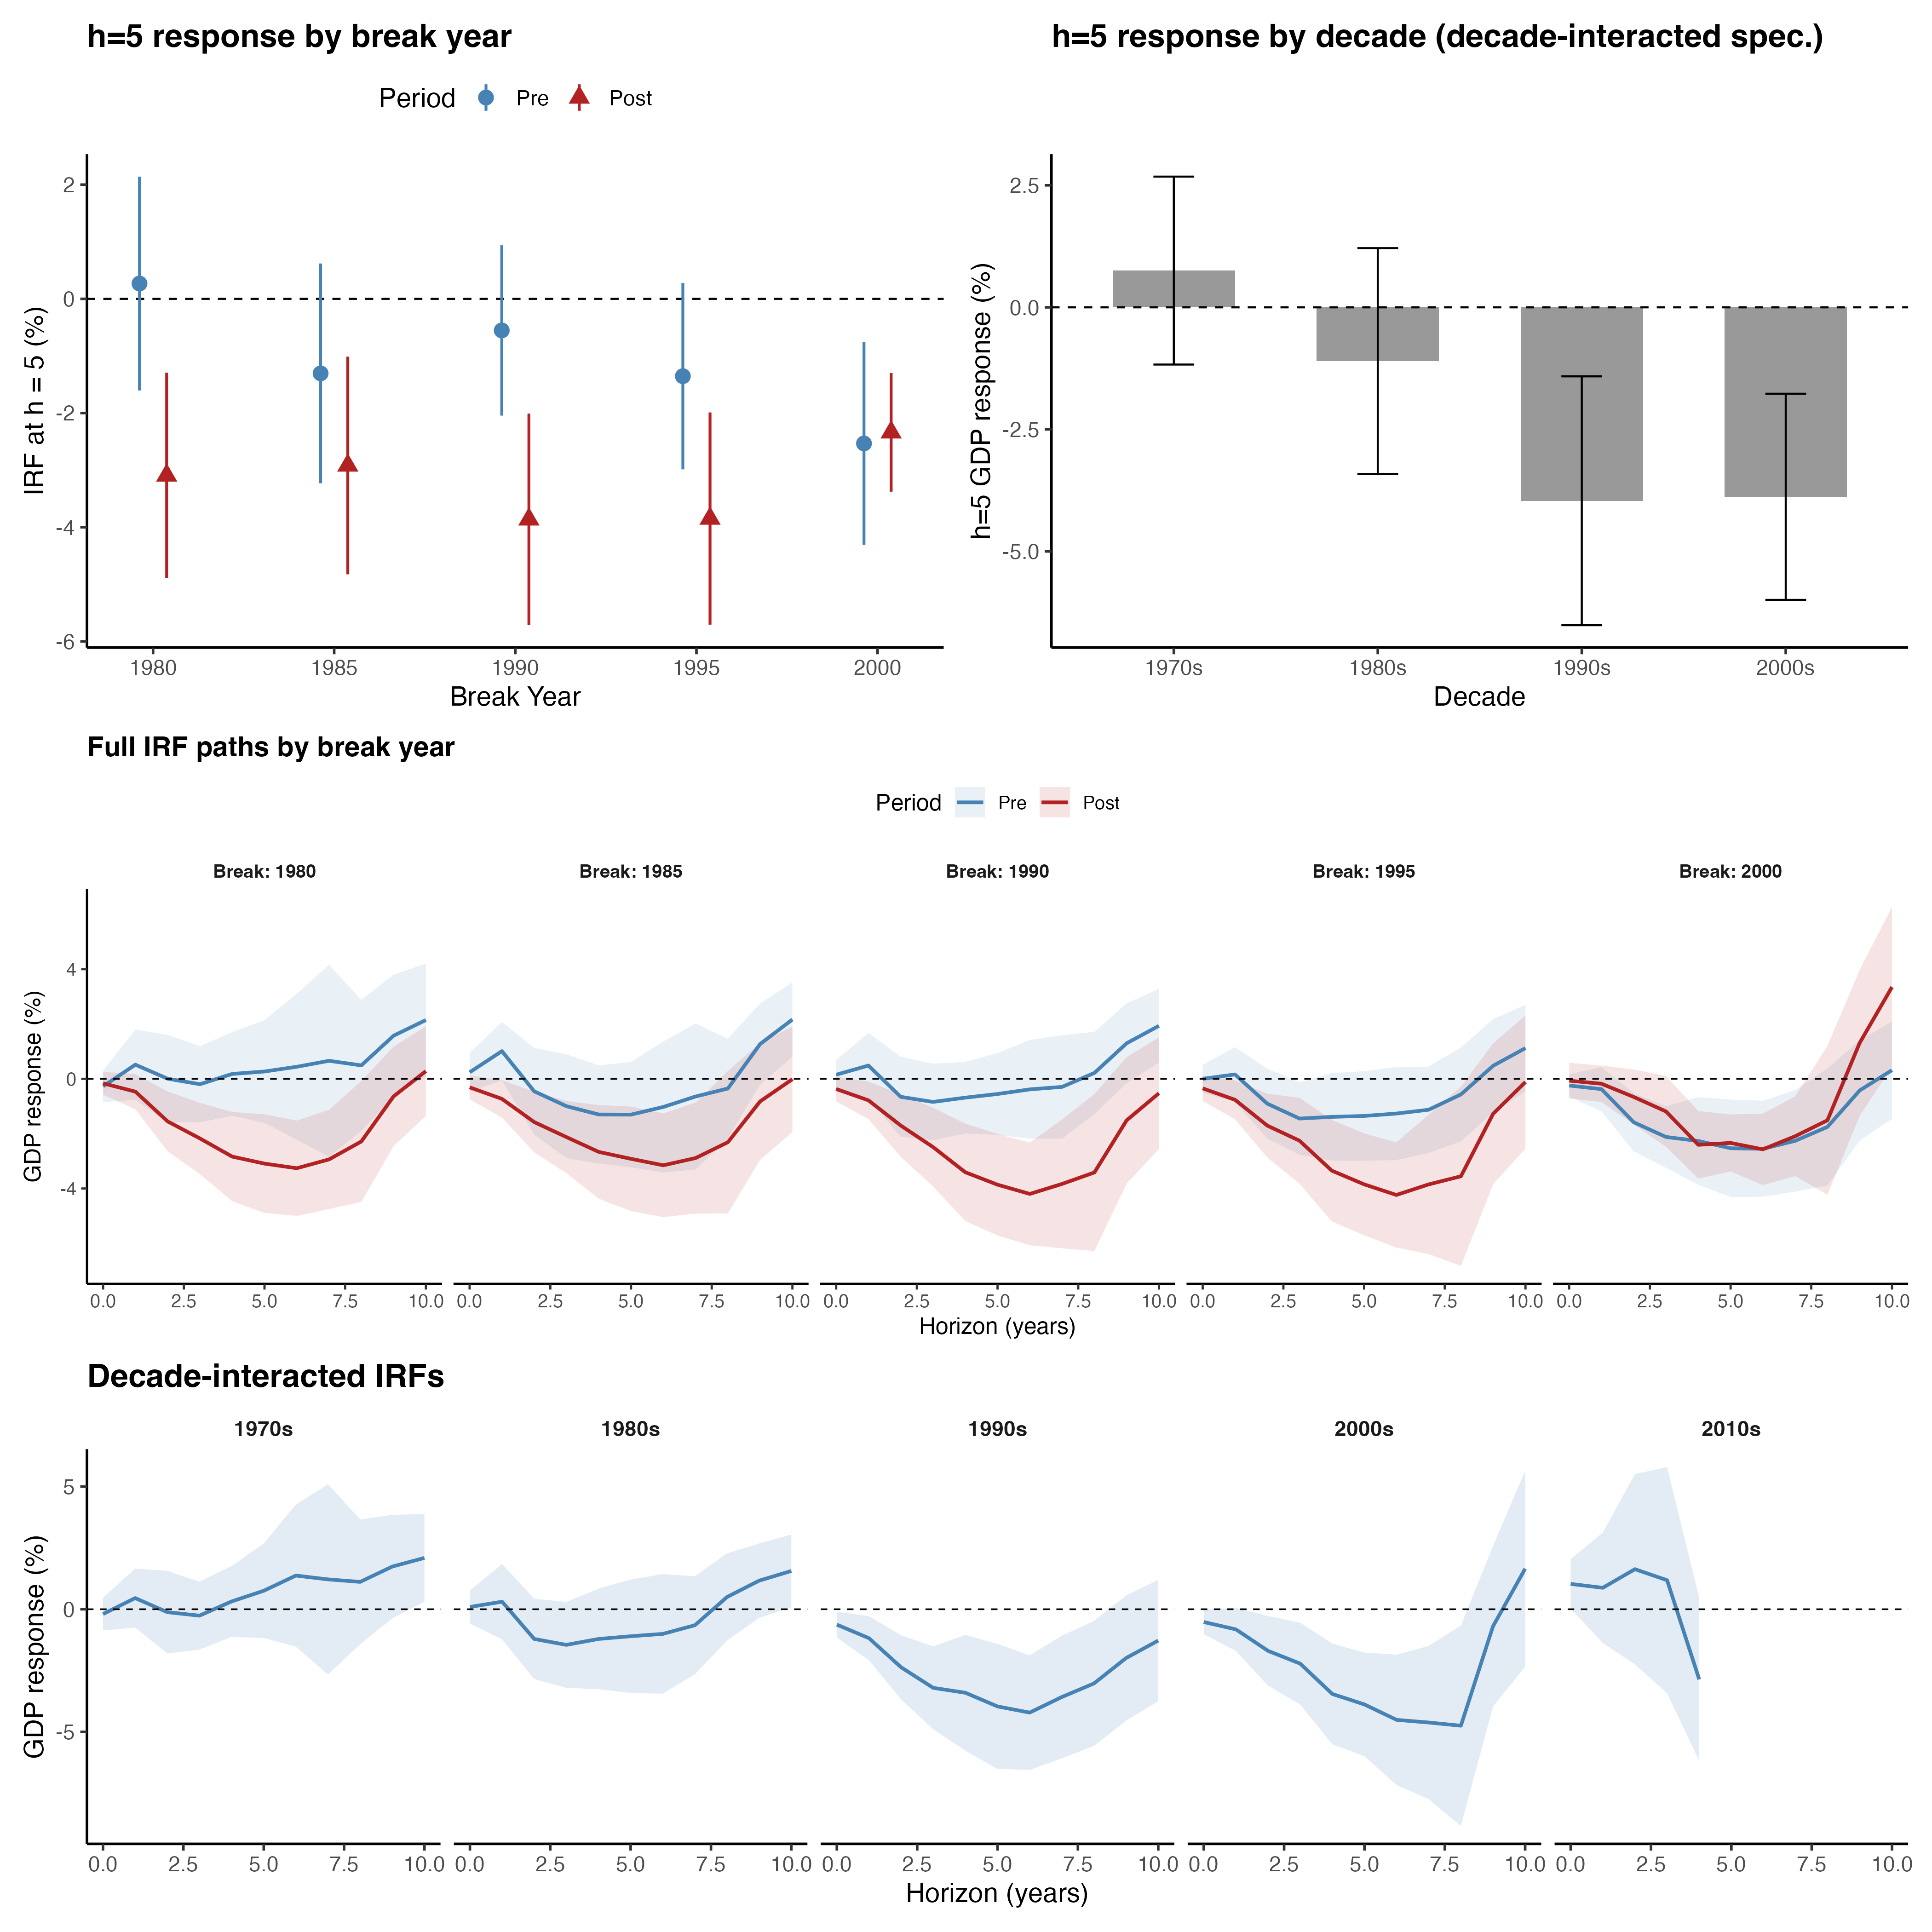
\includegraphics[width=\textwidth,height=0.85\textheight,keepaspectratio]{figures/breakpoint_robustness.png}
\end{frame}

\begin{frame}{Not a Discrete Break --- A Gradual Shift}
Decade-by-decade IRFs at $h = 5$ (maxwind p95 shock):
\medskip

\begin{tabular}{@{}lrl@{}}
  \toprule
  \textbf{1970s} & $+0.75\%$ & insignificant \\
  \textbf{1980s} & $-1.10\%$ & insignificant (transition decade) \\
  \textbf{1990s} & $-3.96\%$ & significant \\
  \textbf{2000s} & $-3.88\%$ & significant \\
  \bottomrule
\end{tabular}
\medskip

The effect builds monotonically from the 1970s and plateaus by the 1990s.
\end{frame}

% - - - - - - - - - - - - - - - - - - - - - - - - - - - - - - -
\subsection{Income Heterogeneity}
% - - - - - - - - - - - - - - - - - - - - - - - - - - - - - - -

{\hideframenumber
\begin{frame}
\subsectionpage
\end{frame}
\showframenumber}

\begin{frame}{IRF by Income Quartile and Period}
\centering

\includegraphics[width=\textwidth,height=0.72\textheight,keepaspectratio]{figures/irf_income_quartiles_by_period.png}

\smallskip
The divergence is concentrated in Q3--Q4 (upper-middle and high income).
\end{frame}

\begin{frame}{Finer Bins: Income Quintiles}
\centering
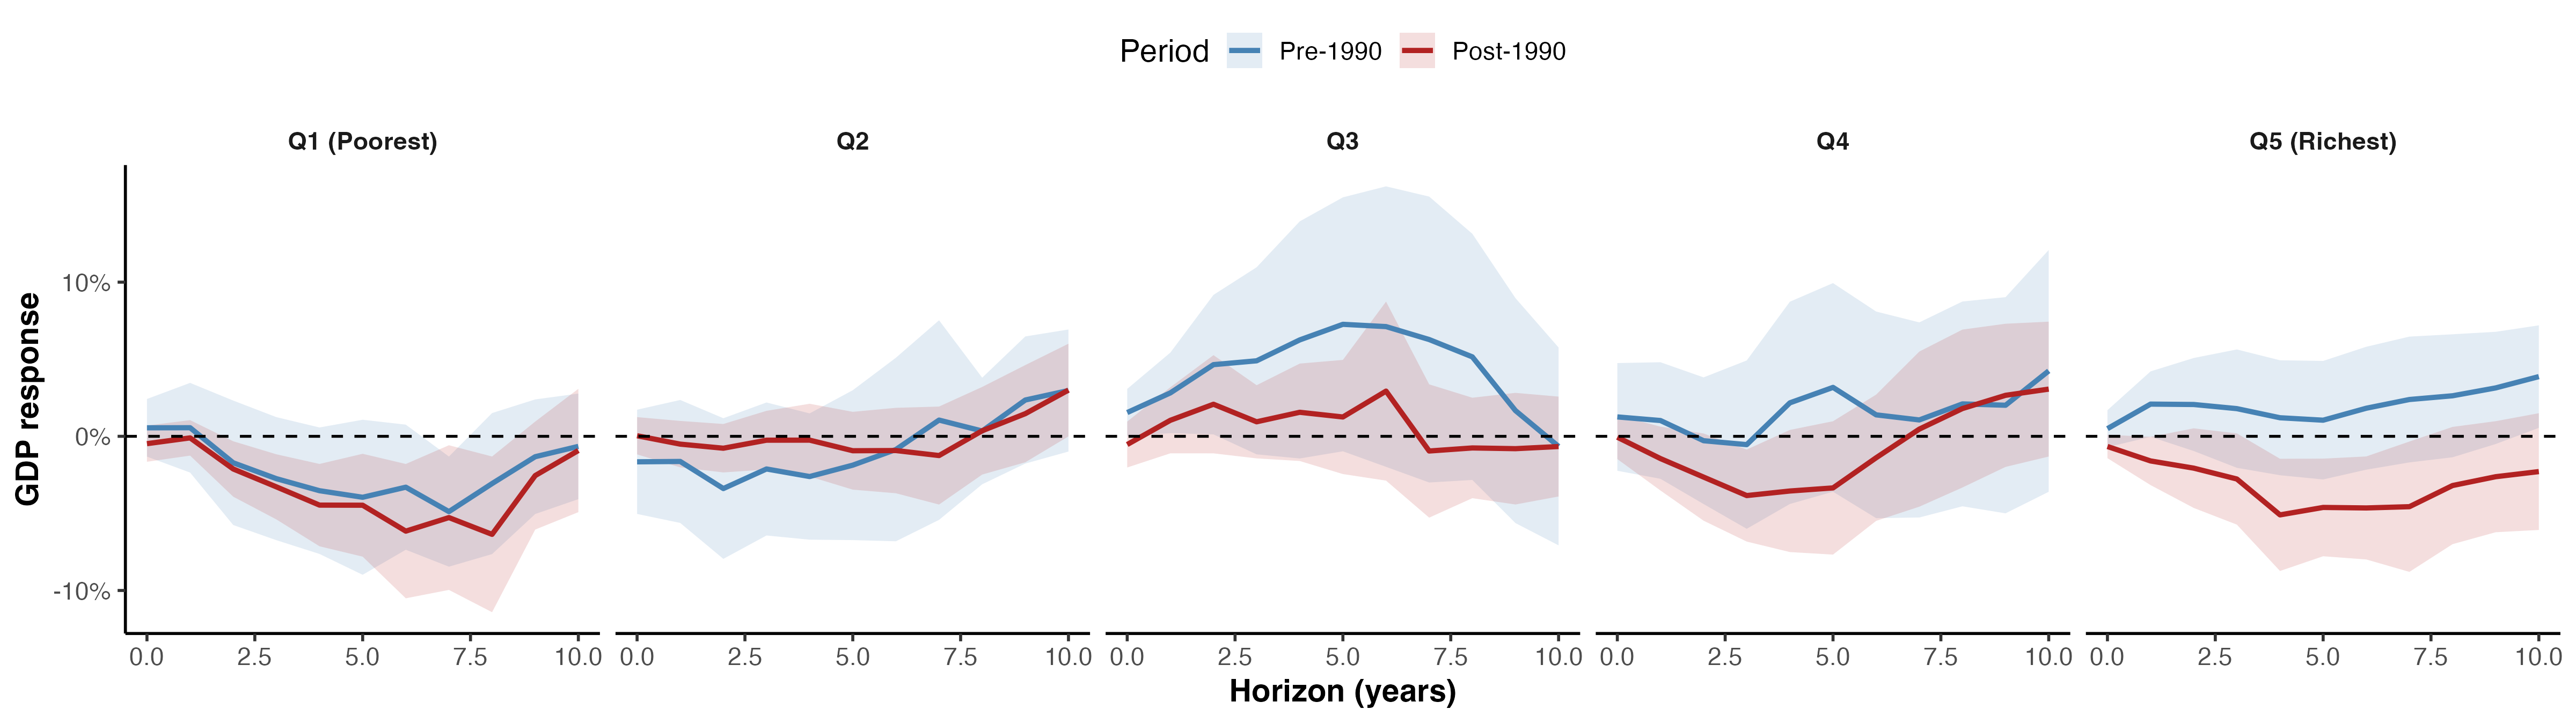
\includegraphics[width=\textwidth,height=0.72\textheight,keepaspectratio]{figures/irf_income_quintiles_by_period.png}

\smallskip
Q3 shows the largest pre-1990 positive response ($+7.3\%$ at $h=5$). Q4--Q5 also flip sign.
\end{frame}

\begin{frame}{Pre-1990: Reconstruction Booms in Rich Countries}
At $h = 5$ (maxwind p95 shock), the pre-1990 IRF by income quintile:
\medskip

\begin{tabular}{@{}lrl@{}}
  \toprule
  \textbf{Q1 (Poorest)} & $-4.0\%$ & negative in both periods \\
  \textbf{Q2} & $-1.9\%$ & small, insignificant \\
  \textbf{Q3} & $+7.3\%$ & reconstruction stimulus \\
  \textbf{Q4} & $+3.2\%$ & reconstruction stimulus \\
  \textbf{Q5 (Richest)} & $+1.0\%$ & positive but imprecise \\
  \bottomrule
\end{tabular}
\medskip

Rich countries experienced \emph{GDP gains} from cyclones pre-1990. This reverses post-1990.
\end{frame}

\begin{frame}{Who Is Exposed?}
\centering
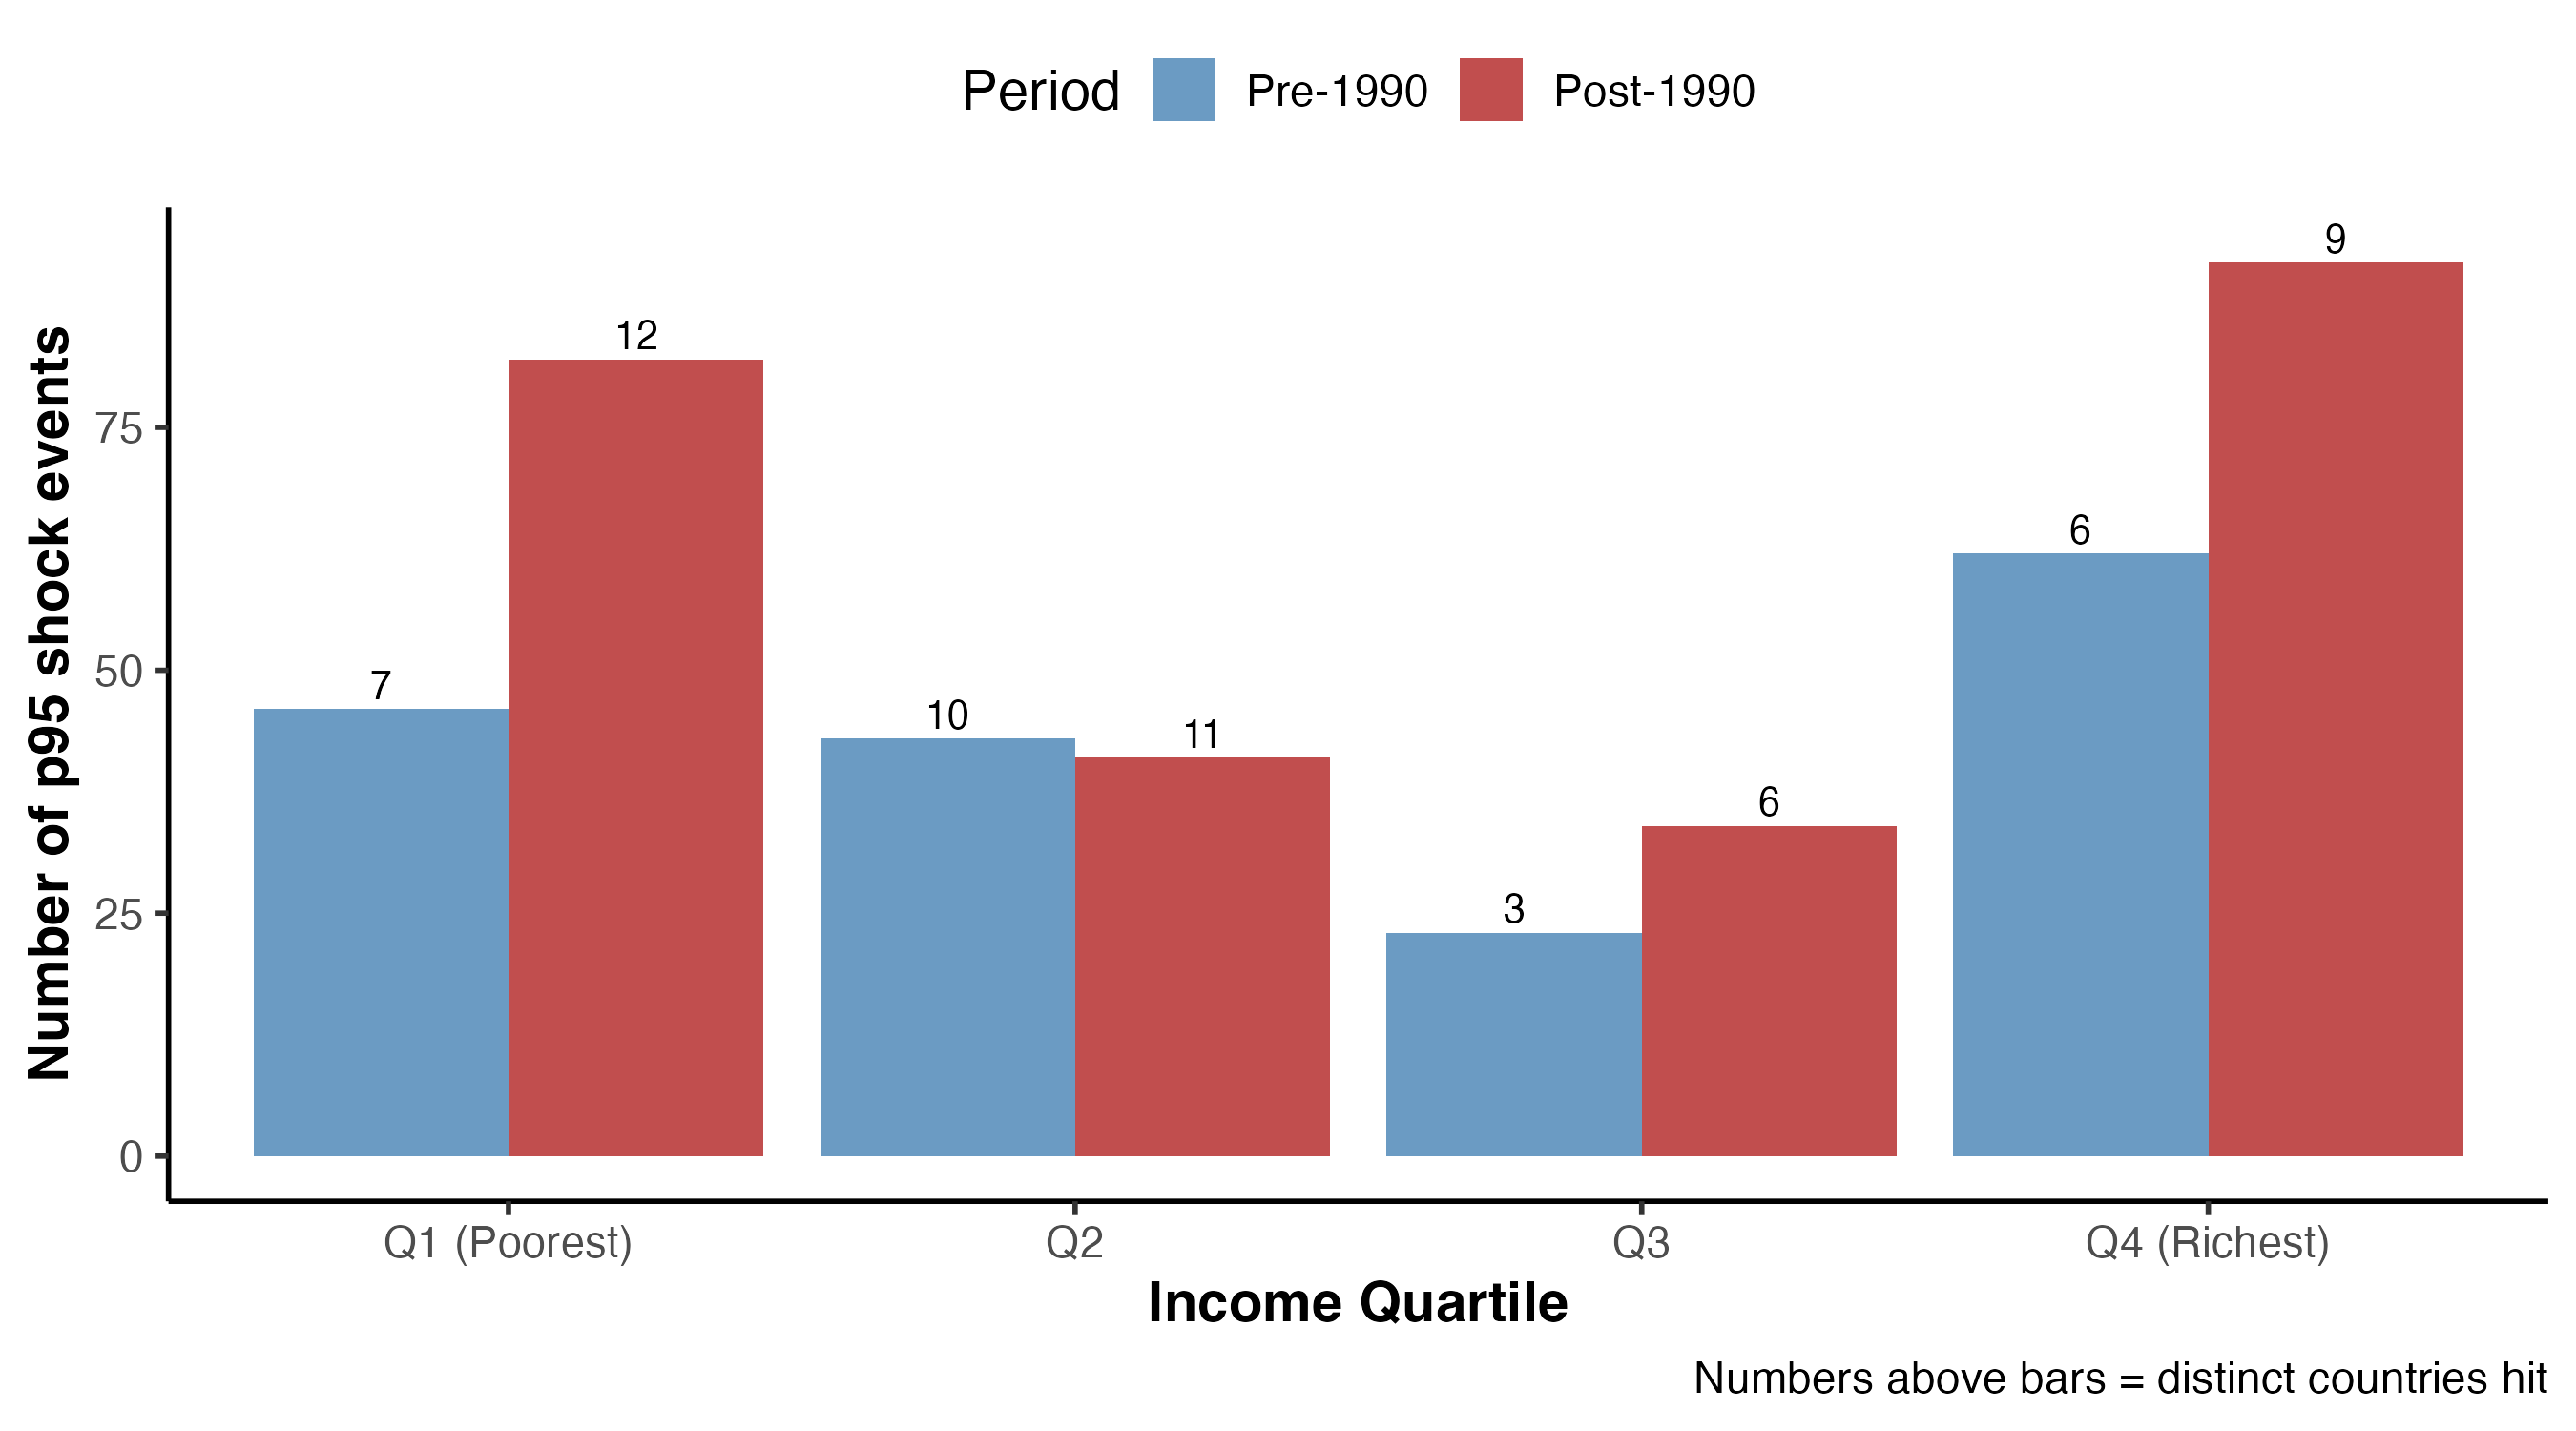
\includegraphics[width=0.85\textwidth,height=0.72\textheight,keepaspectratio]{figures/exposure_composition_by_income.png}

\smallskip
24 countries hit in both periods; 14 hit only post-1990. The identifying variation is \textbf{not constant}.
\end{frame}

\begin{frame}{High vs.\ Low Income: Period-Split IRFs}
\centering
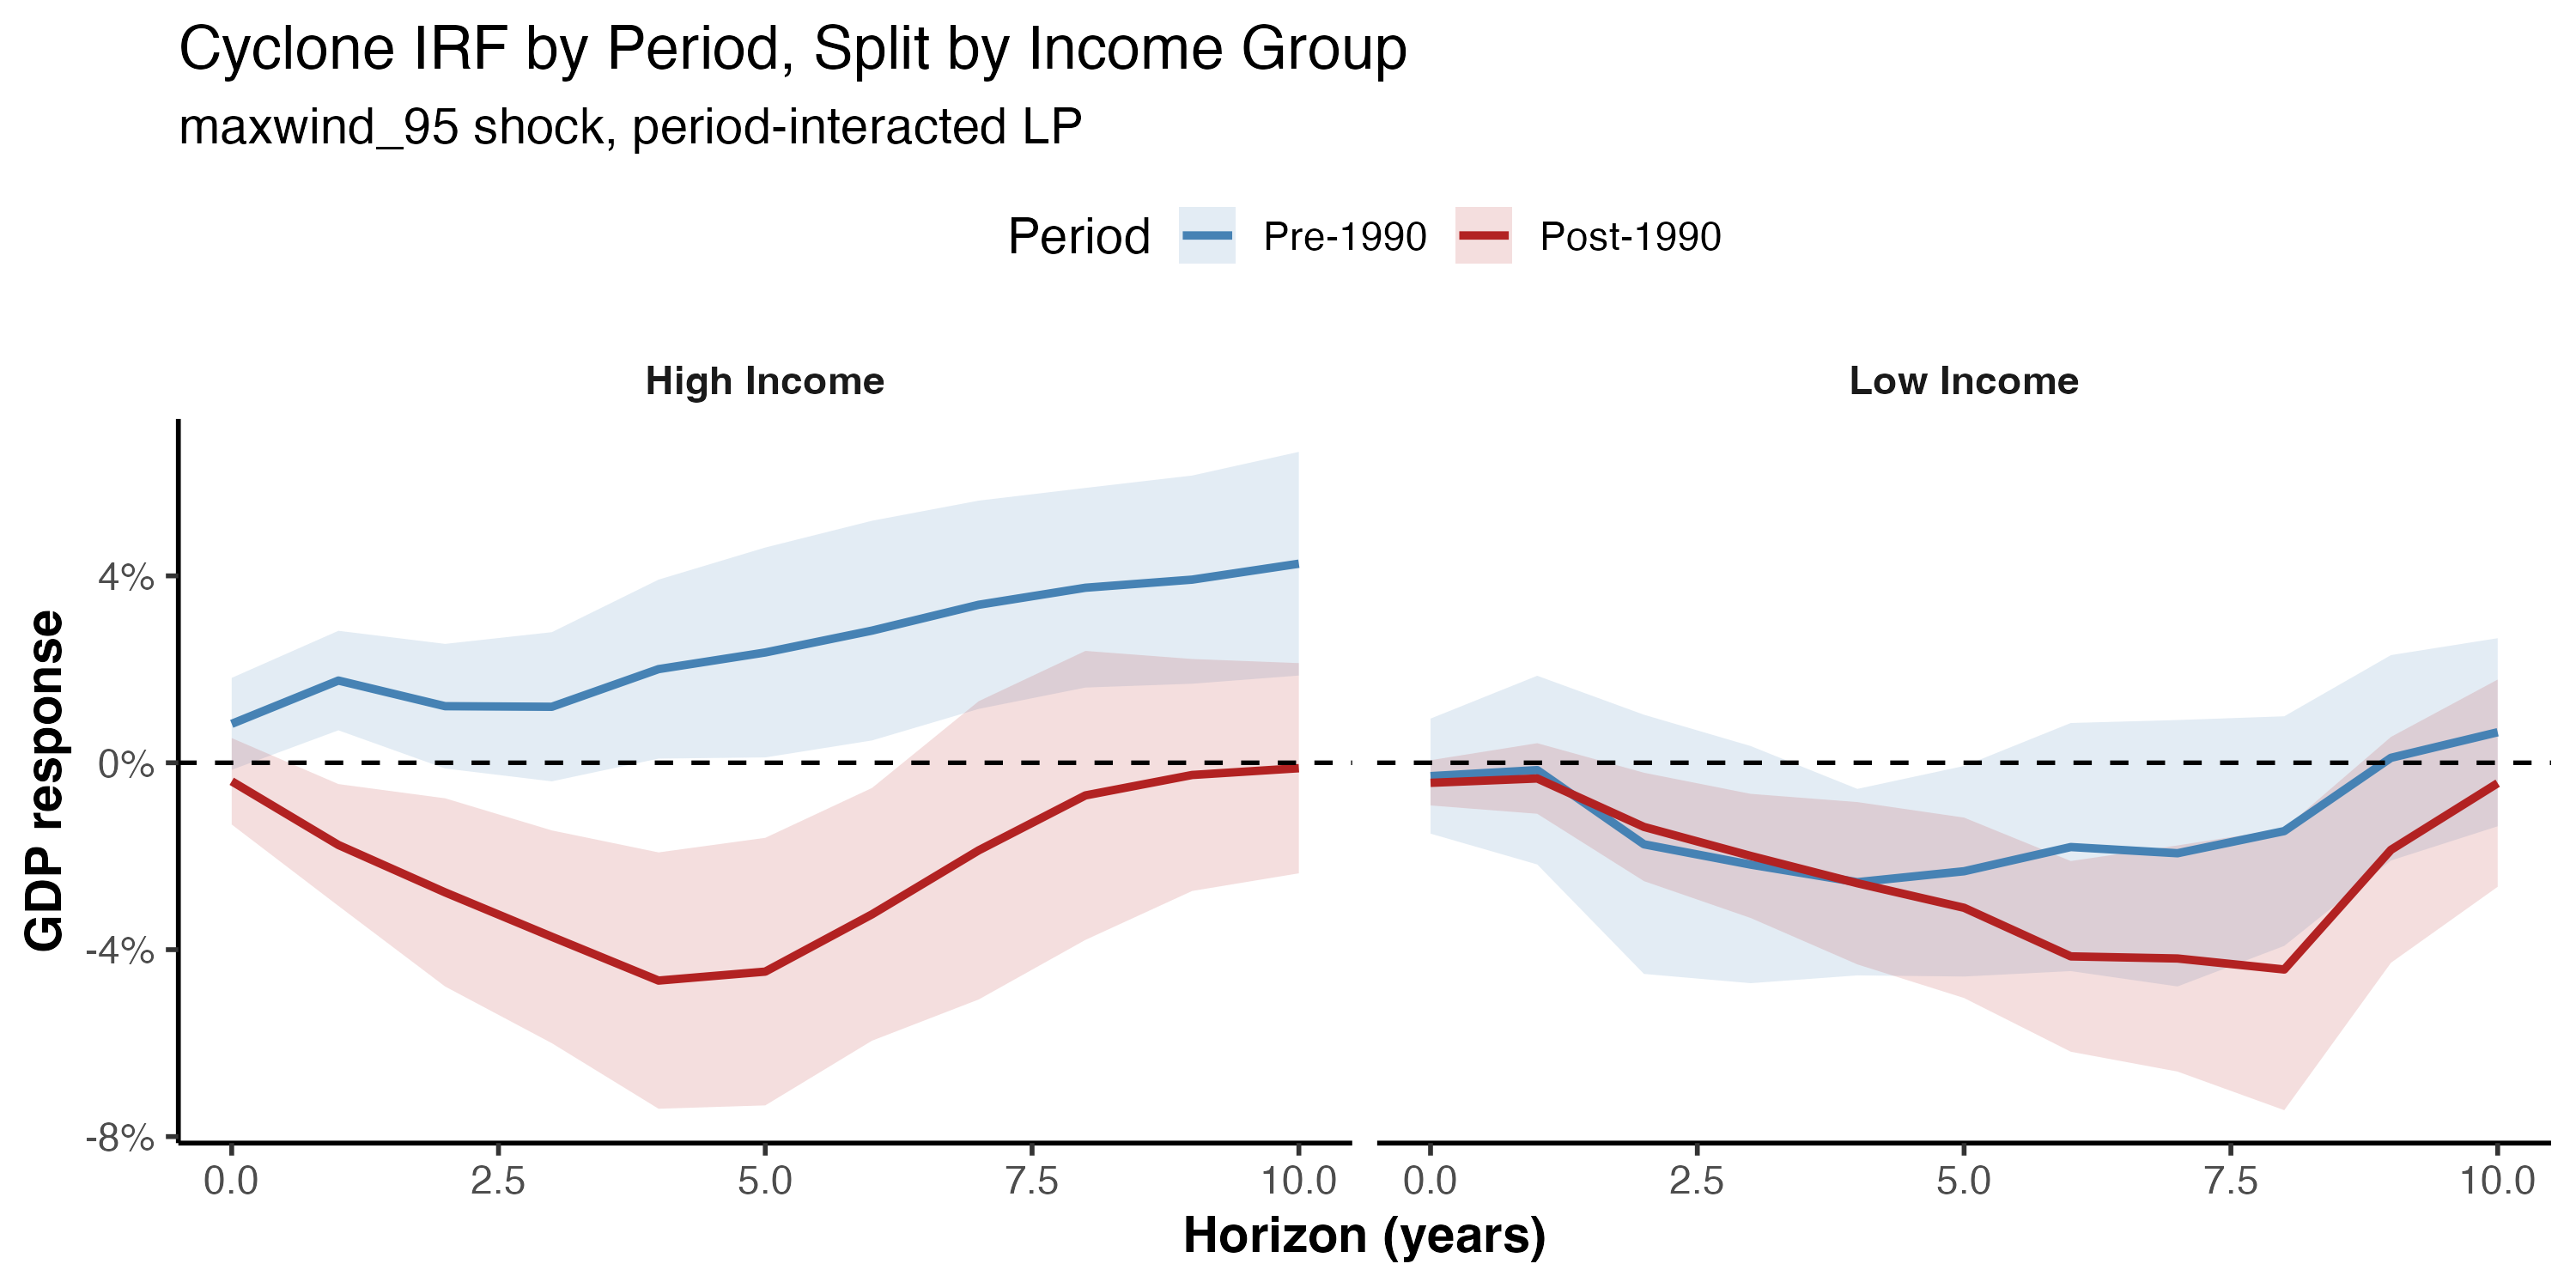
\includegraphics[width=\textwidth,height=0.78\textheight,keepaspectratio]{figures/vulnerability_irf_by_income_period.png}

The divergence is strongest for \textbf{high-income} countries.
\end{frame}

% - - - - - - - - - - - - - - - - - - - - - - - - - - - - - - -
\subsection{Structural Channels}
% - - - - - - - - - - - - - - - - - - - - - - - - - - - - - - -

{\hideframenumber
\begin{frame}
\subsectionpage
\end{frame}
\showframenumber}

\begin{frame}{Time Trend Interaction}
\centering
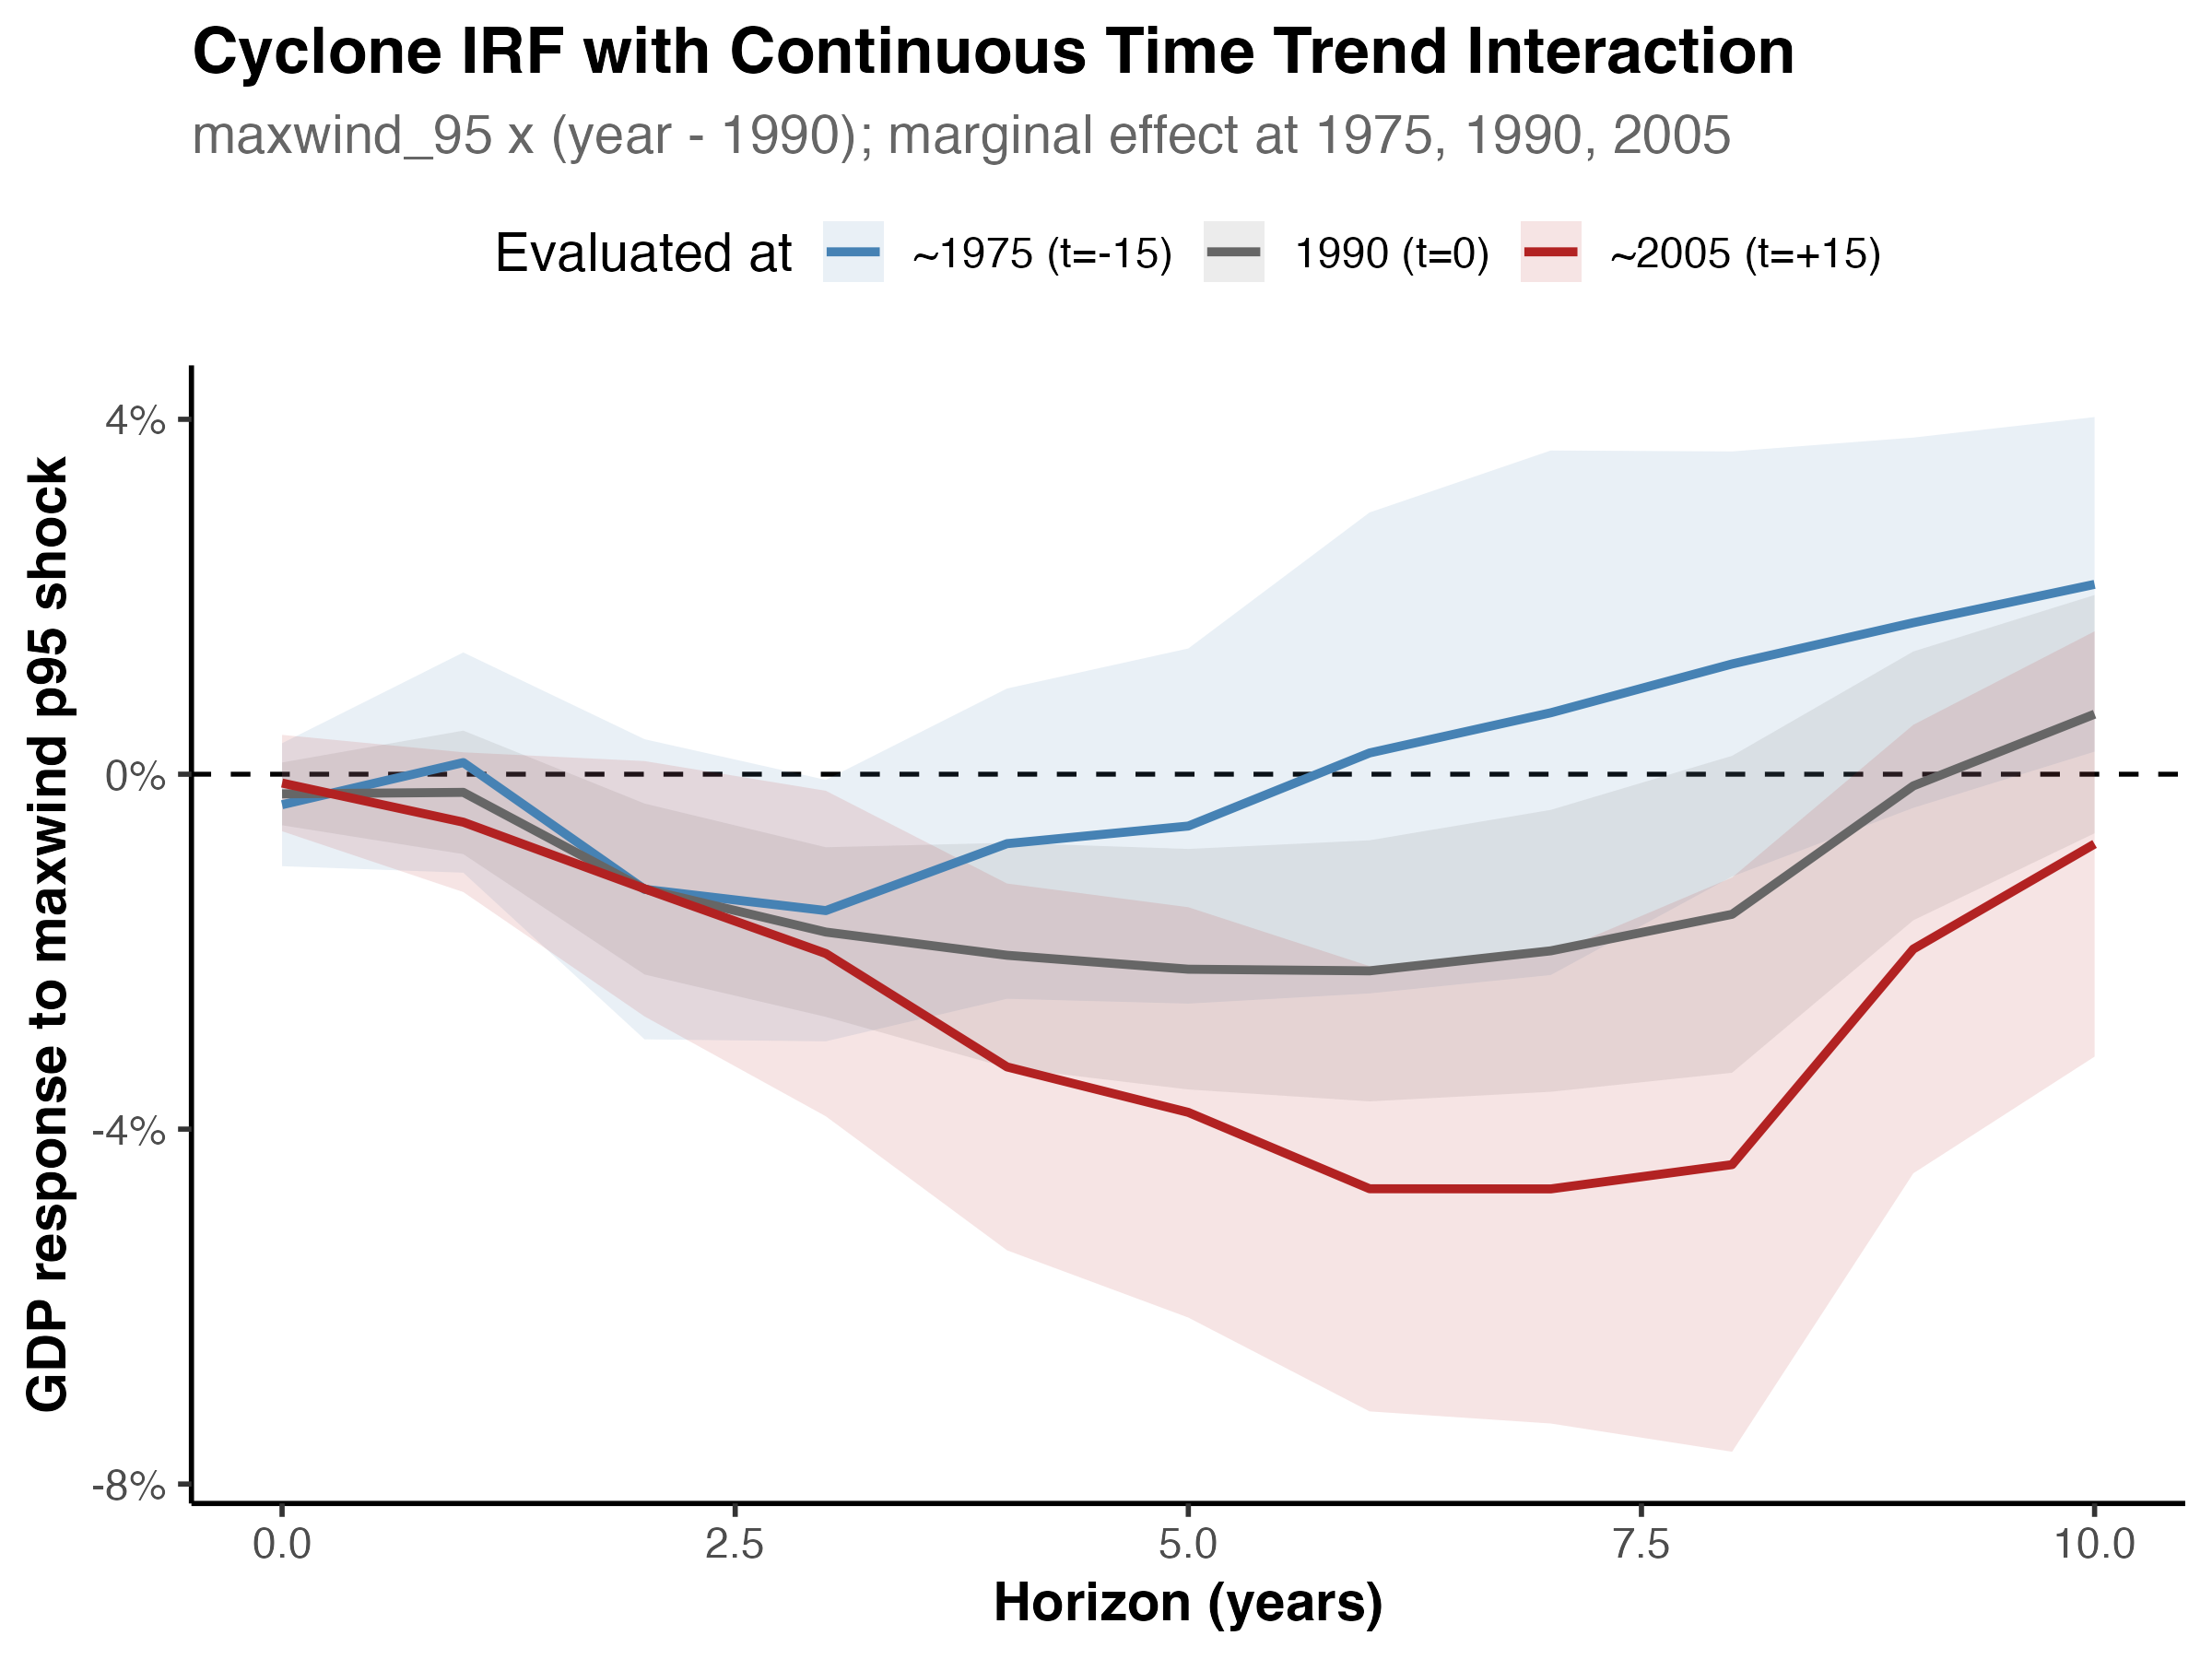
\includegraphics[width=0.75\textwidth,height=0.72\textheight,keepaspectratio]{figures/irf_time_trend.png}

Interacting the shock with $(year - 1990)$: the IRF deteriorates monotonically from near-zero in 1975 to $-6\%$ by 2005.
\end{frame}

\begin{frame}{Capital Intensity Interaction}
\centering
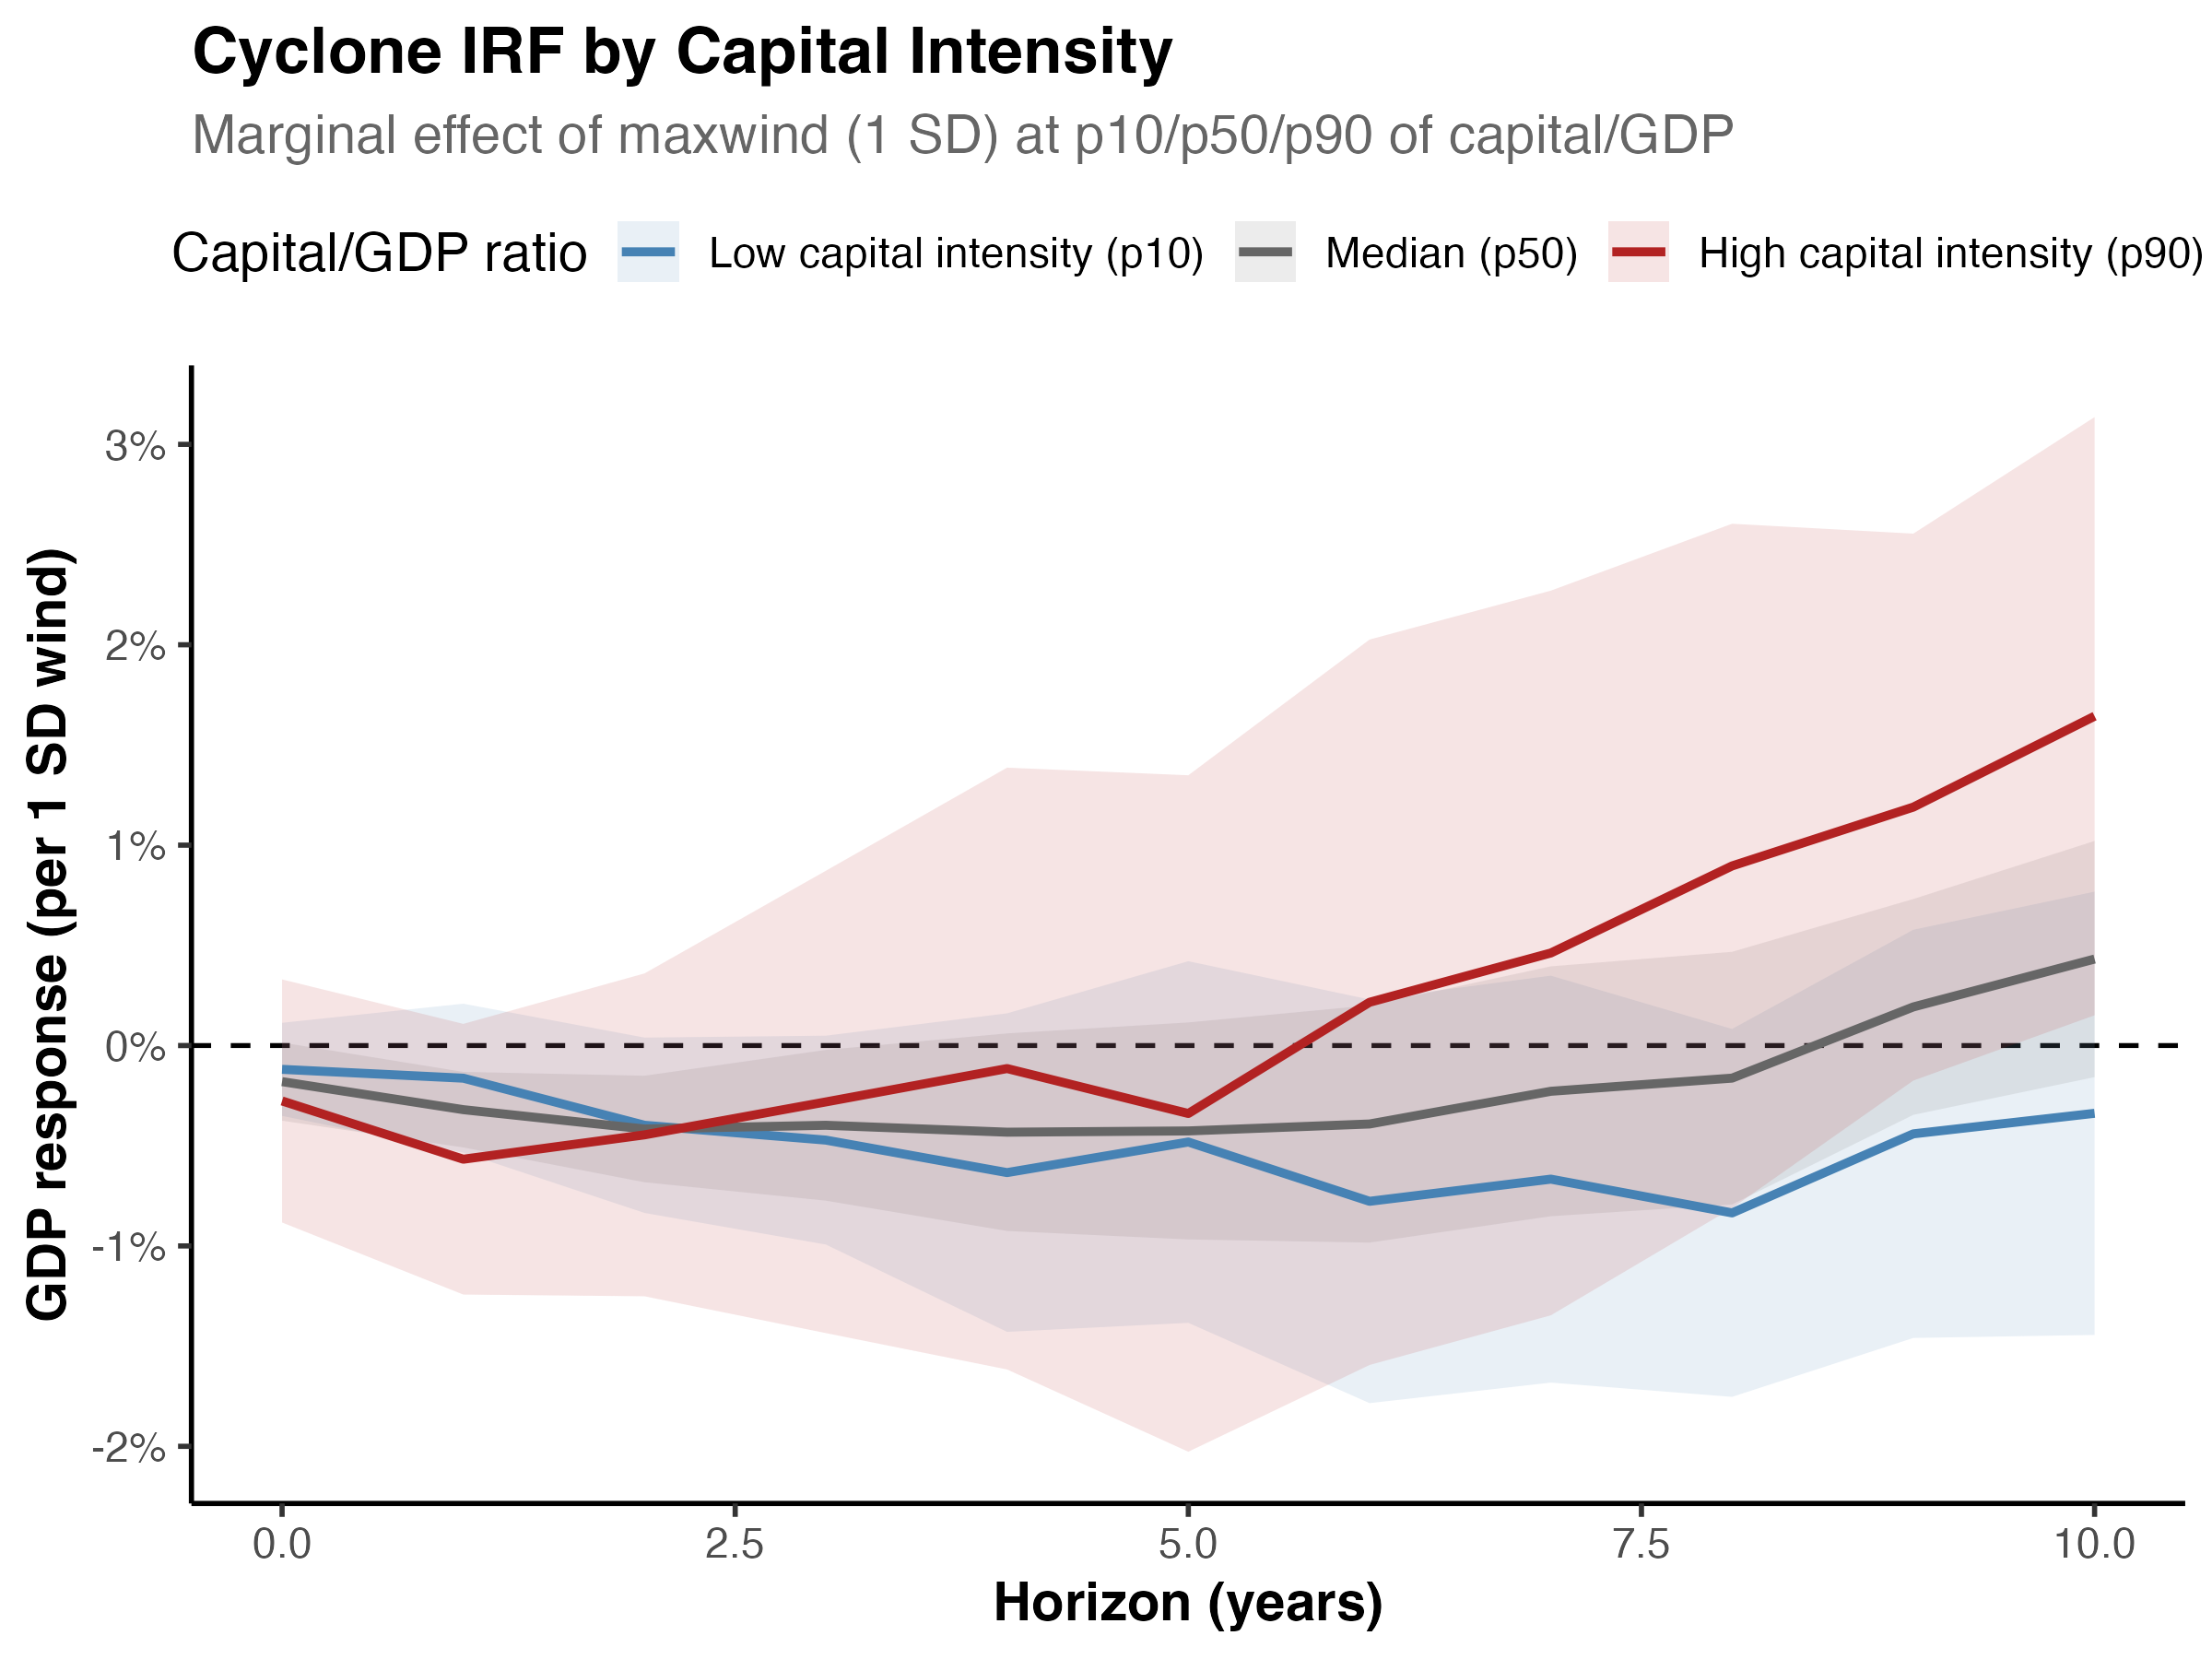
\includegraphics[width=0.75\textwidth,height=0.72\textheight,keepaspectratio]{figures/irf_capital_intensity.png}

High capital/GDP countries recover better. Low-capital countries suffer persistent losses.
\end{frame}

\begin{frame}{Human Capital Interaction}
\centering
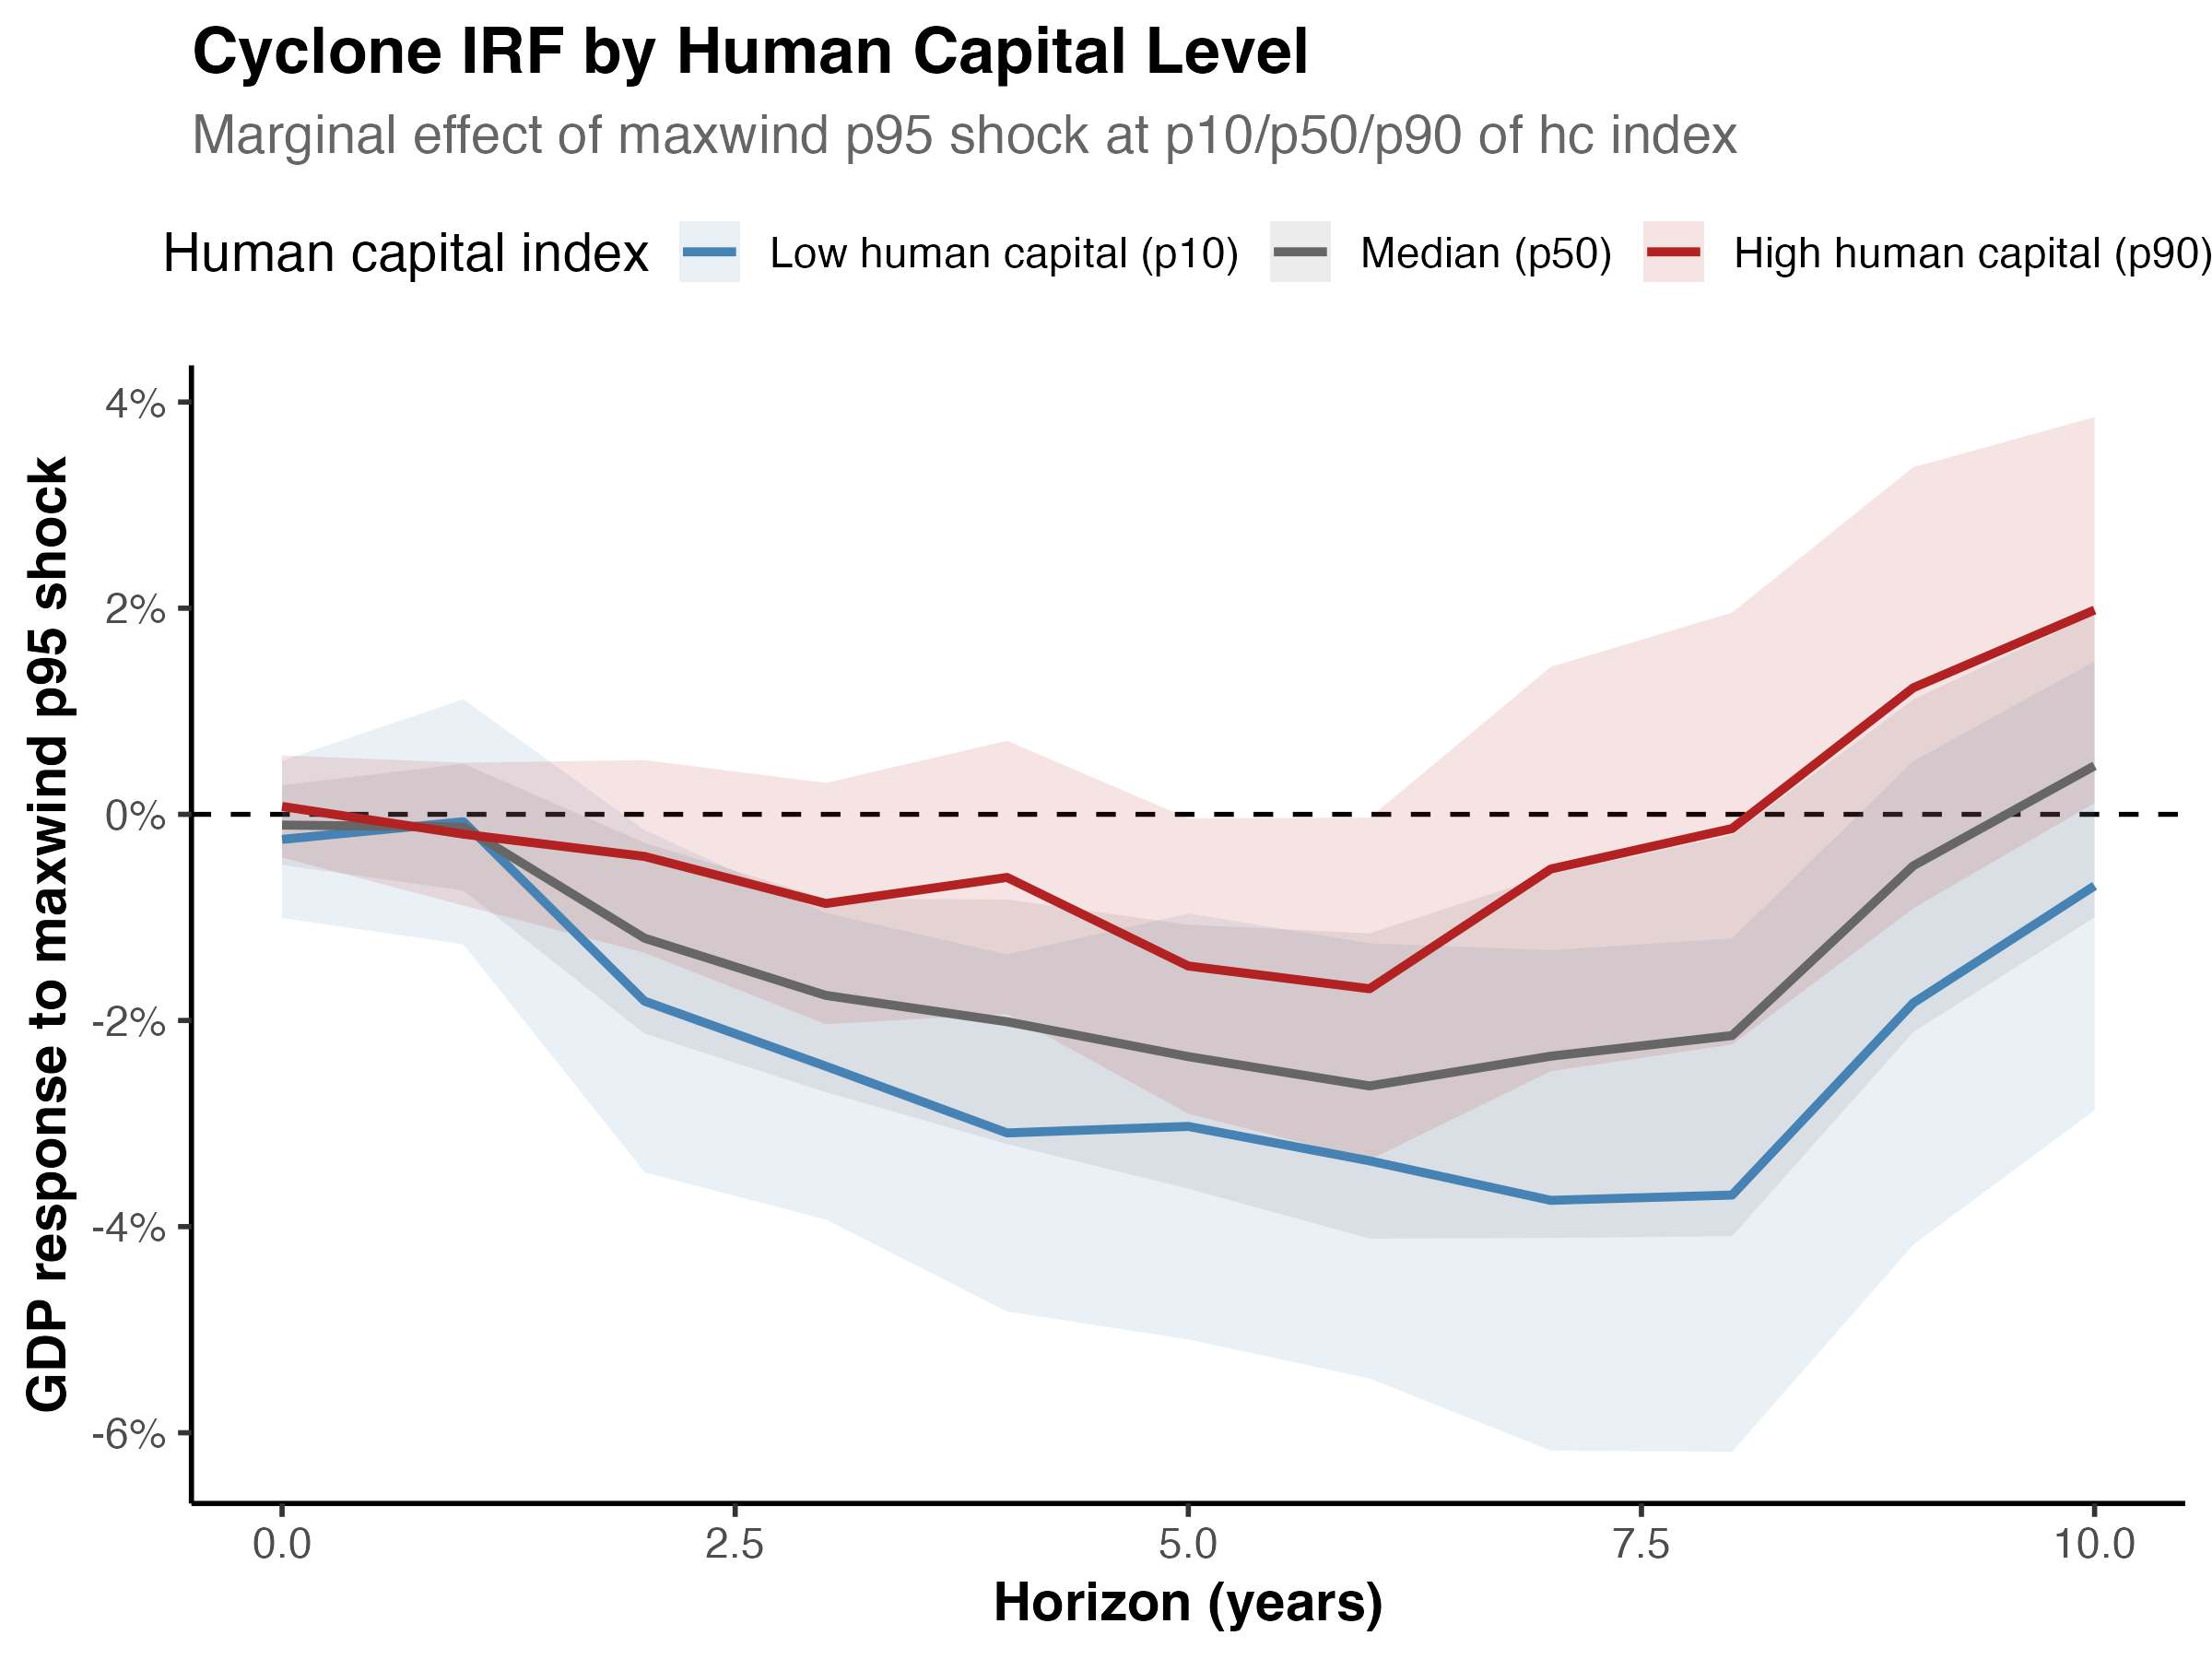
\includegraphics[width=0.75\textwidth,height=0.72\textheight,keepaspectratio]{figures/irf_human_capital.png}

Shock $\times$ PWT human capital index (demeaned); marginal effect at p10/p50/p90 via delta method. High HC enables recovery; low HC shows persistent $-3\%$ to $-5\%$ losses.
\end{frame}

\begin{frame}{Trade Openness and Investment Share}
\centering
\begin{columns}[T]
\column{0.48\textwidth}
\centering
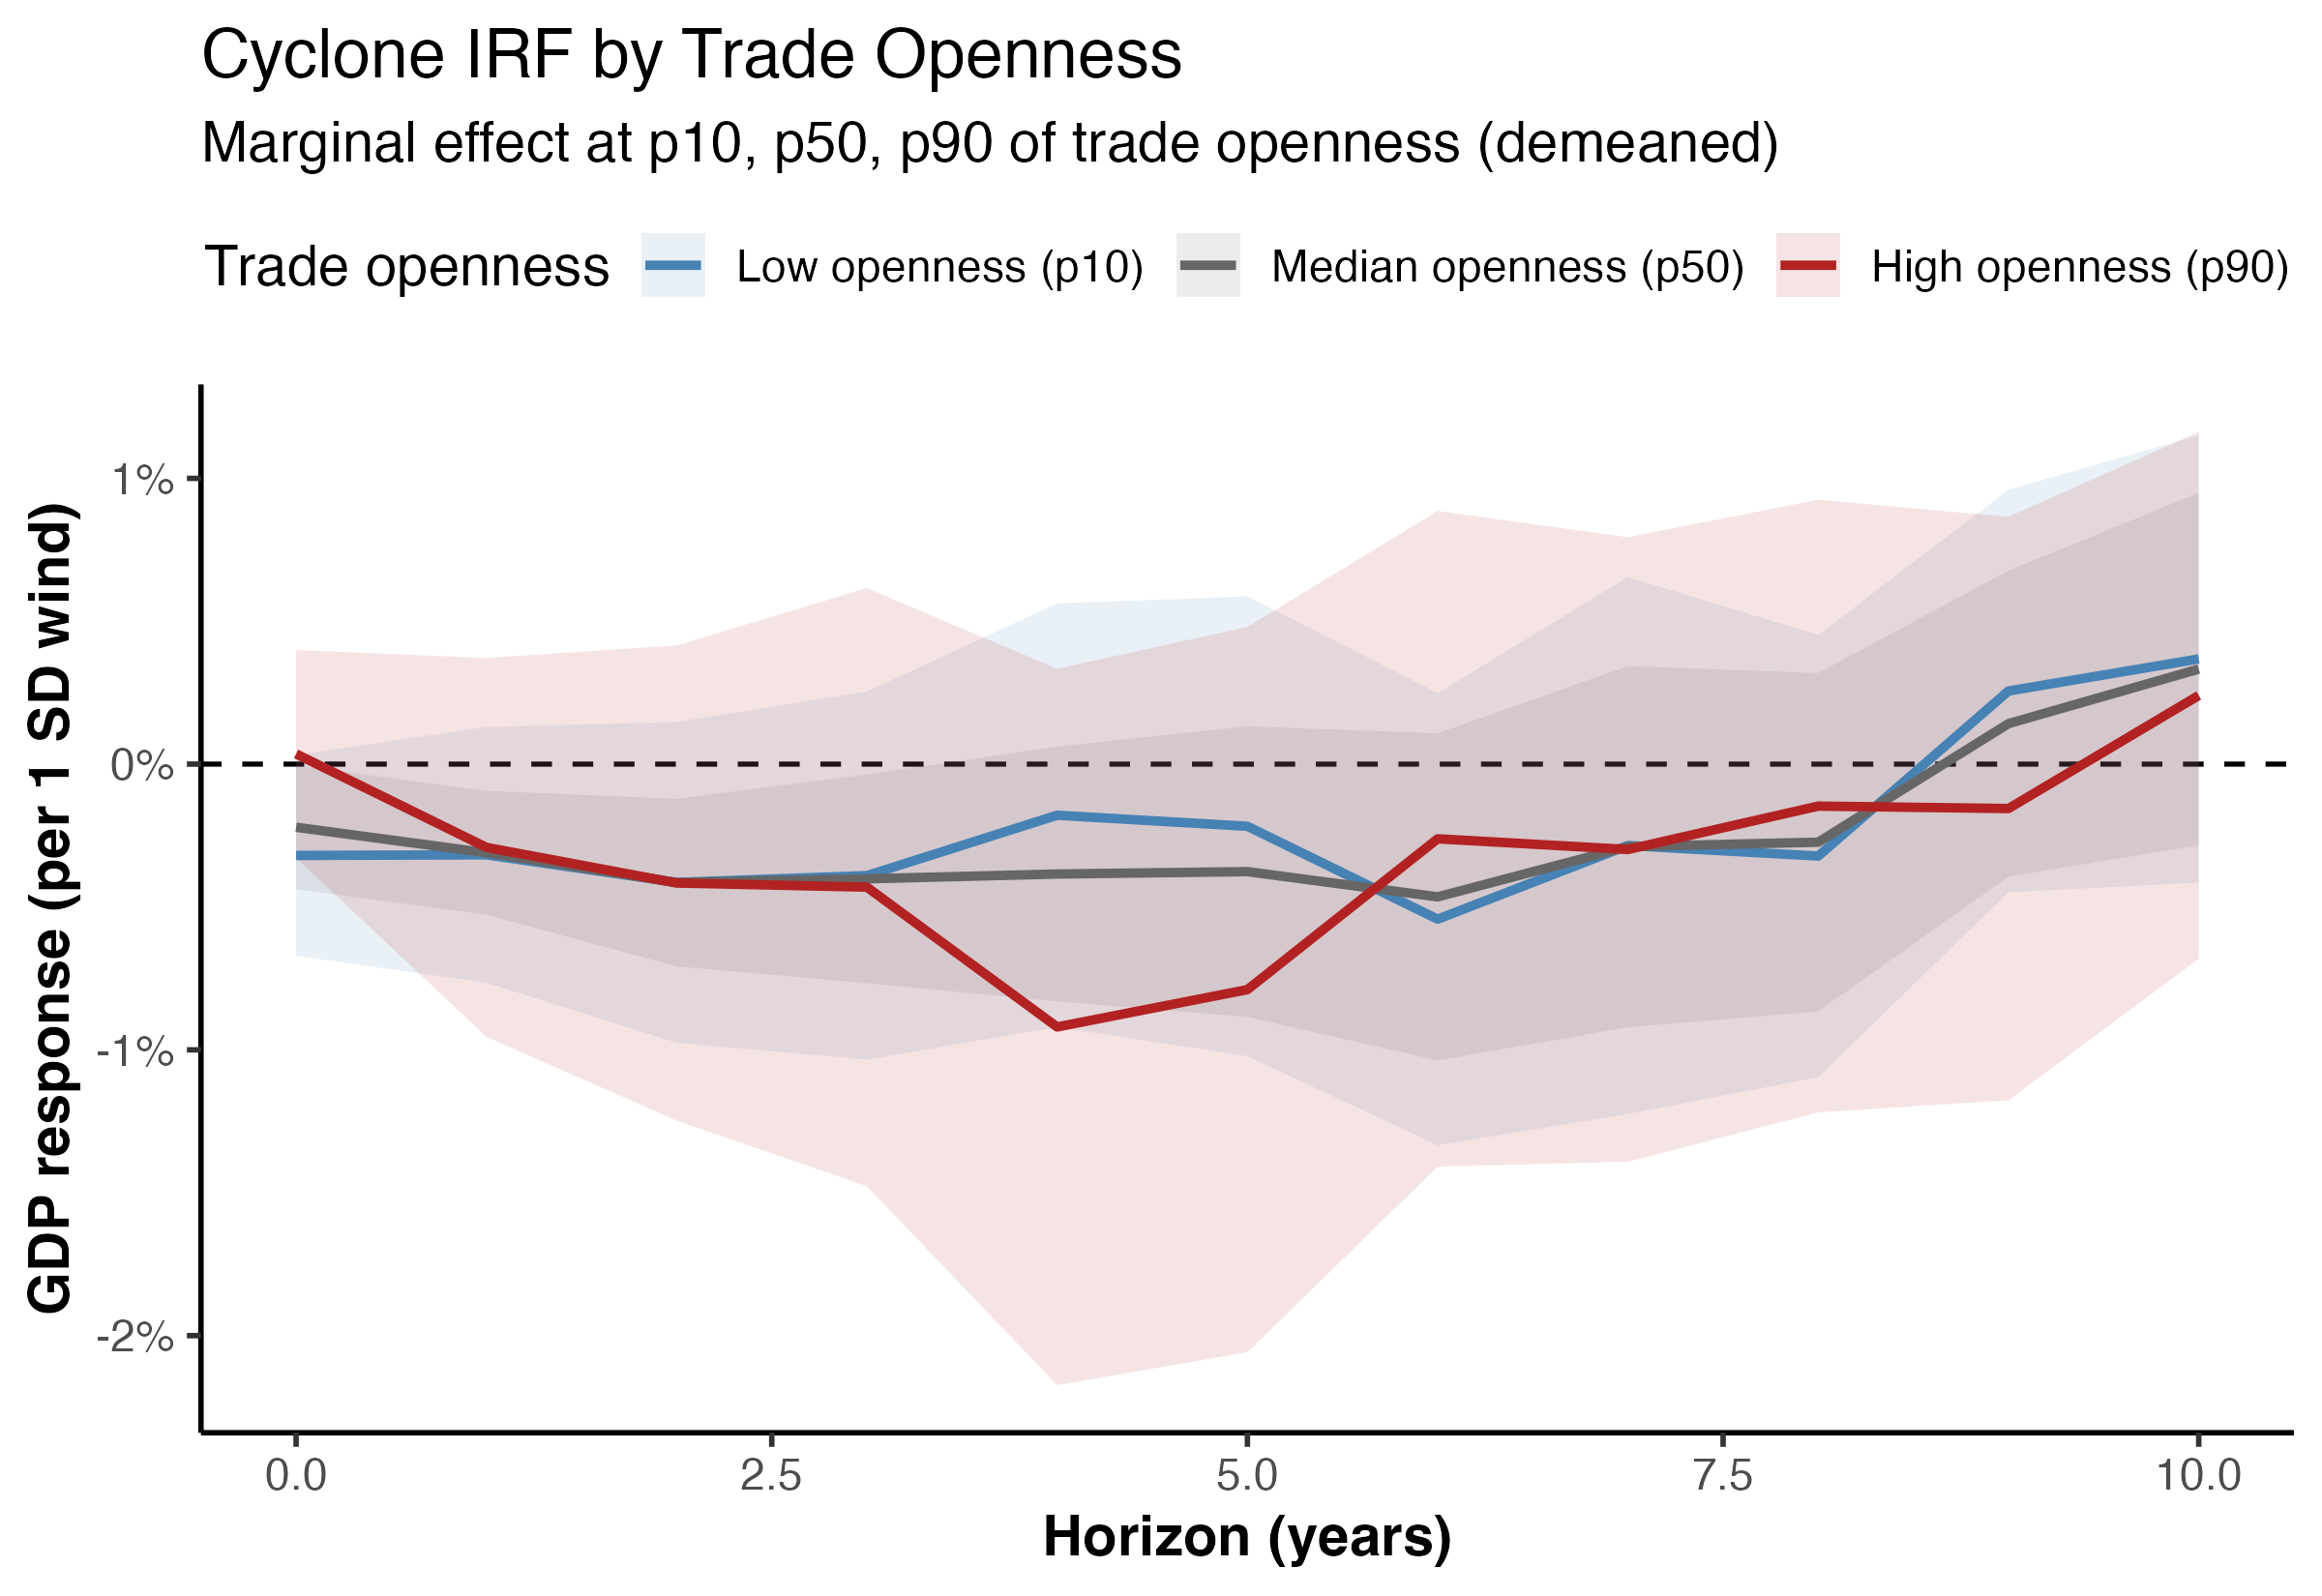
\includegraphics[width=\textwidth,height=0.60\textheight,keepaspectratio]{figures/irf_trade_openness.png}

\smallskip
{\small Trade: modest differentiation, CIs overlap.}

\column{0.48\textwidth}
\centering
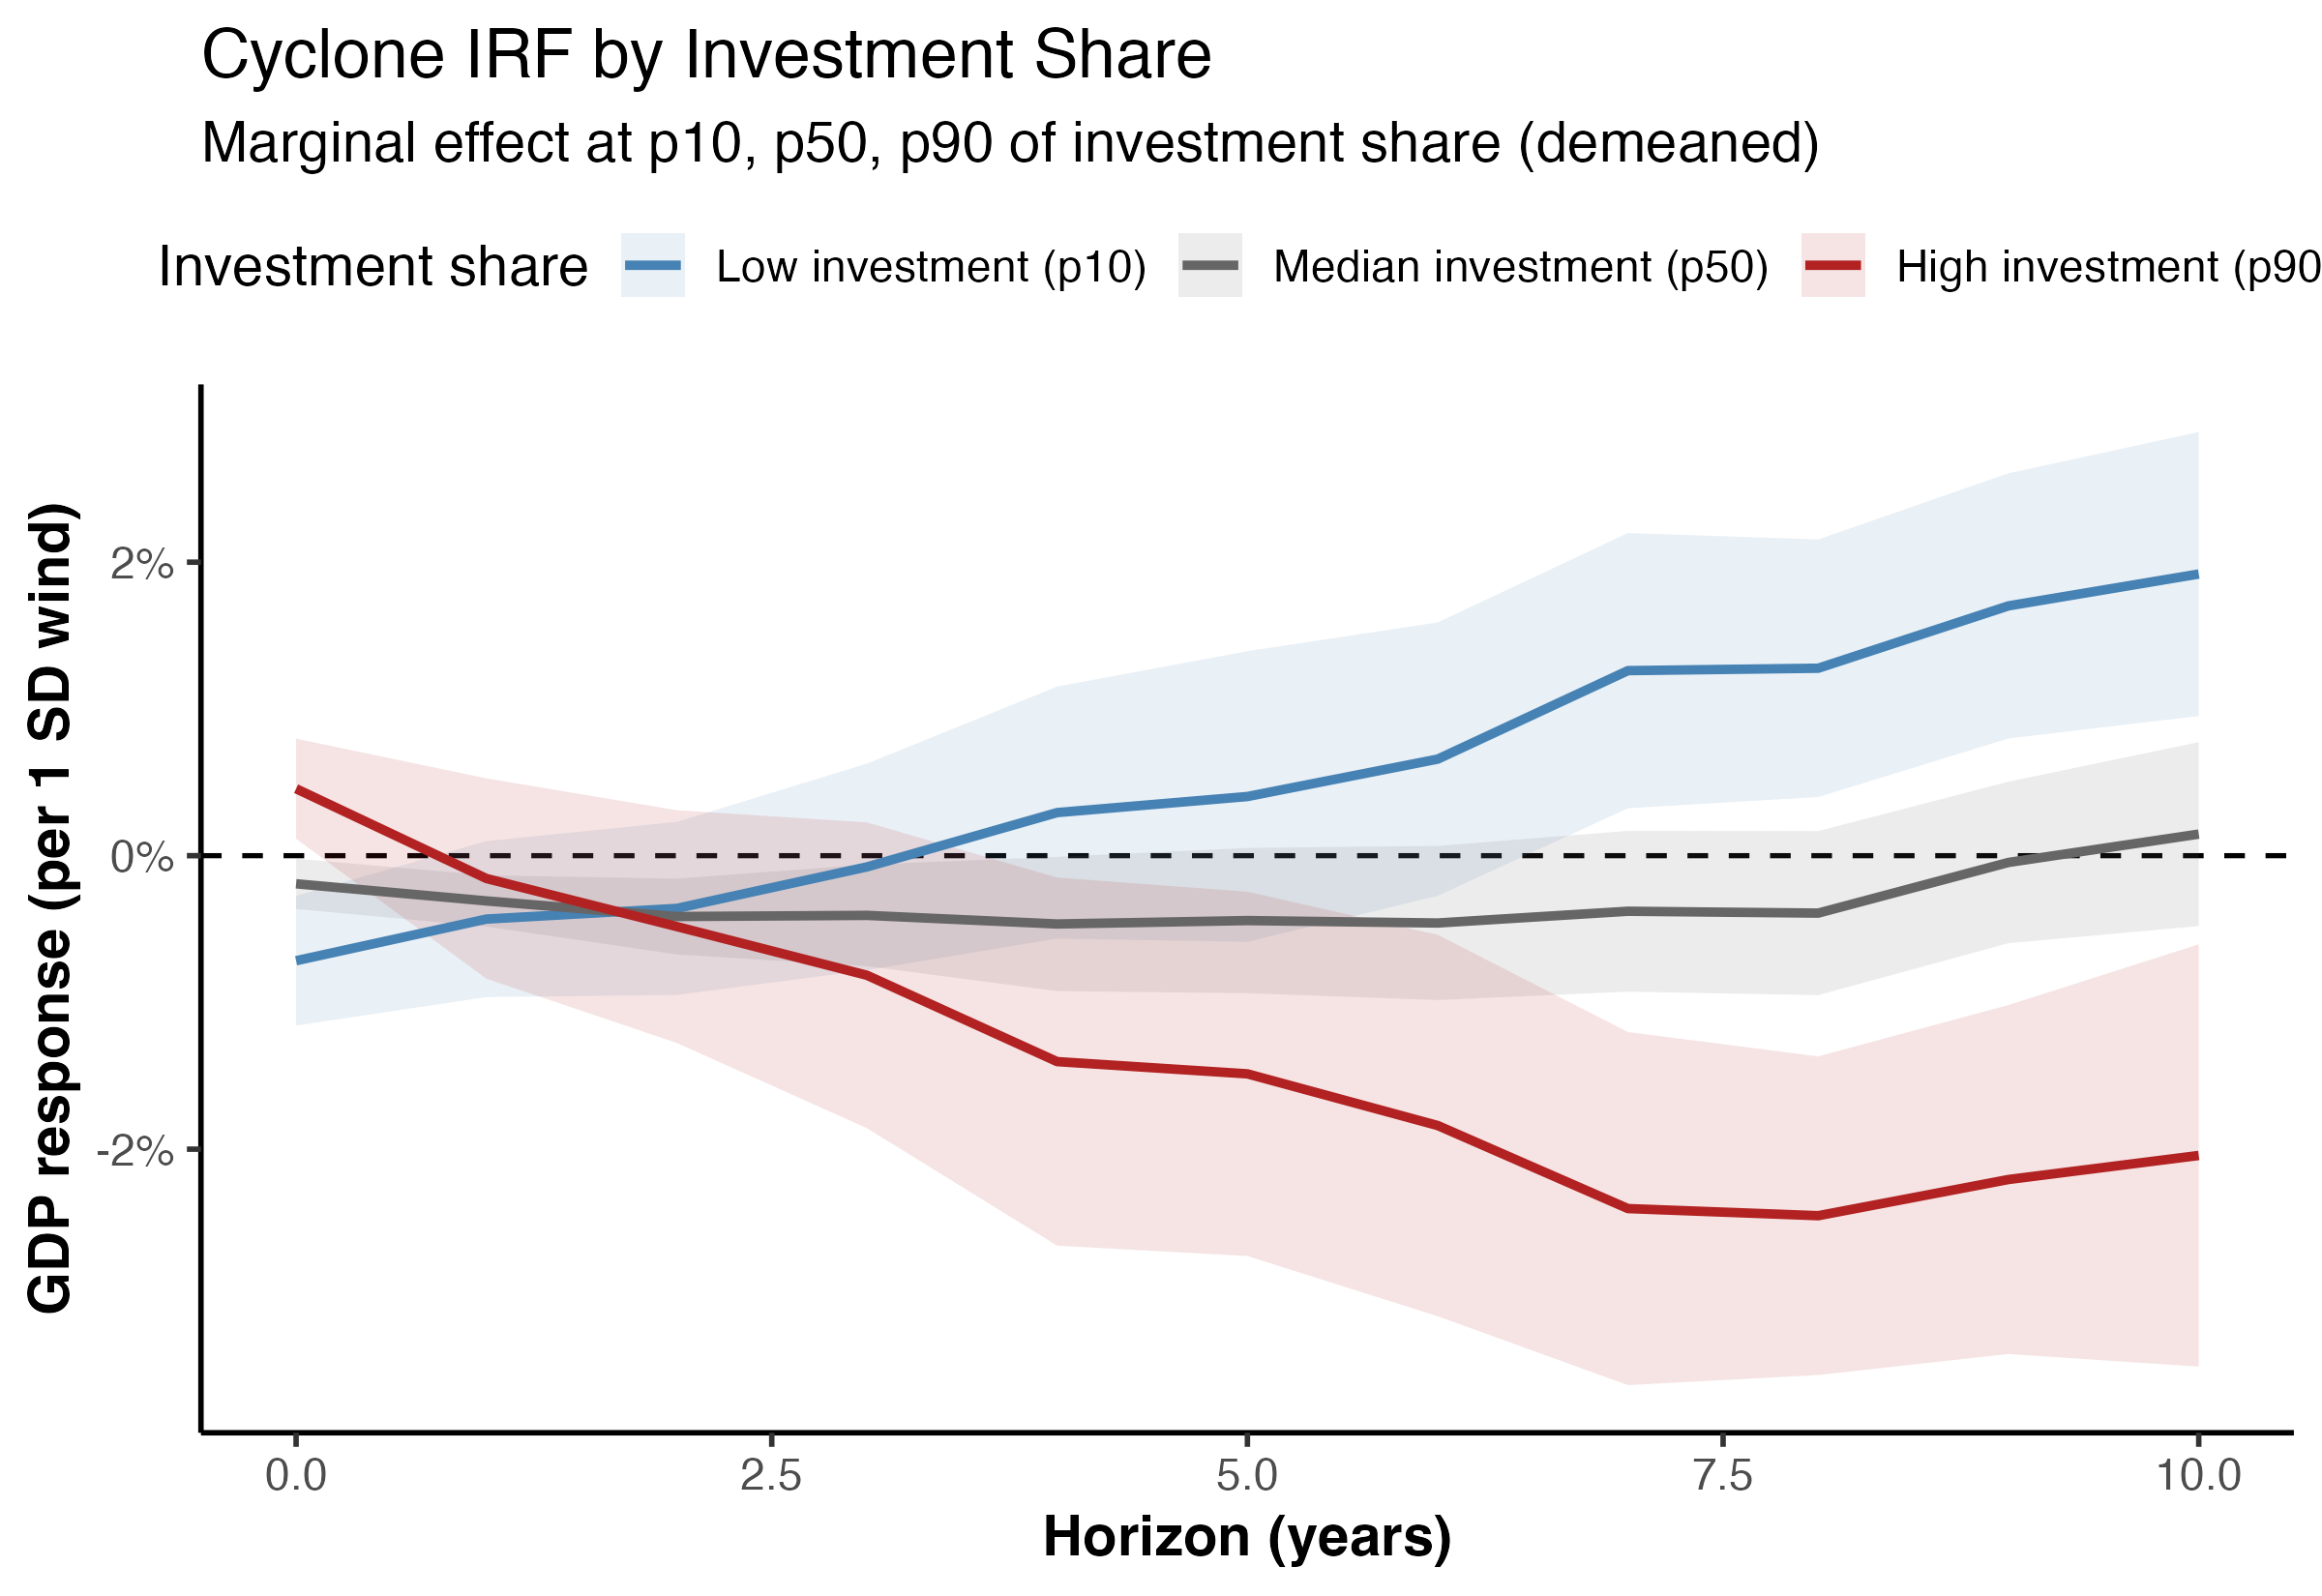
\includegraphics[width=\textwidth,height=0.60\textheight,keepaspectratio]{figures/irf_investment_share.png}

\smallskip
{\small Investment: strong cross-sectional predictor, but shares were stable across periods.}
\end{columns}
\end{frame}

\begin{frame}{Trade Terciles by Period}
\centering
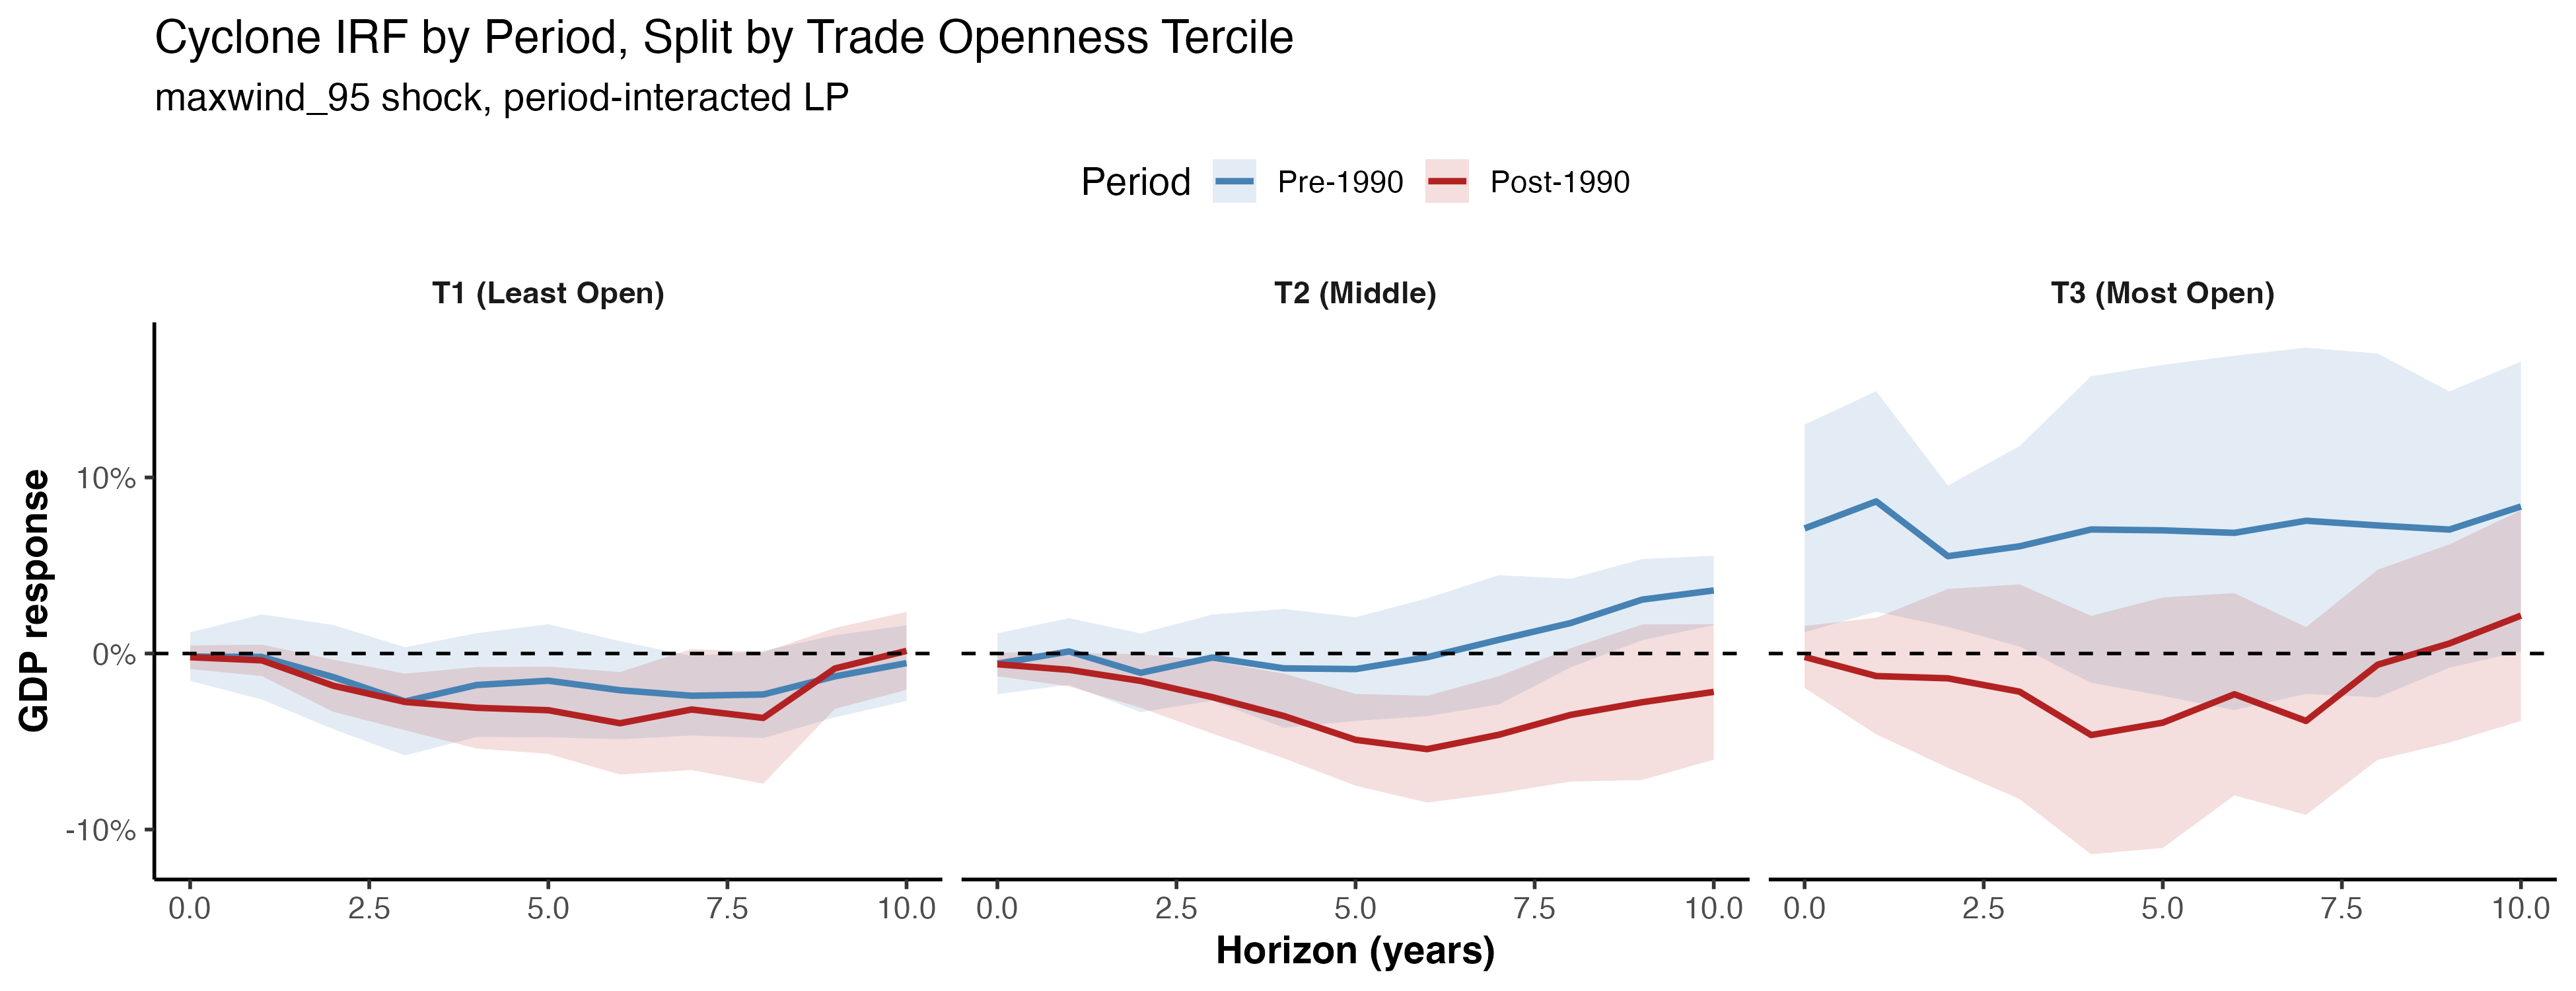
\includegraphics[width=\textwidth,height=0.72\textheight,keepaspectratio]{figures/irf_trade_terciles_by_period.png}

\smallskip
The pre/post divergence persists within all trade terciles. Trade openness does not explain it.
\end{frame}

\begin{frame}{Structural Channels: Summary}
\begin{itemize}
  \item \textbf{Time trend}: effect deteriorates monotonically (not a discrete break)
  \item \textbf{Capital and human capital}: predict cross-sectional recovery, but both \emph{improved} over time --- cannot explain temporal deterioration
  \item \textbf{Trade}: no significant interaction; divergence persists within all terciles
  \item \textbf{Investment}: strong predictor ($-4$pp spread), but shares were stable across periods
\end{itemize}
\bigskip
No single channel explains the temporal shift. So what does?
\end{frame}

% - - - - - - - - - - - - - - - - - - - - - - - - - - - - - - -
\subsection{The Control Group}
% - - - - - - - - - - - - - - - - - - - - - - - - - - - - - - -

{\hideframenumber
\begin{frame}
\subsectionpage
\end{frame}
\showframenumber}

\begin{frame}{The Control Group Problem}
In TWFE local projections, the year FE $\delta_t$ absorbs the \textbf{average GDP path} across all countries:
\[
  \hat{\delta}_t \;\approx\; \frac{1}{N}\sum_{i=1}^{N}\bigl(y_{i,t+h} - y_{i,t-1} - \hat{\gamma}'X_{it}\bigr)
\]

\begin{itemize}
  \item \textbf{142 of 182} countries never experience a p95 cyclone shock
  \item These countries \textbf{dominate} the year FE $\to$ they define the counterfactual
  \item Never-treated: \textbf{Europe} (37) and \textbf{Africa} (47)
  \item Cyclone-exposed: \textbf{Americas} (18) and \textbf{Asia} (15)
  \item If these regions have different GDP trends, the year FE absorbs the \emph{wrong} counterfactual
\end{itemize}
\end{frame}

\begin{frame}{GDP Trends: Treated vs.\ Never-Treated}
\centering
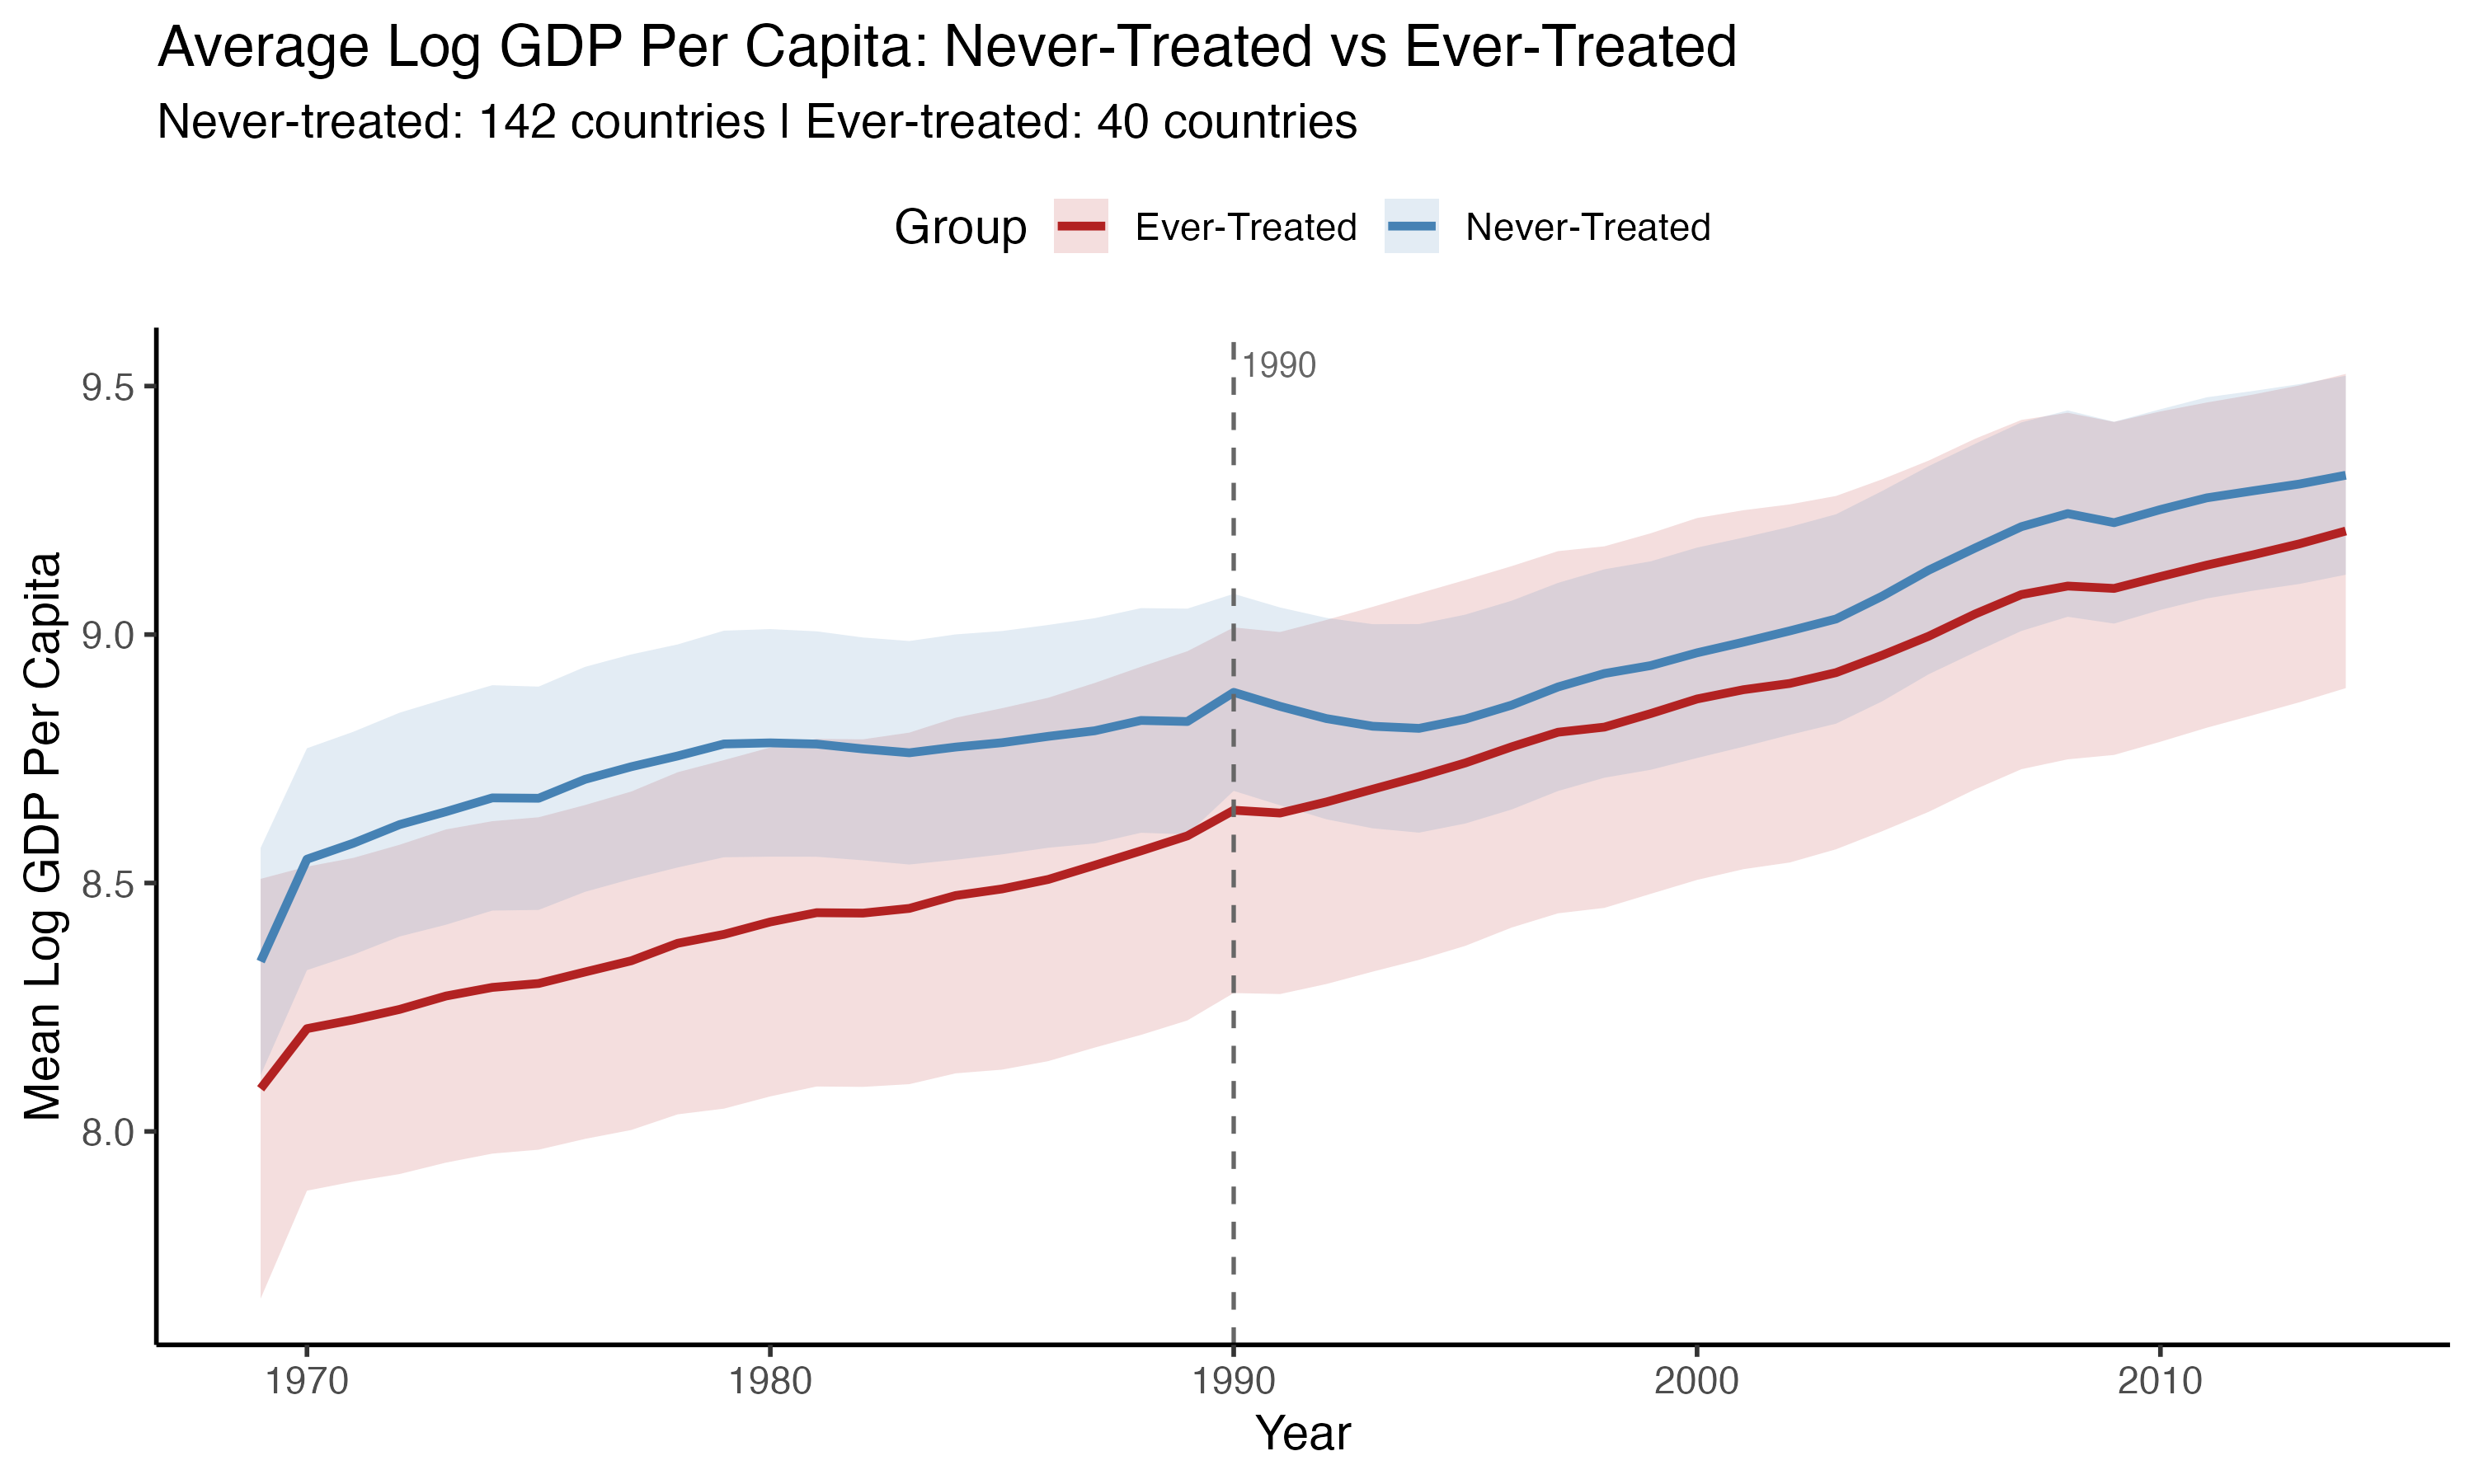
\includegraphics[width=0.85\textwidth,height=0.72\textheight,keepaspectratio]{figures/gdp_trends_treated_vs_untreated.png}

Never-treated countries have higher average GDP but similar growth. The control group shapes the year FE.
\end{frame}

\begin{frame}{Dropping Never-Treated Countries}
\centering
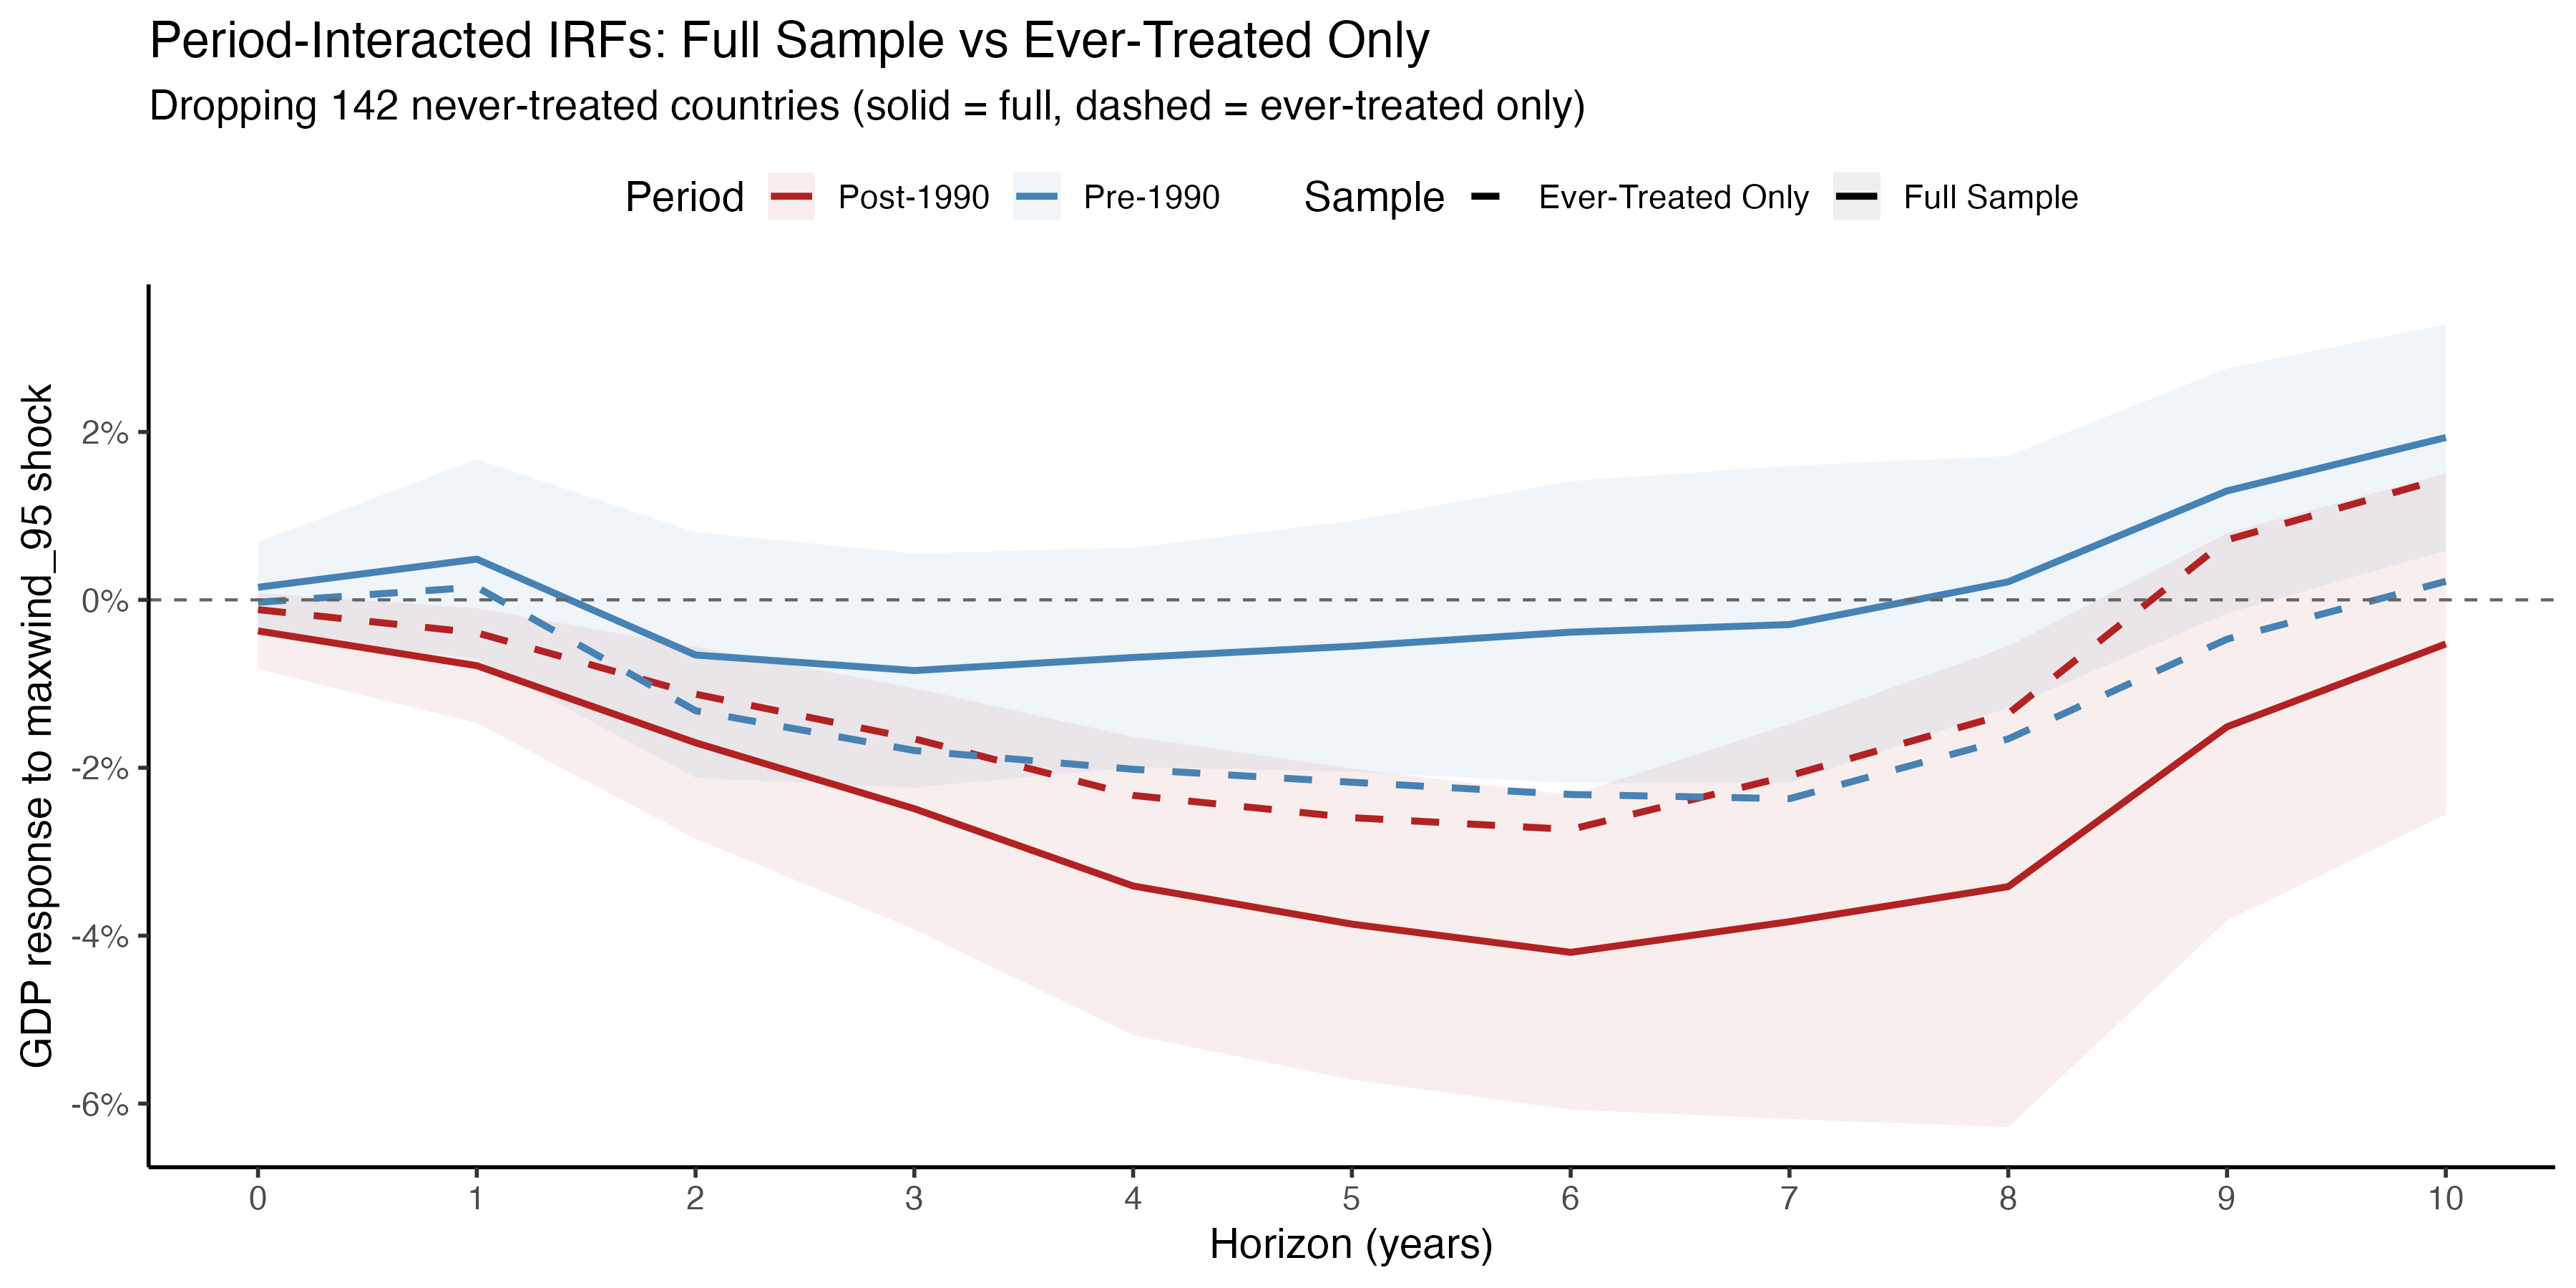
\includegraphics[width=\textwidth,height=0.68\textheight,keepaspectratio]{figures/irf_drop_never_treated.png}

\smallskip
Dropping 142 never-treated countries: post-1990 effect attenuates from $-3.9\%$ to $-2.6\%$ at $h = 5$.
\end{frame}

\begin{frame}{Varying Sample Restrictions}
\centering
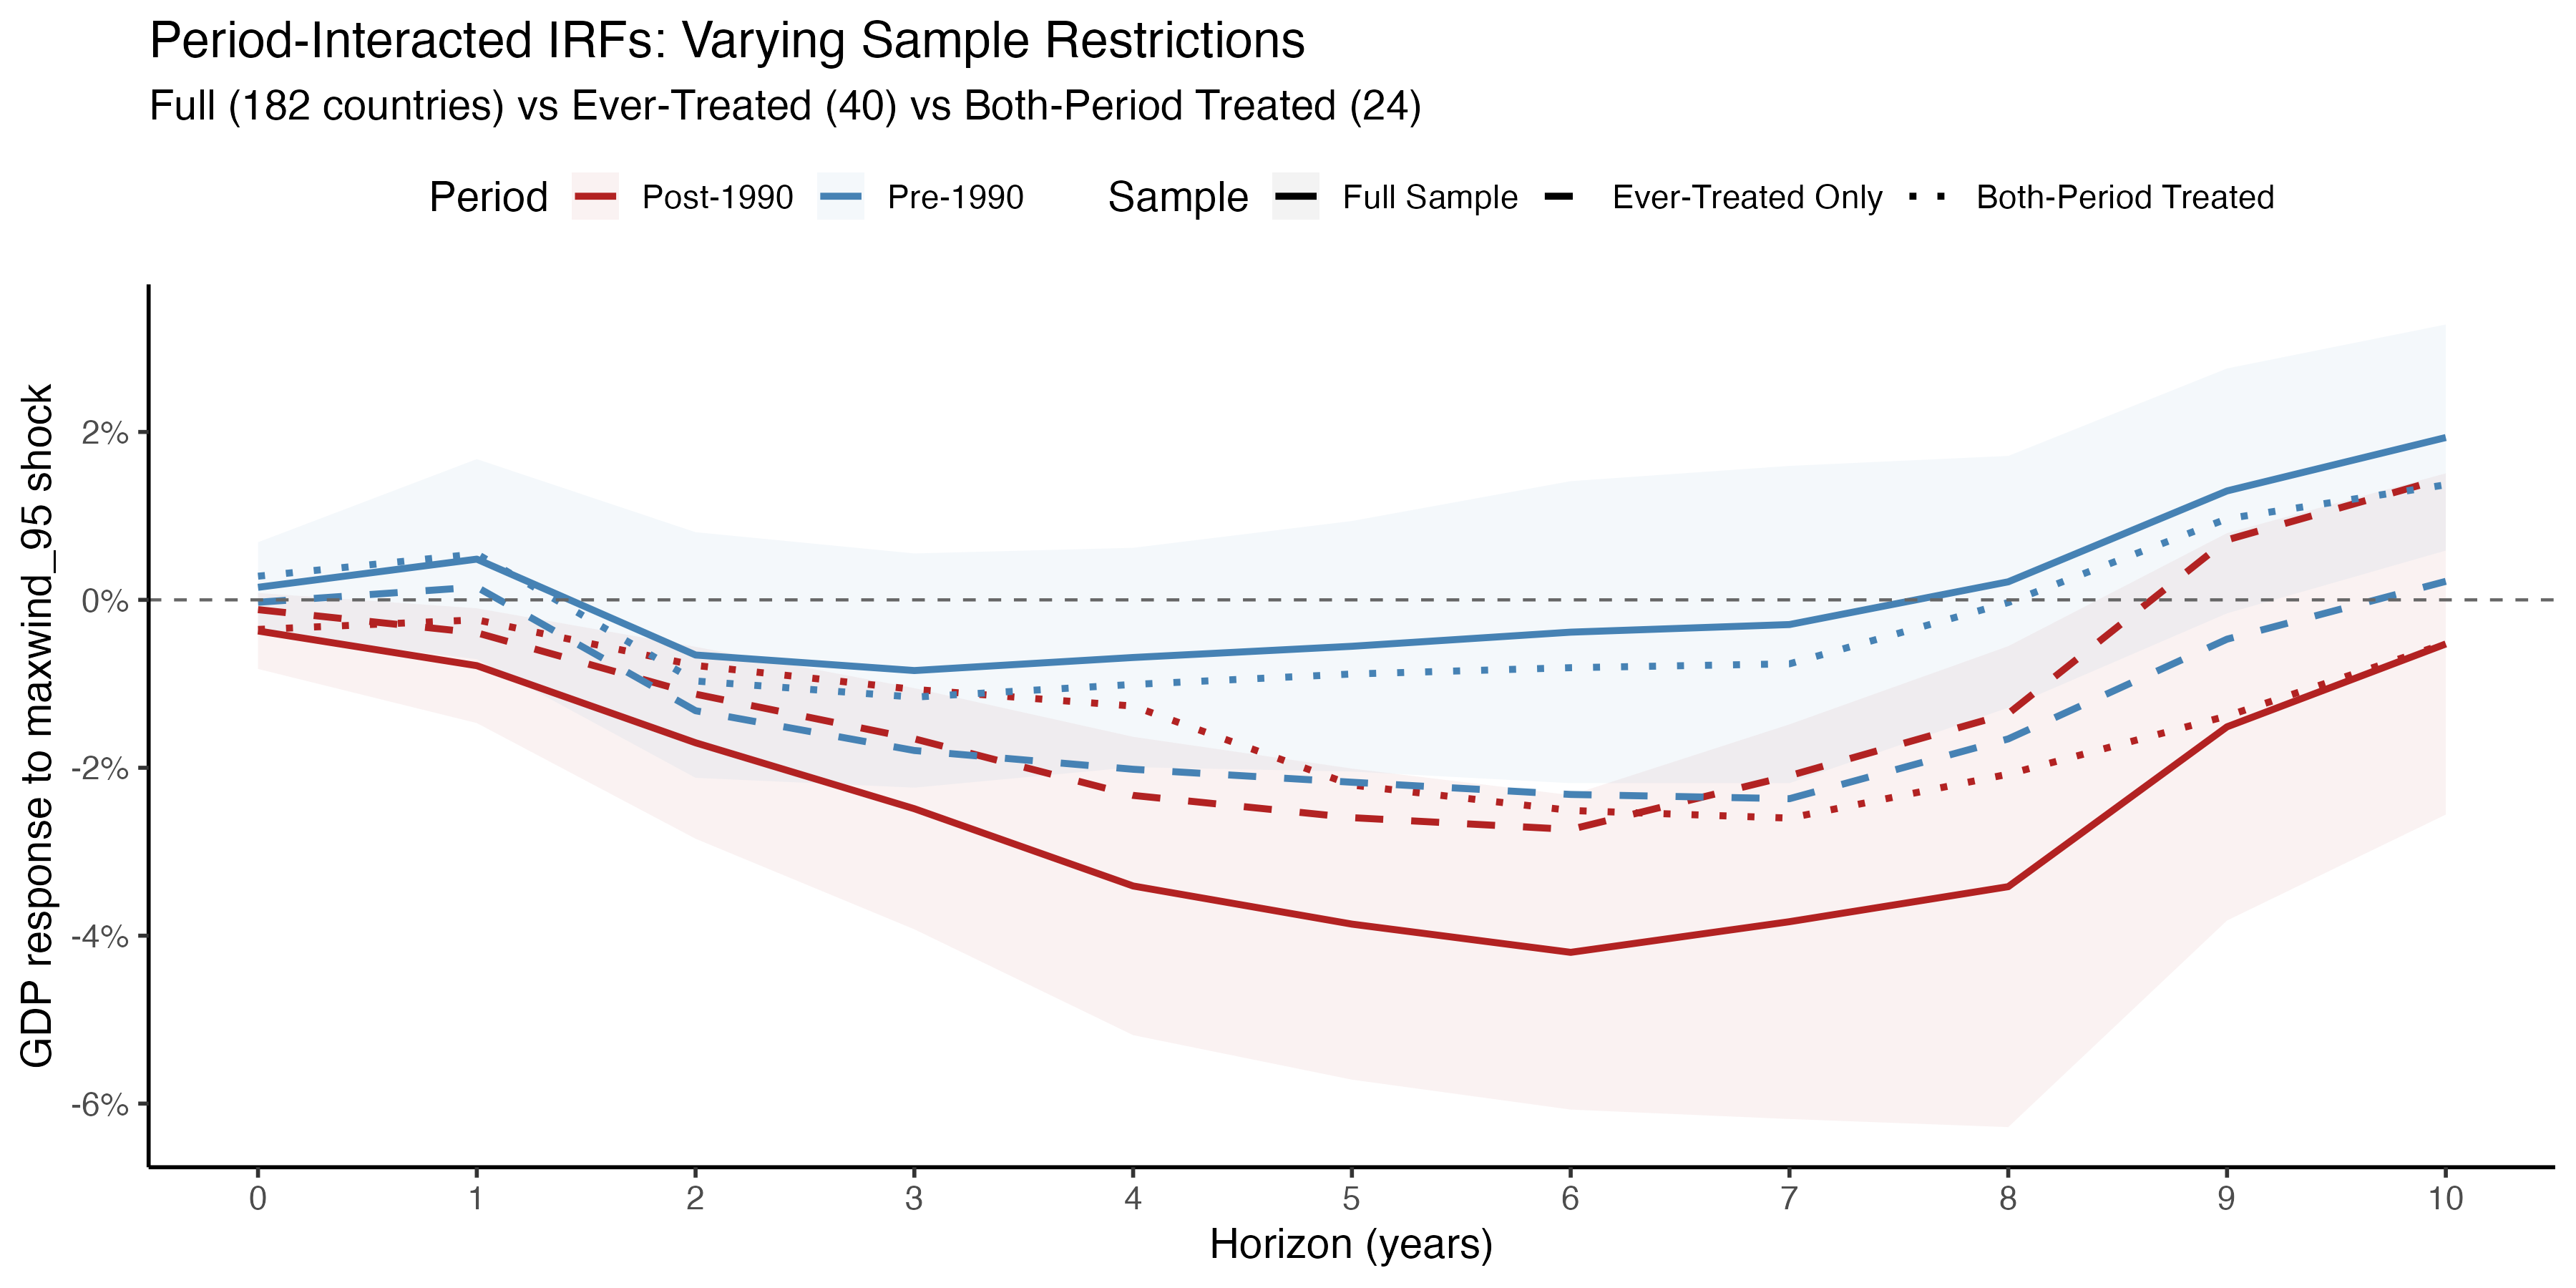
\includegraphics[width=\textwidth,height=0.68\textheight,keepaspectratio]{figures/irf_both_period_treated.png}

\smallskip
Full (182) vs.\ ever-treated (40) vs.\ both-period treated (24): the gap shrinks as the control group narrows.
\end{frame}

\begin{frame}{Year FE: Full vs.\ Ever-Treated Sample}
\centering
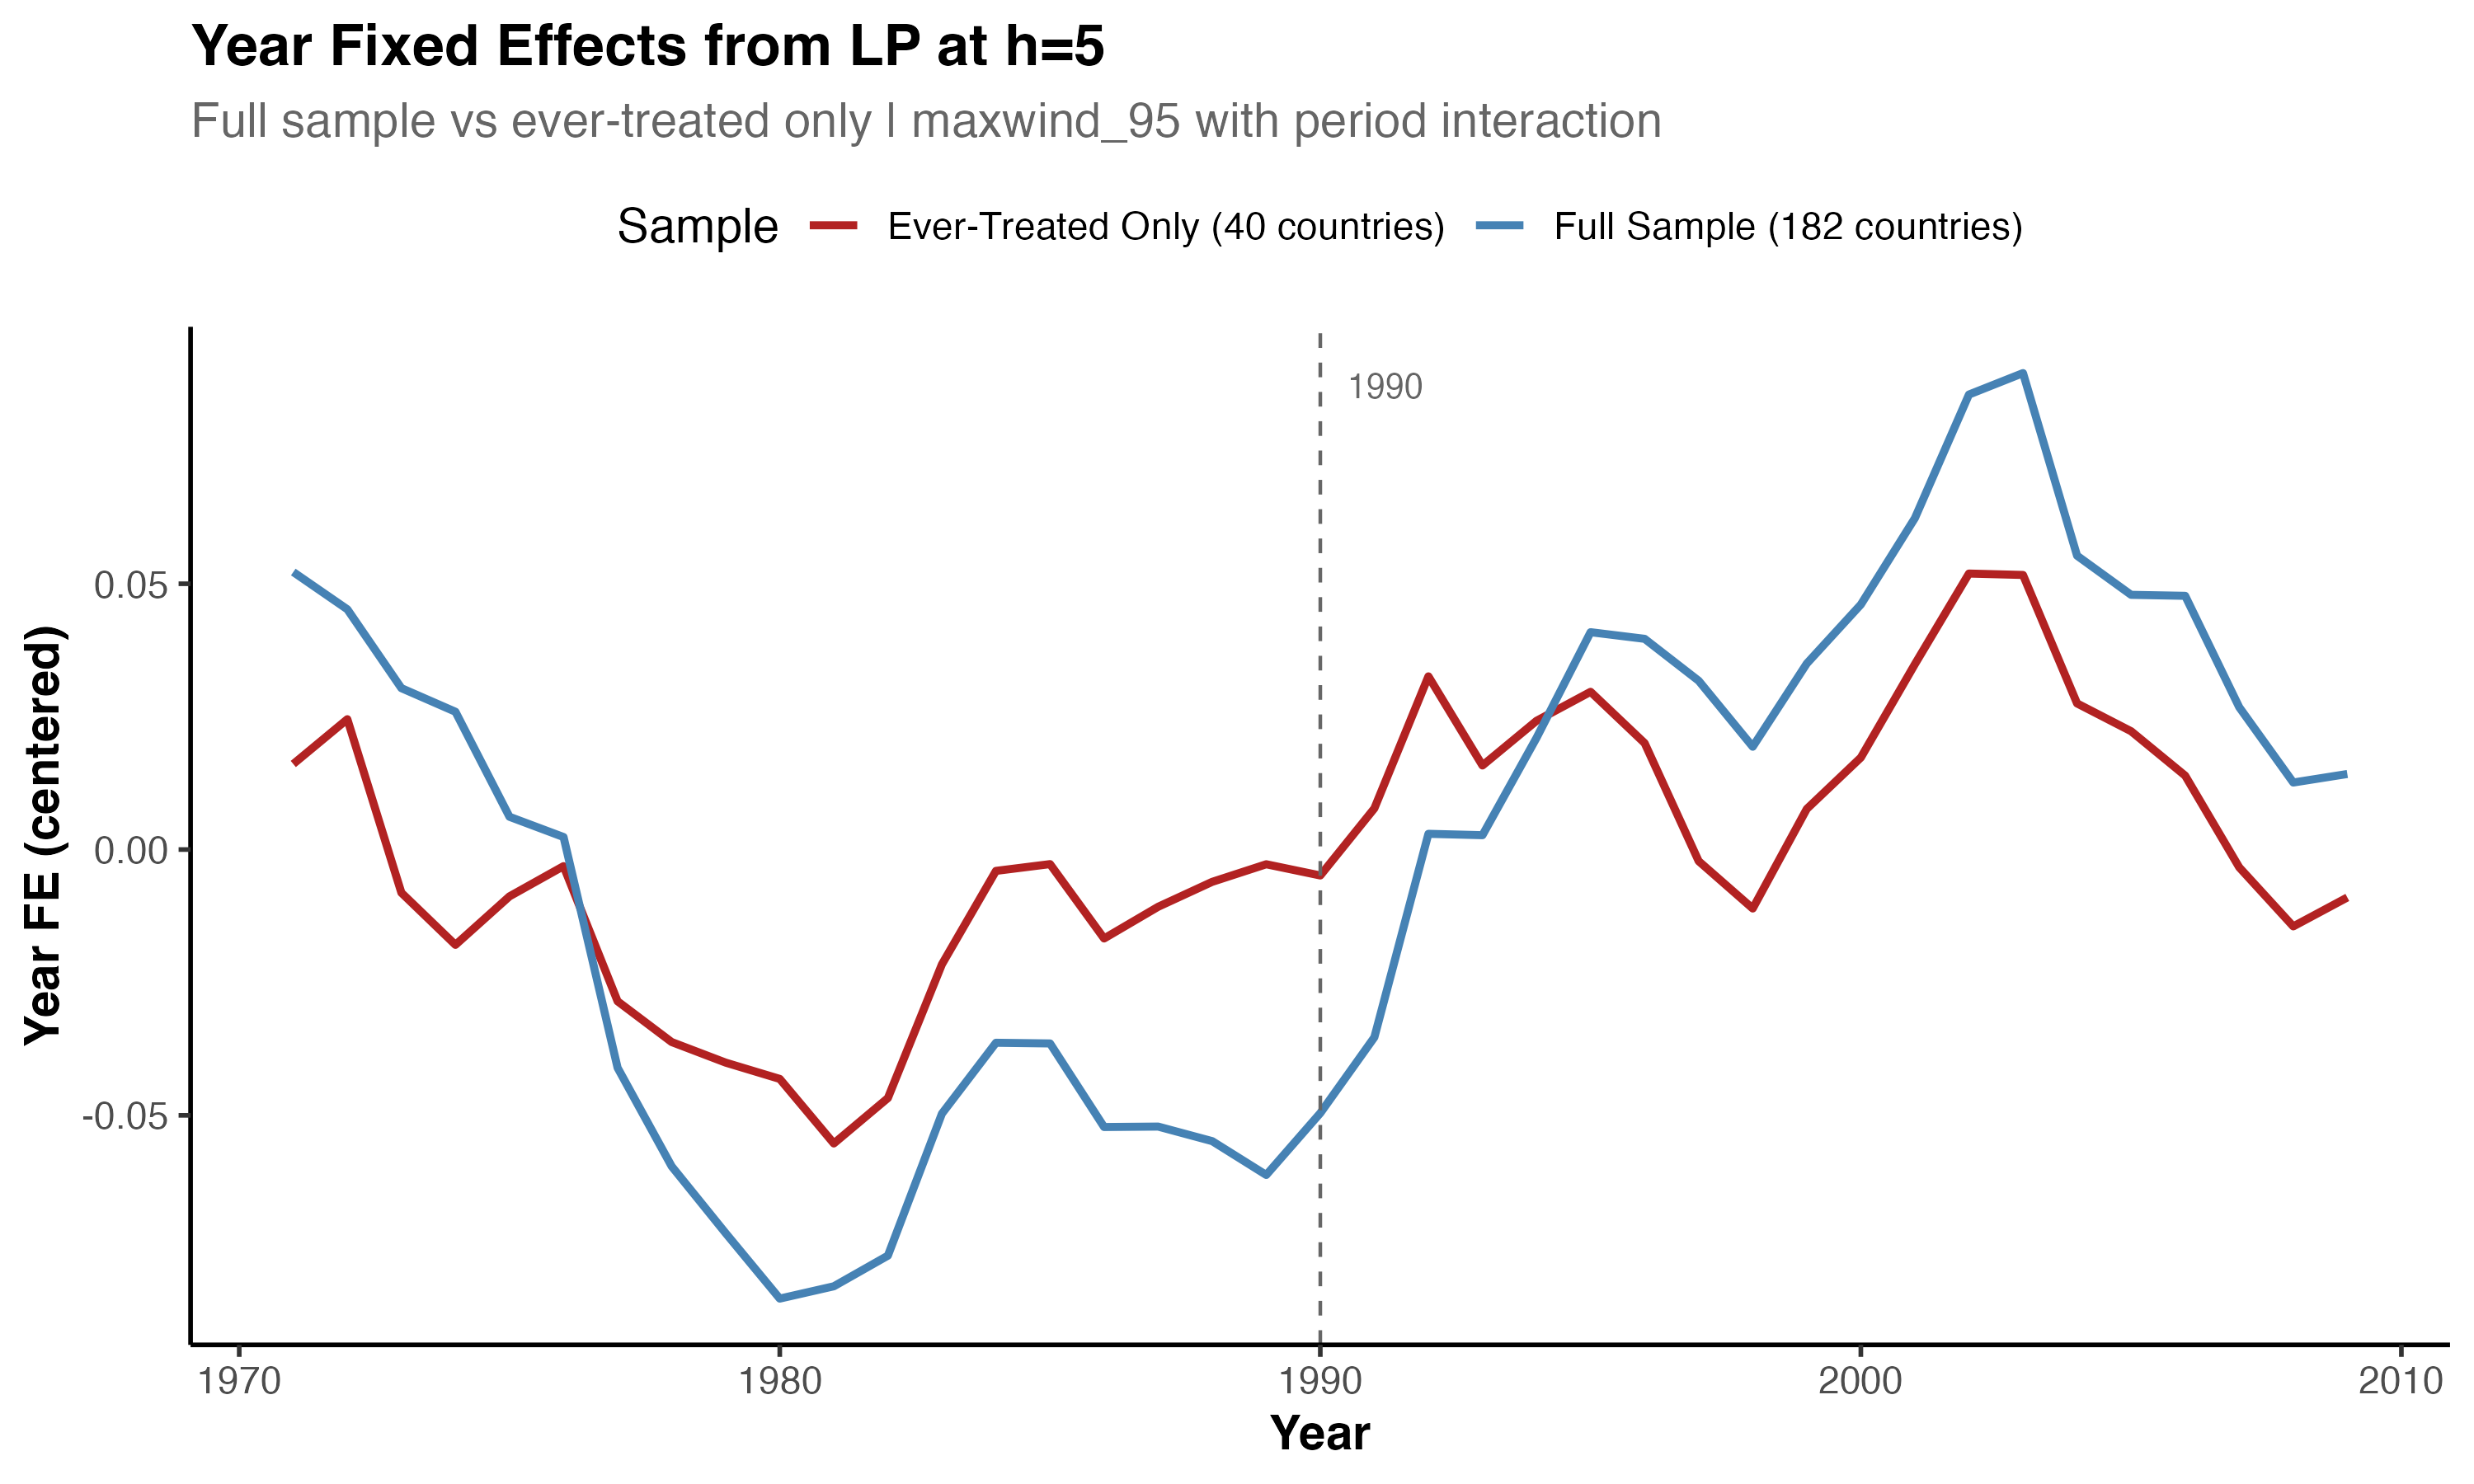
\includegraphics[width=0.85\textwidth,height=0.68\textheight,keepaspectratio]{figures/year_fe_decomposition.png}

\smallskip
Full-sample year FEs are lower pre-1990 and higher post-1990. Including never-treated countries inflates the post-1990 counterfactual.
\end{frame}

\begin{frame}{Which Never-Treated Countries Matter?}
\centering
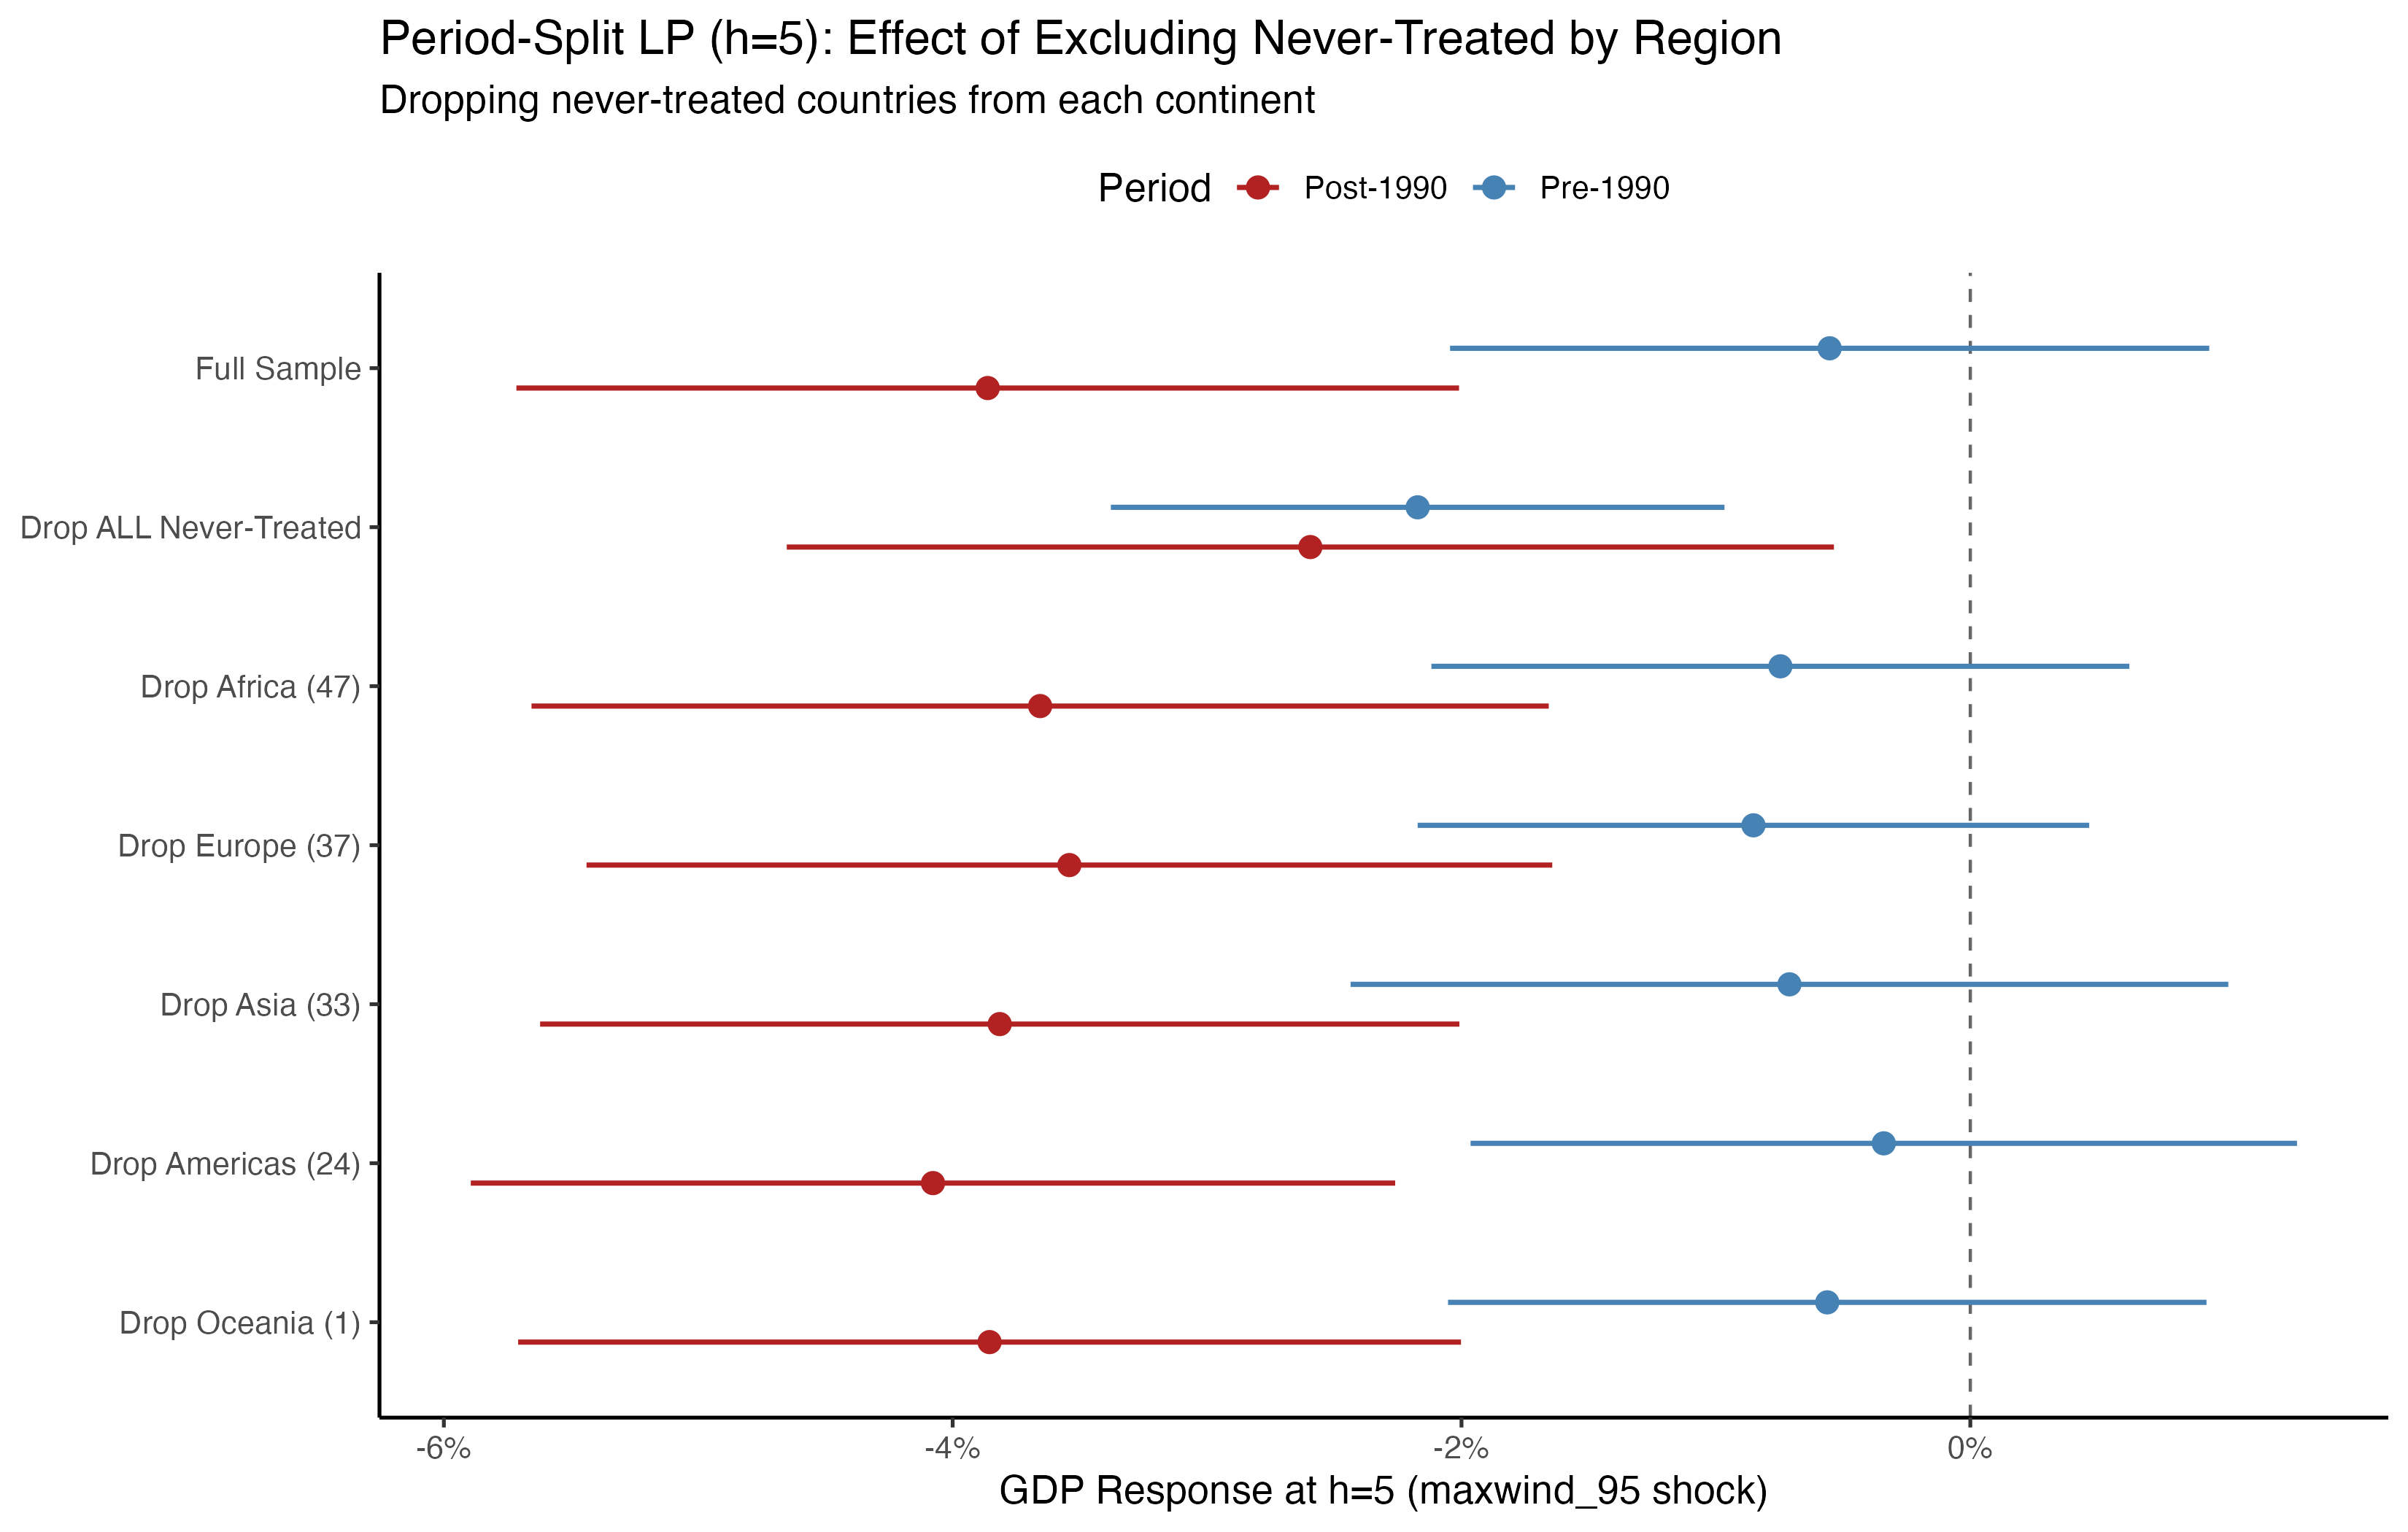
\includegraphics[width=0.85\textwidth,height=0.68\textheight,keepaspectratio]{figures/exclusion_by_region.png}

\smallskip
Europe has the largest effect. No single region accounts for the full attenuation.
\end{frame}

\begin{frame}{Solution: Region-Specific Year FE}
\centering
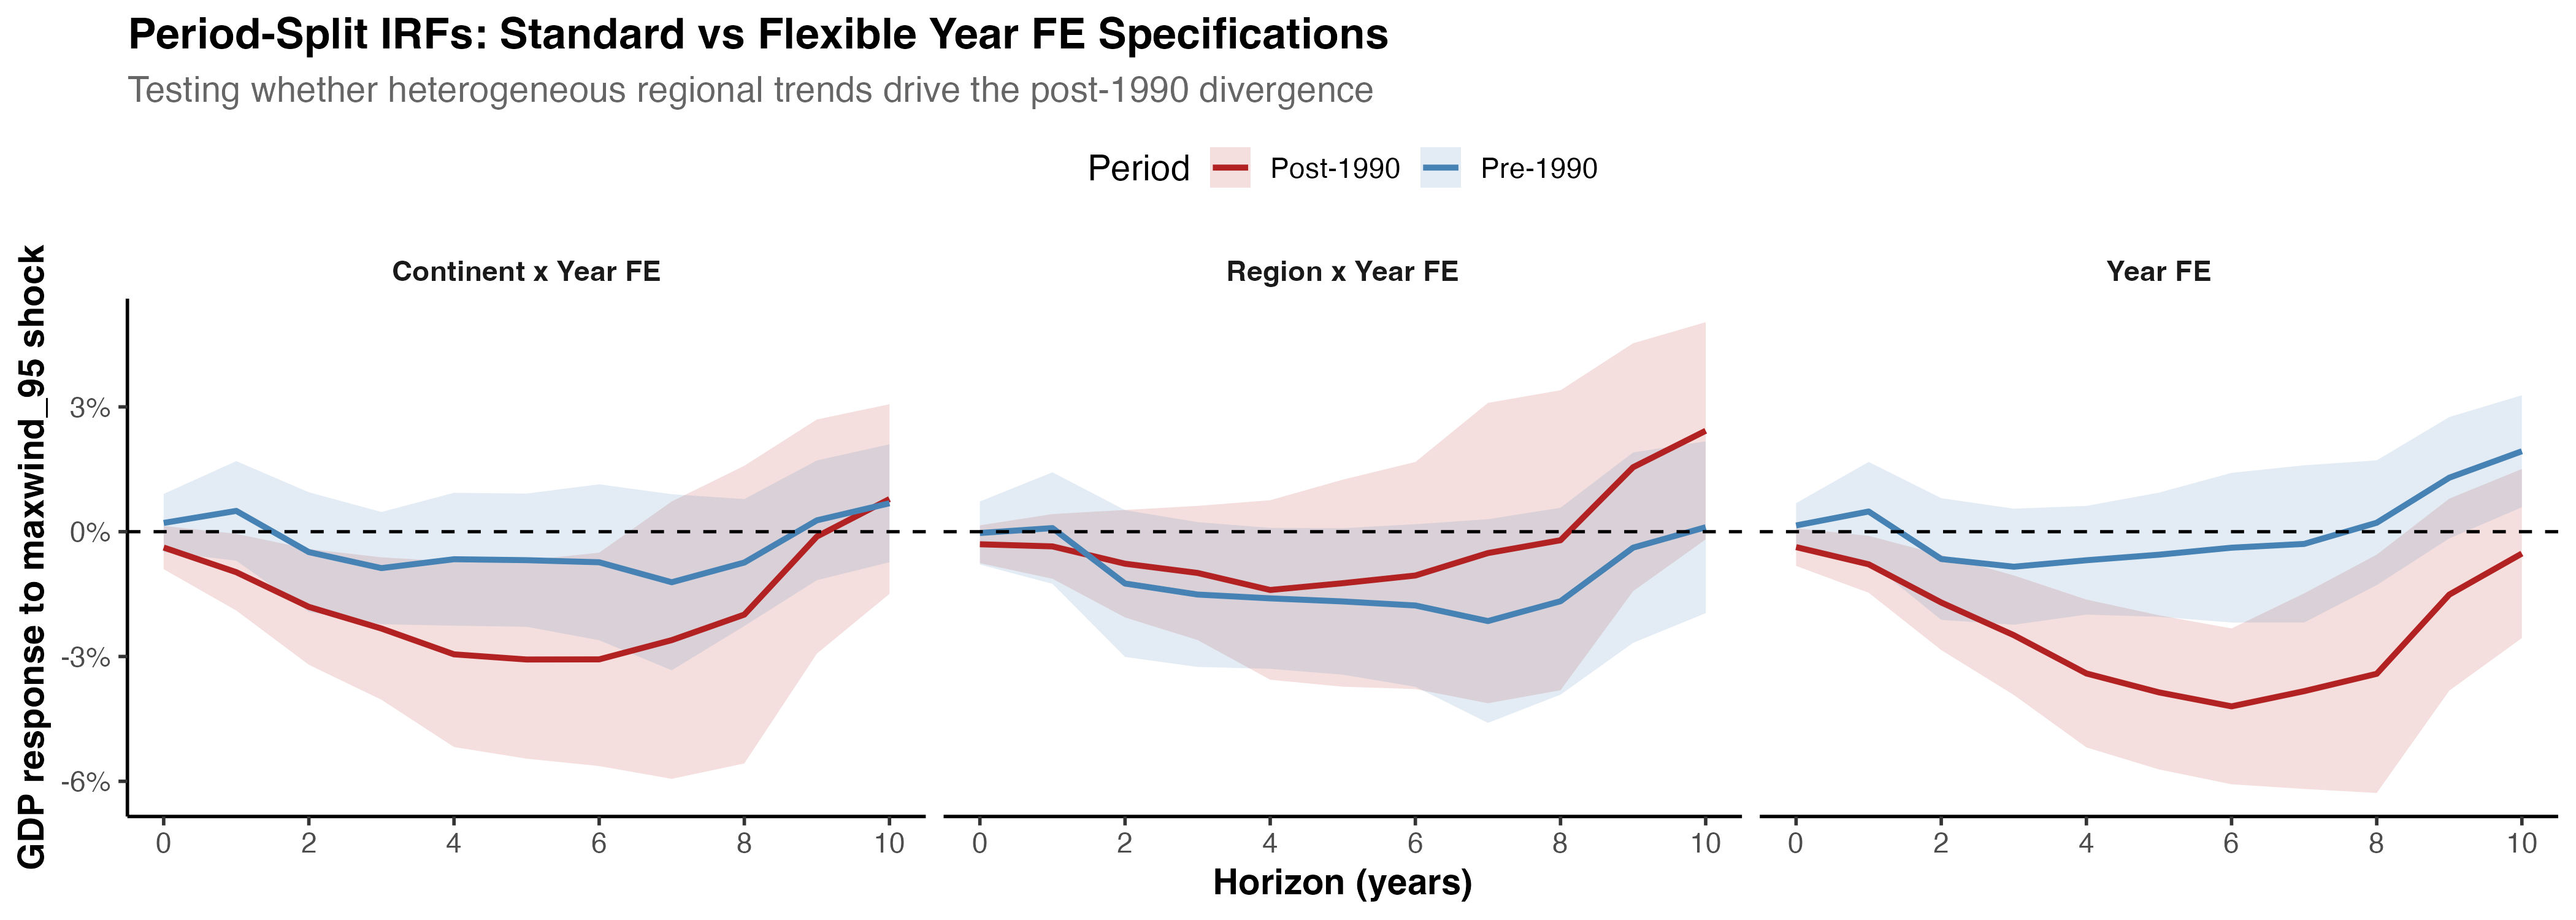
\includegraphics[width=\textwidth,height=0.62\textheight,keepaspectratio]{figures/irf_continent_year_fe.png}

\smallskip
\small
With continent$\times$year FE (5 groups: Africa, Americas, Asia, Europe, Oceania) the gap shrinks by 28\%. With region$\times$year FE (7 World Bank regions, e.g.\ East Asia \& Pacific, Sub-Saharan Africa) the divergence \textbf{vanishes entirely}.
\end{frame}

\begin{frame}{Placebo Test: Design}
If the control group is driving the post-1990 divergence, then \textbf{randomly assigning shocks to never-treated countries} should also produce a gap.

\medskip
\begin{enumerate}
  \item Take the 142 countries that never experience a real p95 cyclone shock
  \item Randomly assign placebo shocks matching the observed frequency and timing
  \item Estimate the period-interacted LP on this placebo-treated sample
  \item Record the post-1990 $-$ pre-1990 coefficient gap at $h = 5$
  \item Repeat 500 times to build a null distribution
\end{enumerate}

\medskip
\textbf{Test statistic}: the actual post$-$pre gap ($-0.033$) vs.\ the placebo distribution.

If $p$ is small, the real gap is unlikely under random assignment $\to$ the never-treated countries' GDP trends are systematically correlated with the counterfactual.
\end{frame}

\begin{frame}{Placebo Test: Results}
\centering
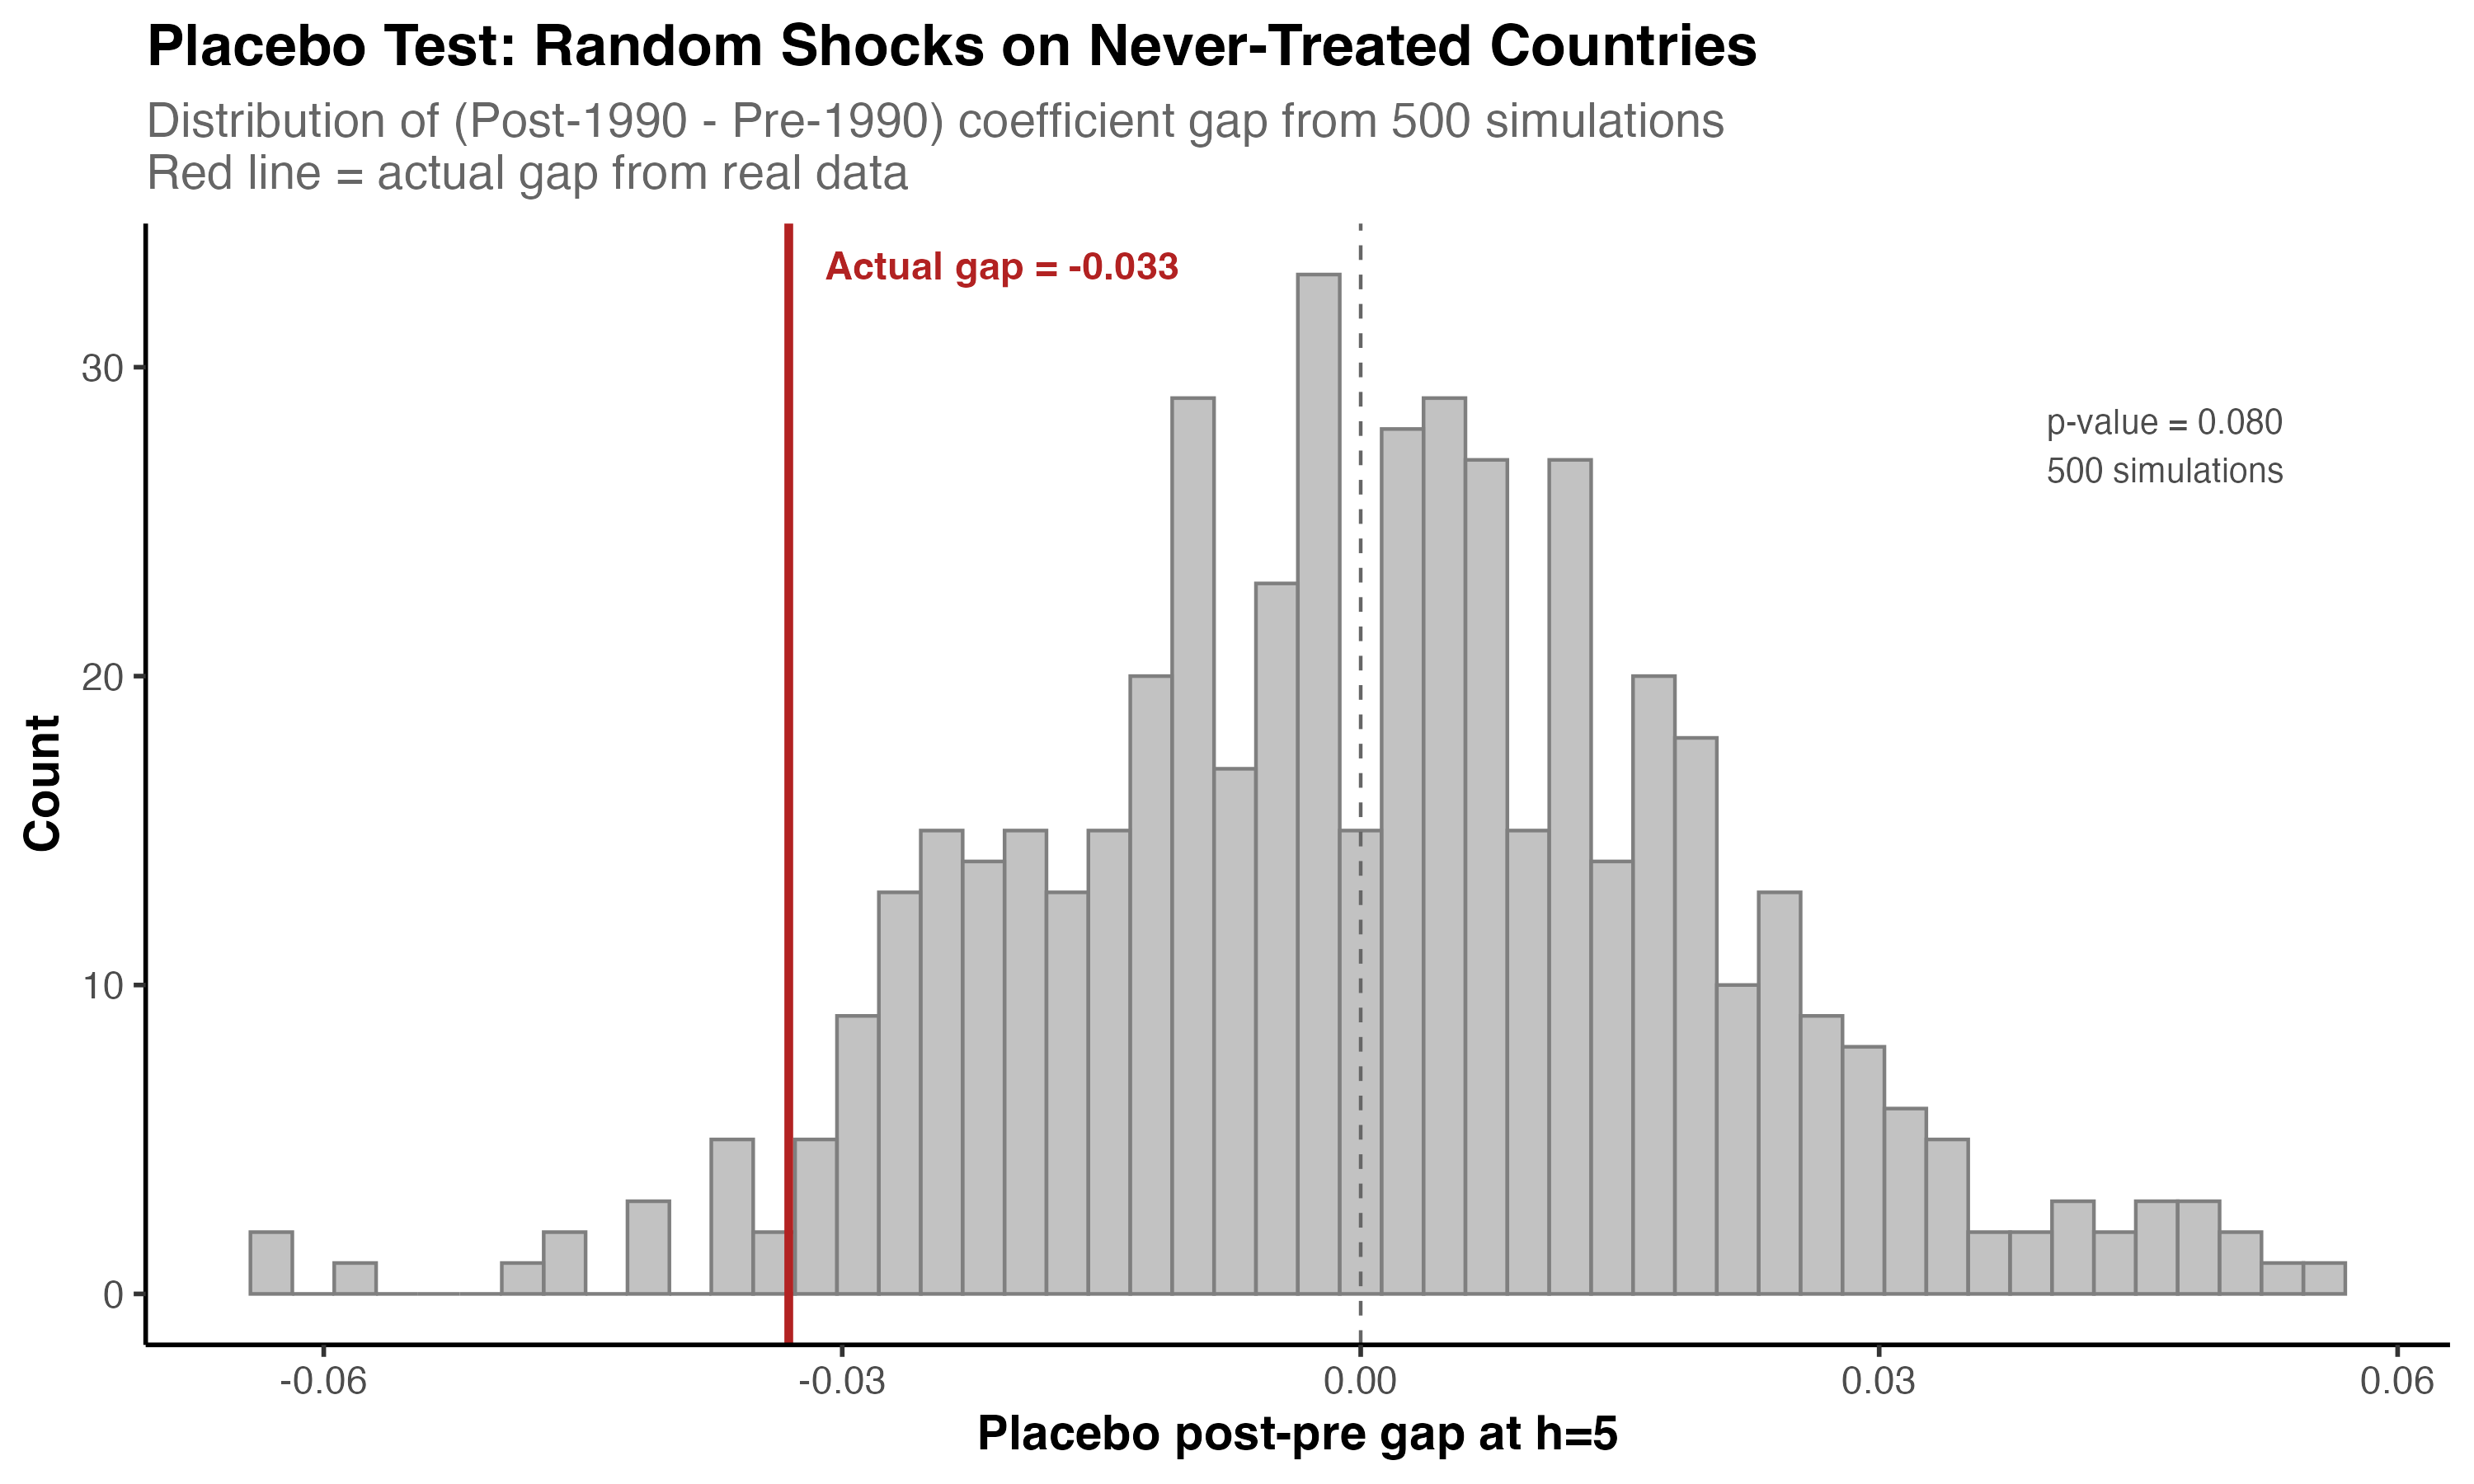
\includegraphics[width=0.85\textwidth,height=0.68\textheight,keepaspectratio]{figures/placebo_never_treated.png}

\smallskip
$p = 0.08$: the actual gap falls in the left tail. Consistent with control group composition contributing to the result.
\end{frame}

% ===============================================================
\section{Robustness}
% ===============================================================

{\hideframenumber
\begin{frame}
\sectionpage
\end{frame}
\showframenumber}

\begin{frame}{Leave-One-Year-Out}
\centering
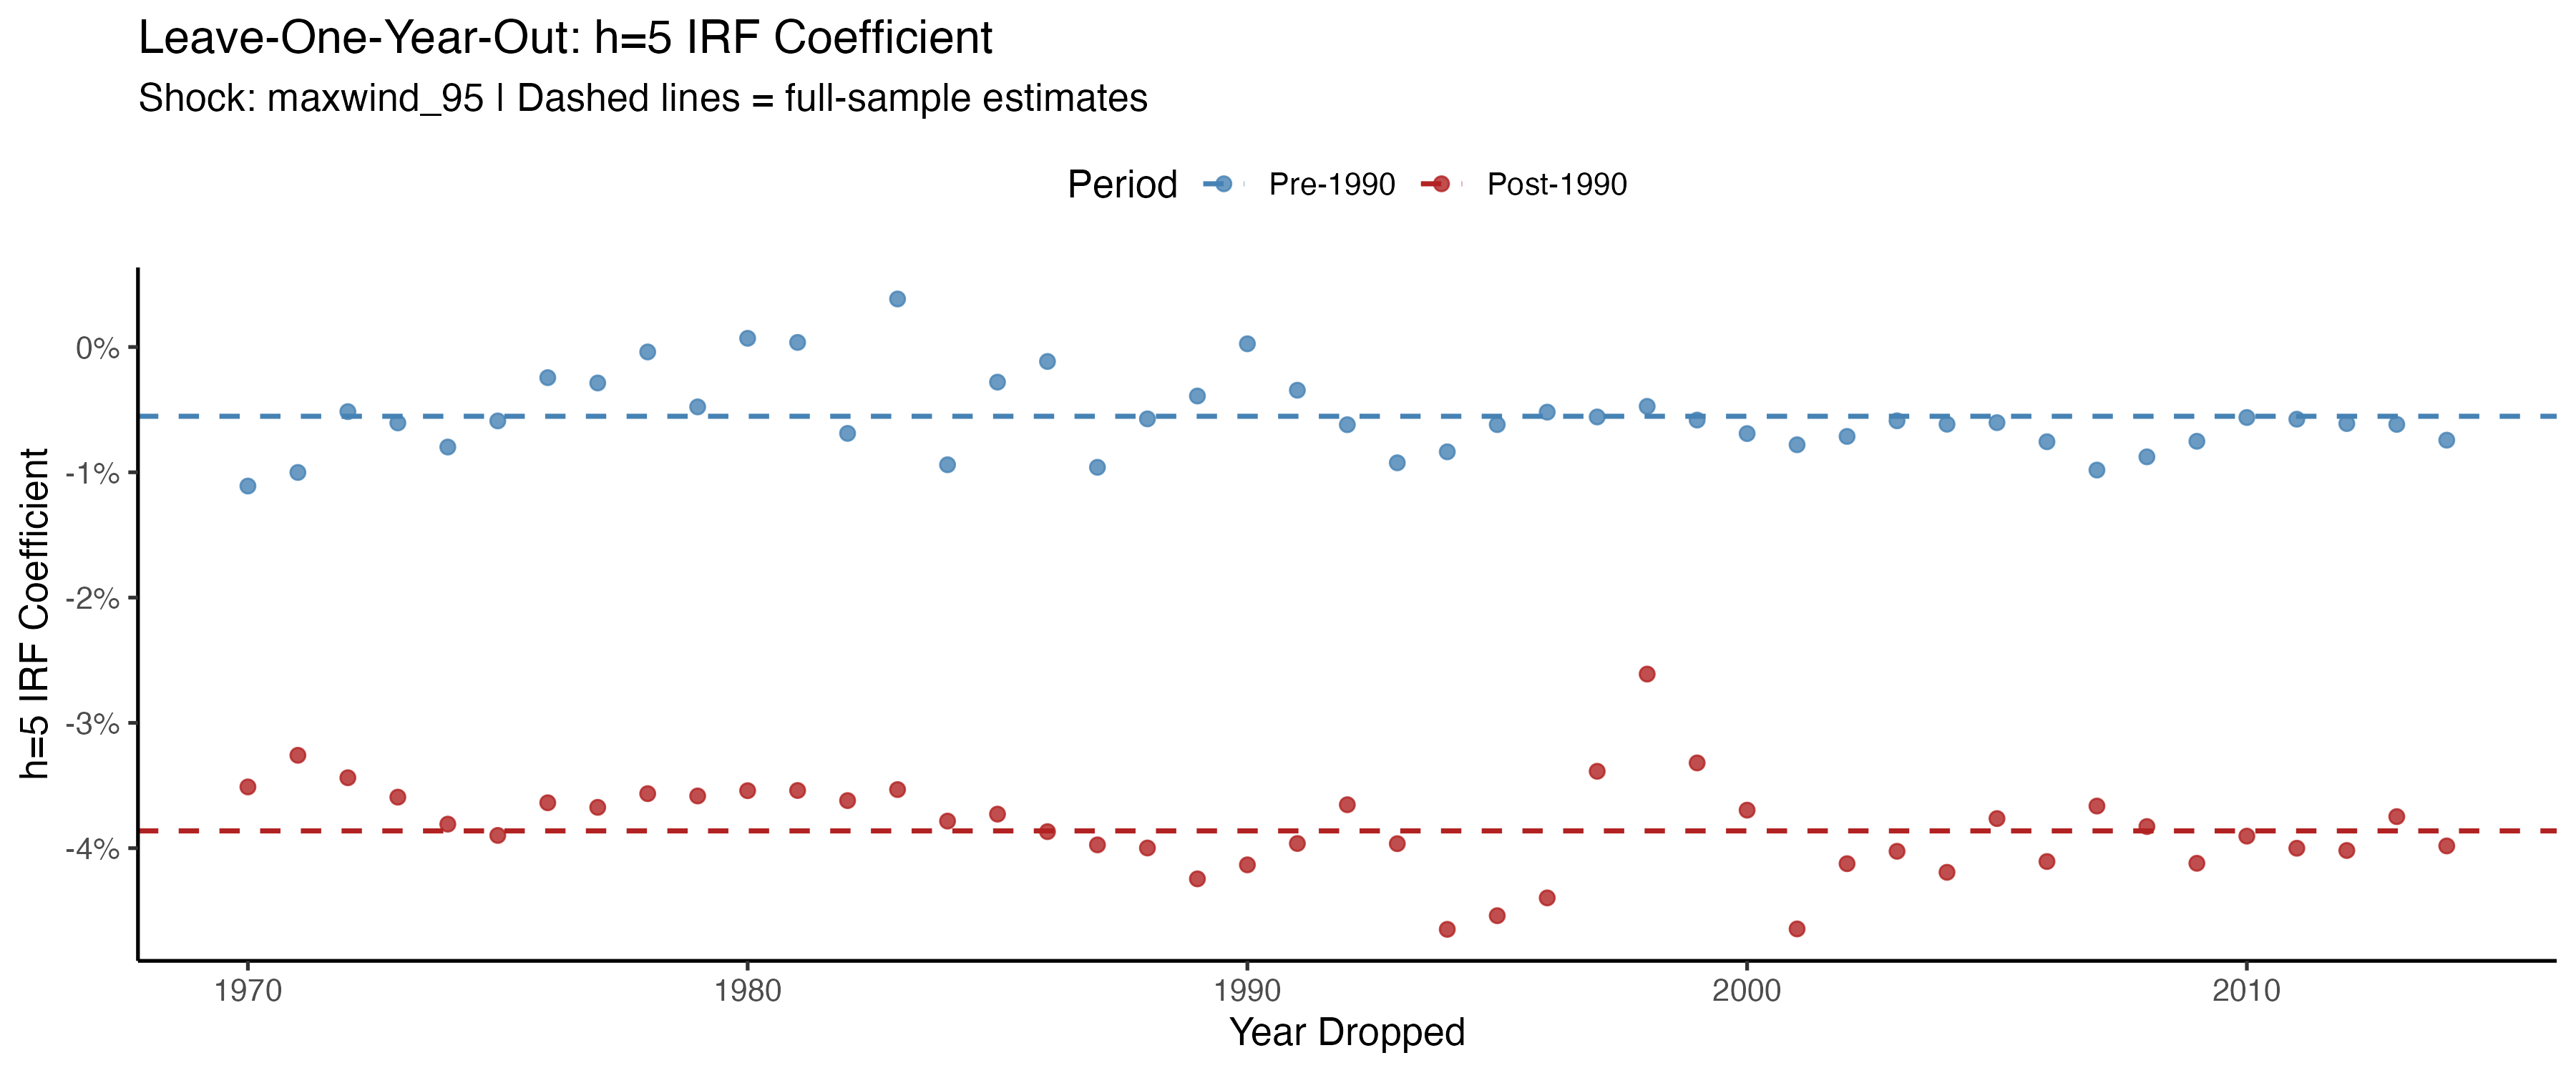
\includegraphics[width=\textwidth,height=0.72\textheight,keepaspectratio]{figures/loo_year_influence.png}

\smallskip
No single year flips the result. 1998 (Hurricane Mitch) is most influential.
\end{frame}

\begin{frame}{Leave-One-Country-Out}
\centering
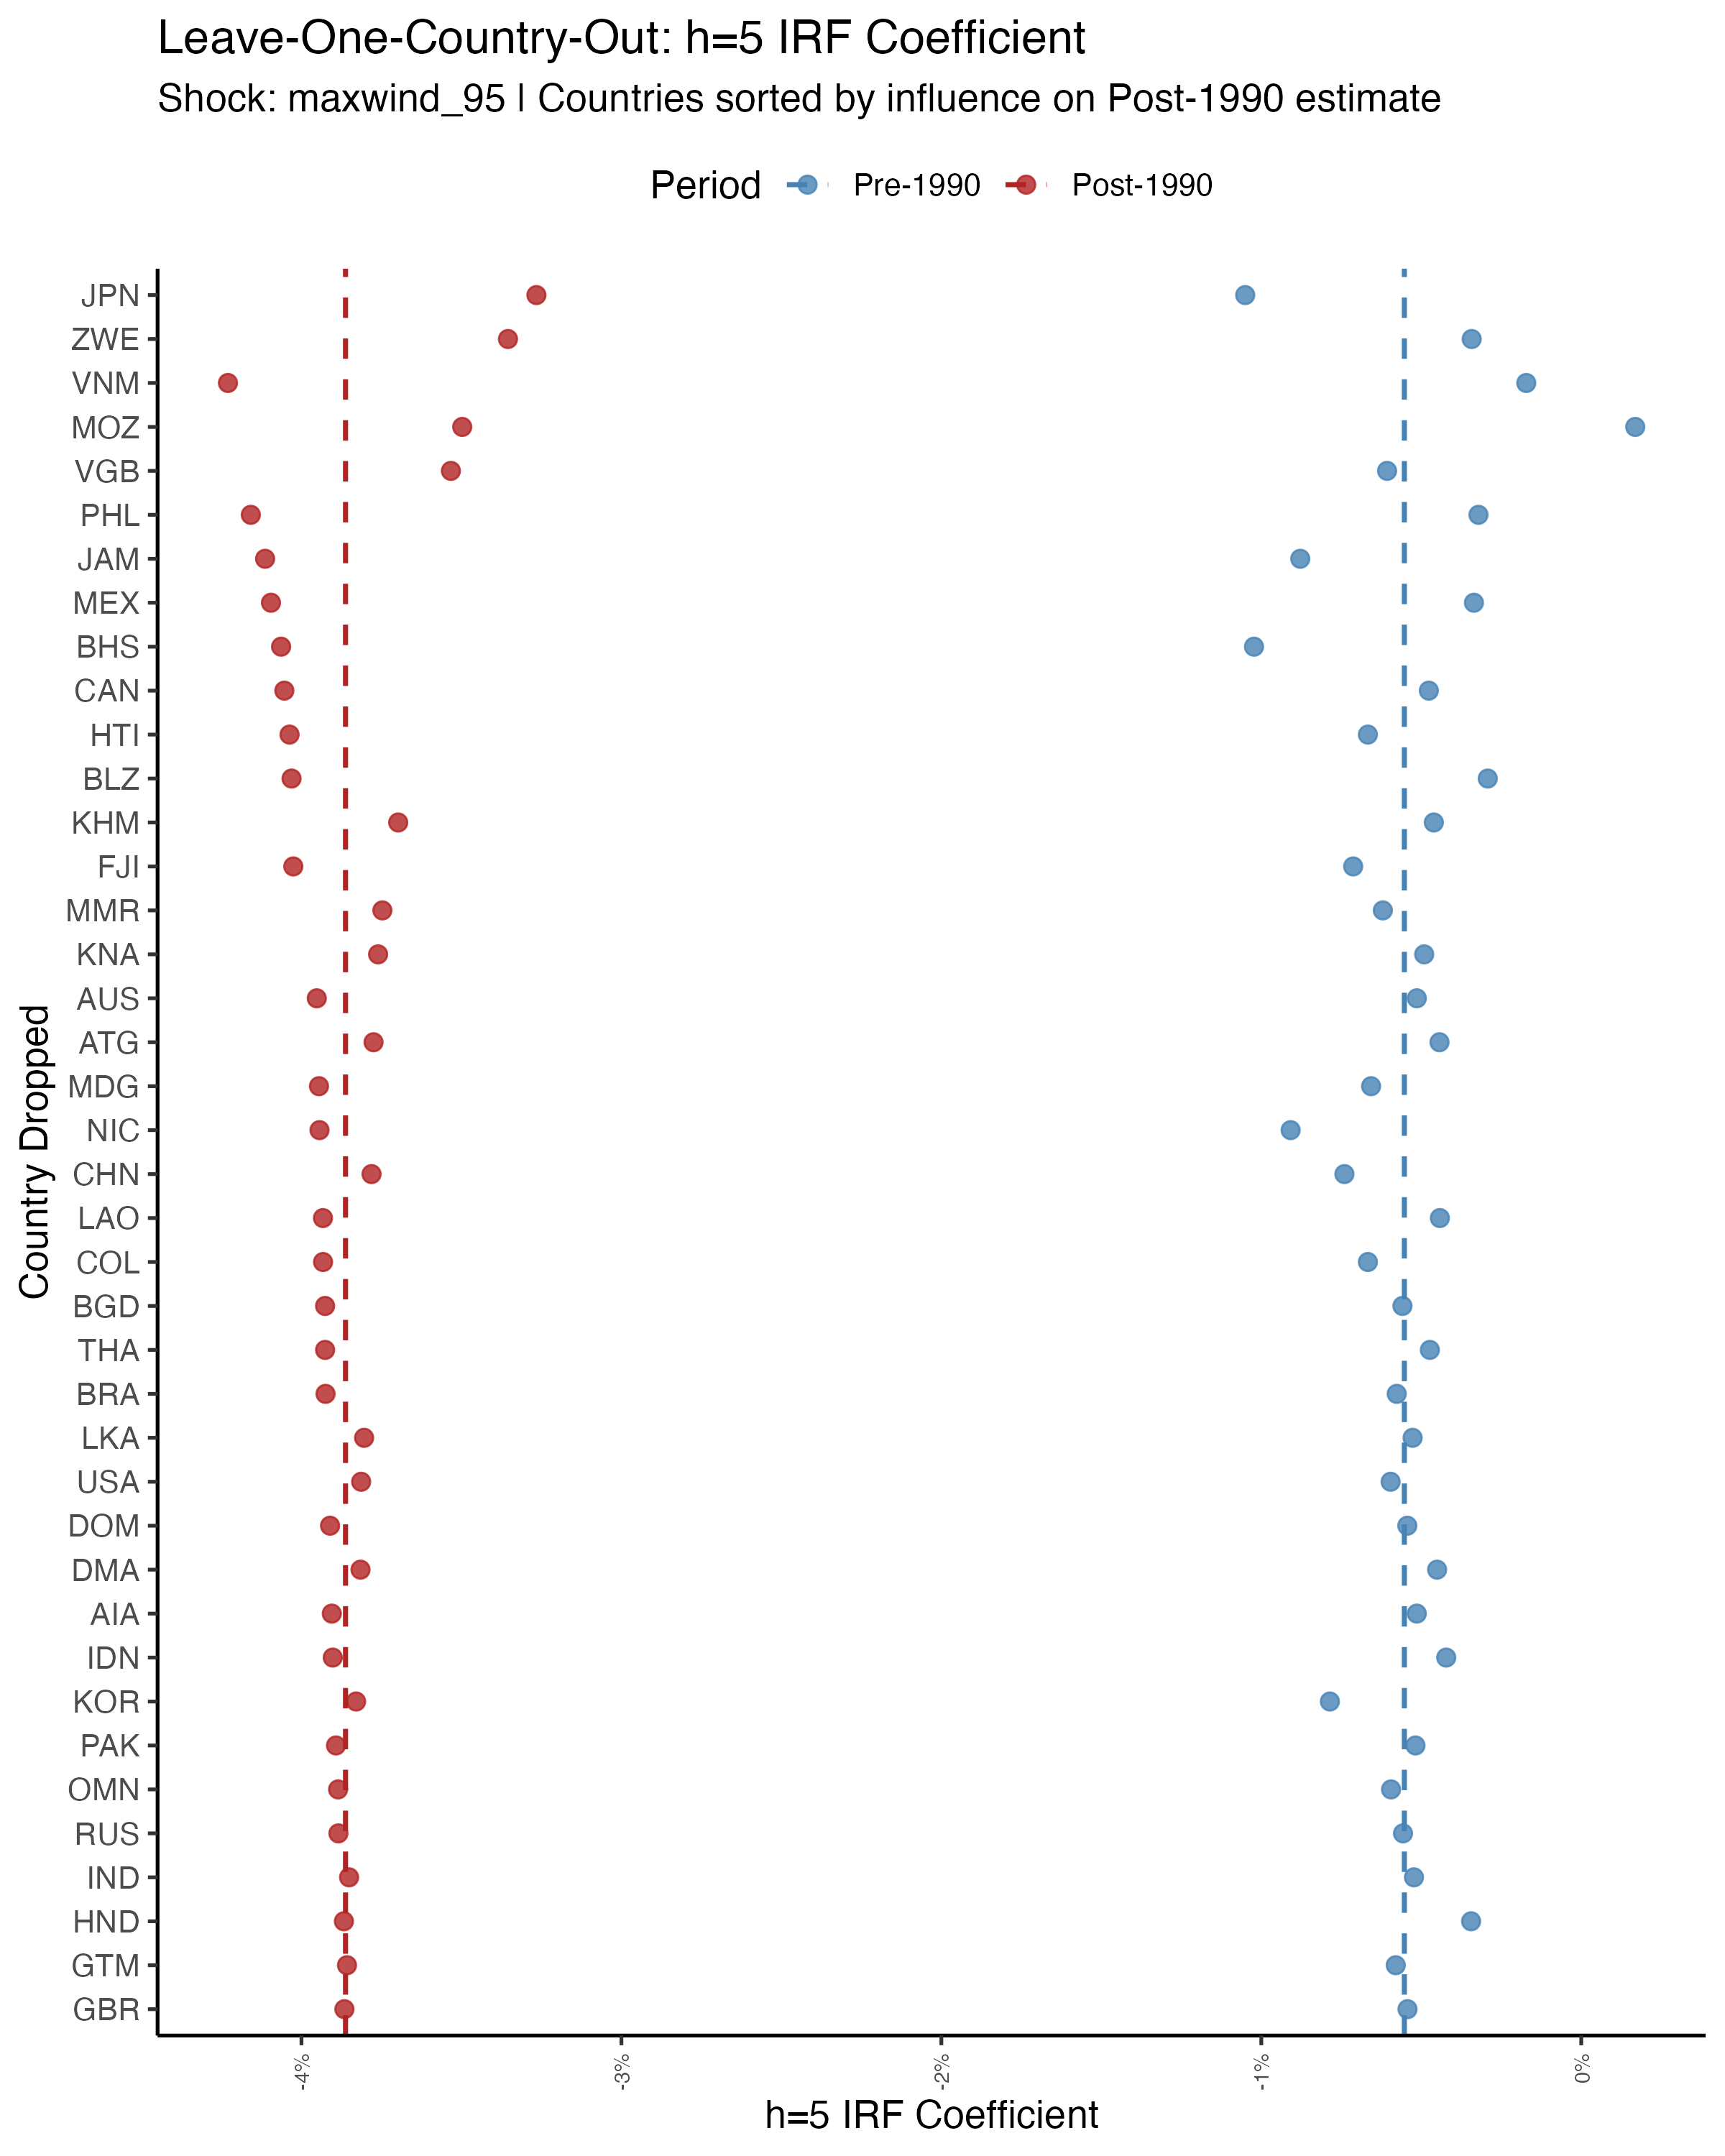
\includegraphics[width=\textwidth,height=0.72\textheight,keepaspectratio]{figures/loo_country_influence.png}

\smallskip
Coefficient ranges from $-3.3\%$ to $-4.2\%$. Japan is most influential but its removal does not eliminate the effect.
\end{frame}

\begin{frame}{Leave-One-Out: Top 5 Exposed Countries}
\centering
\begin{columns}[T]
\column{0.48\textwidth}
\centering
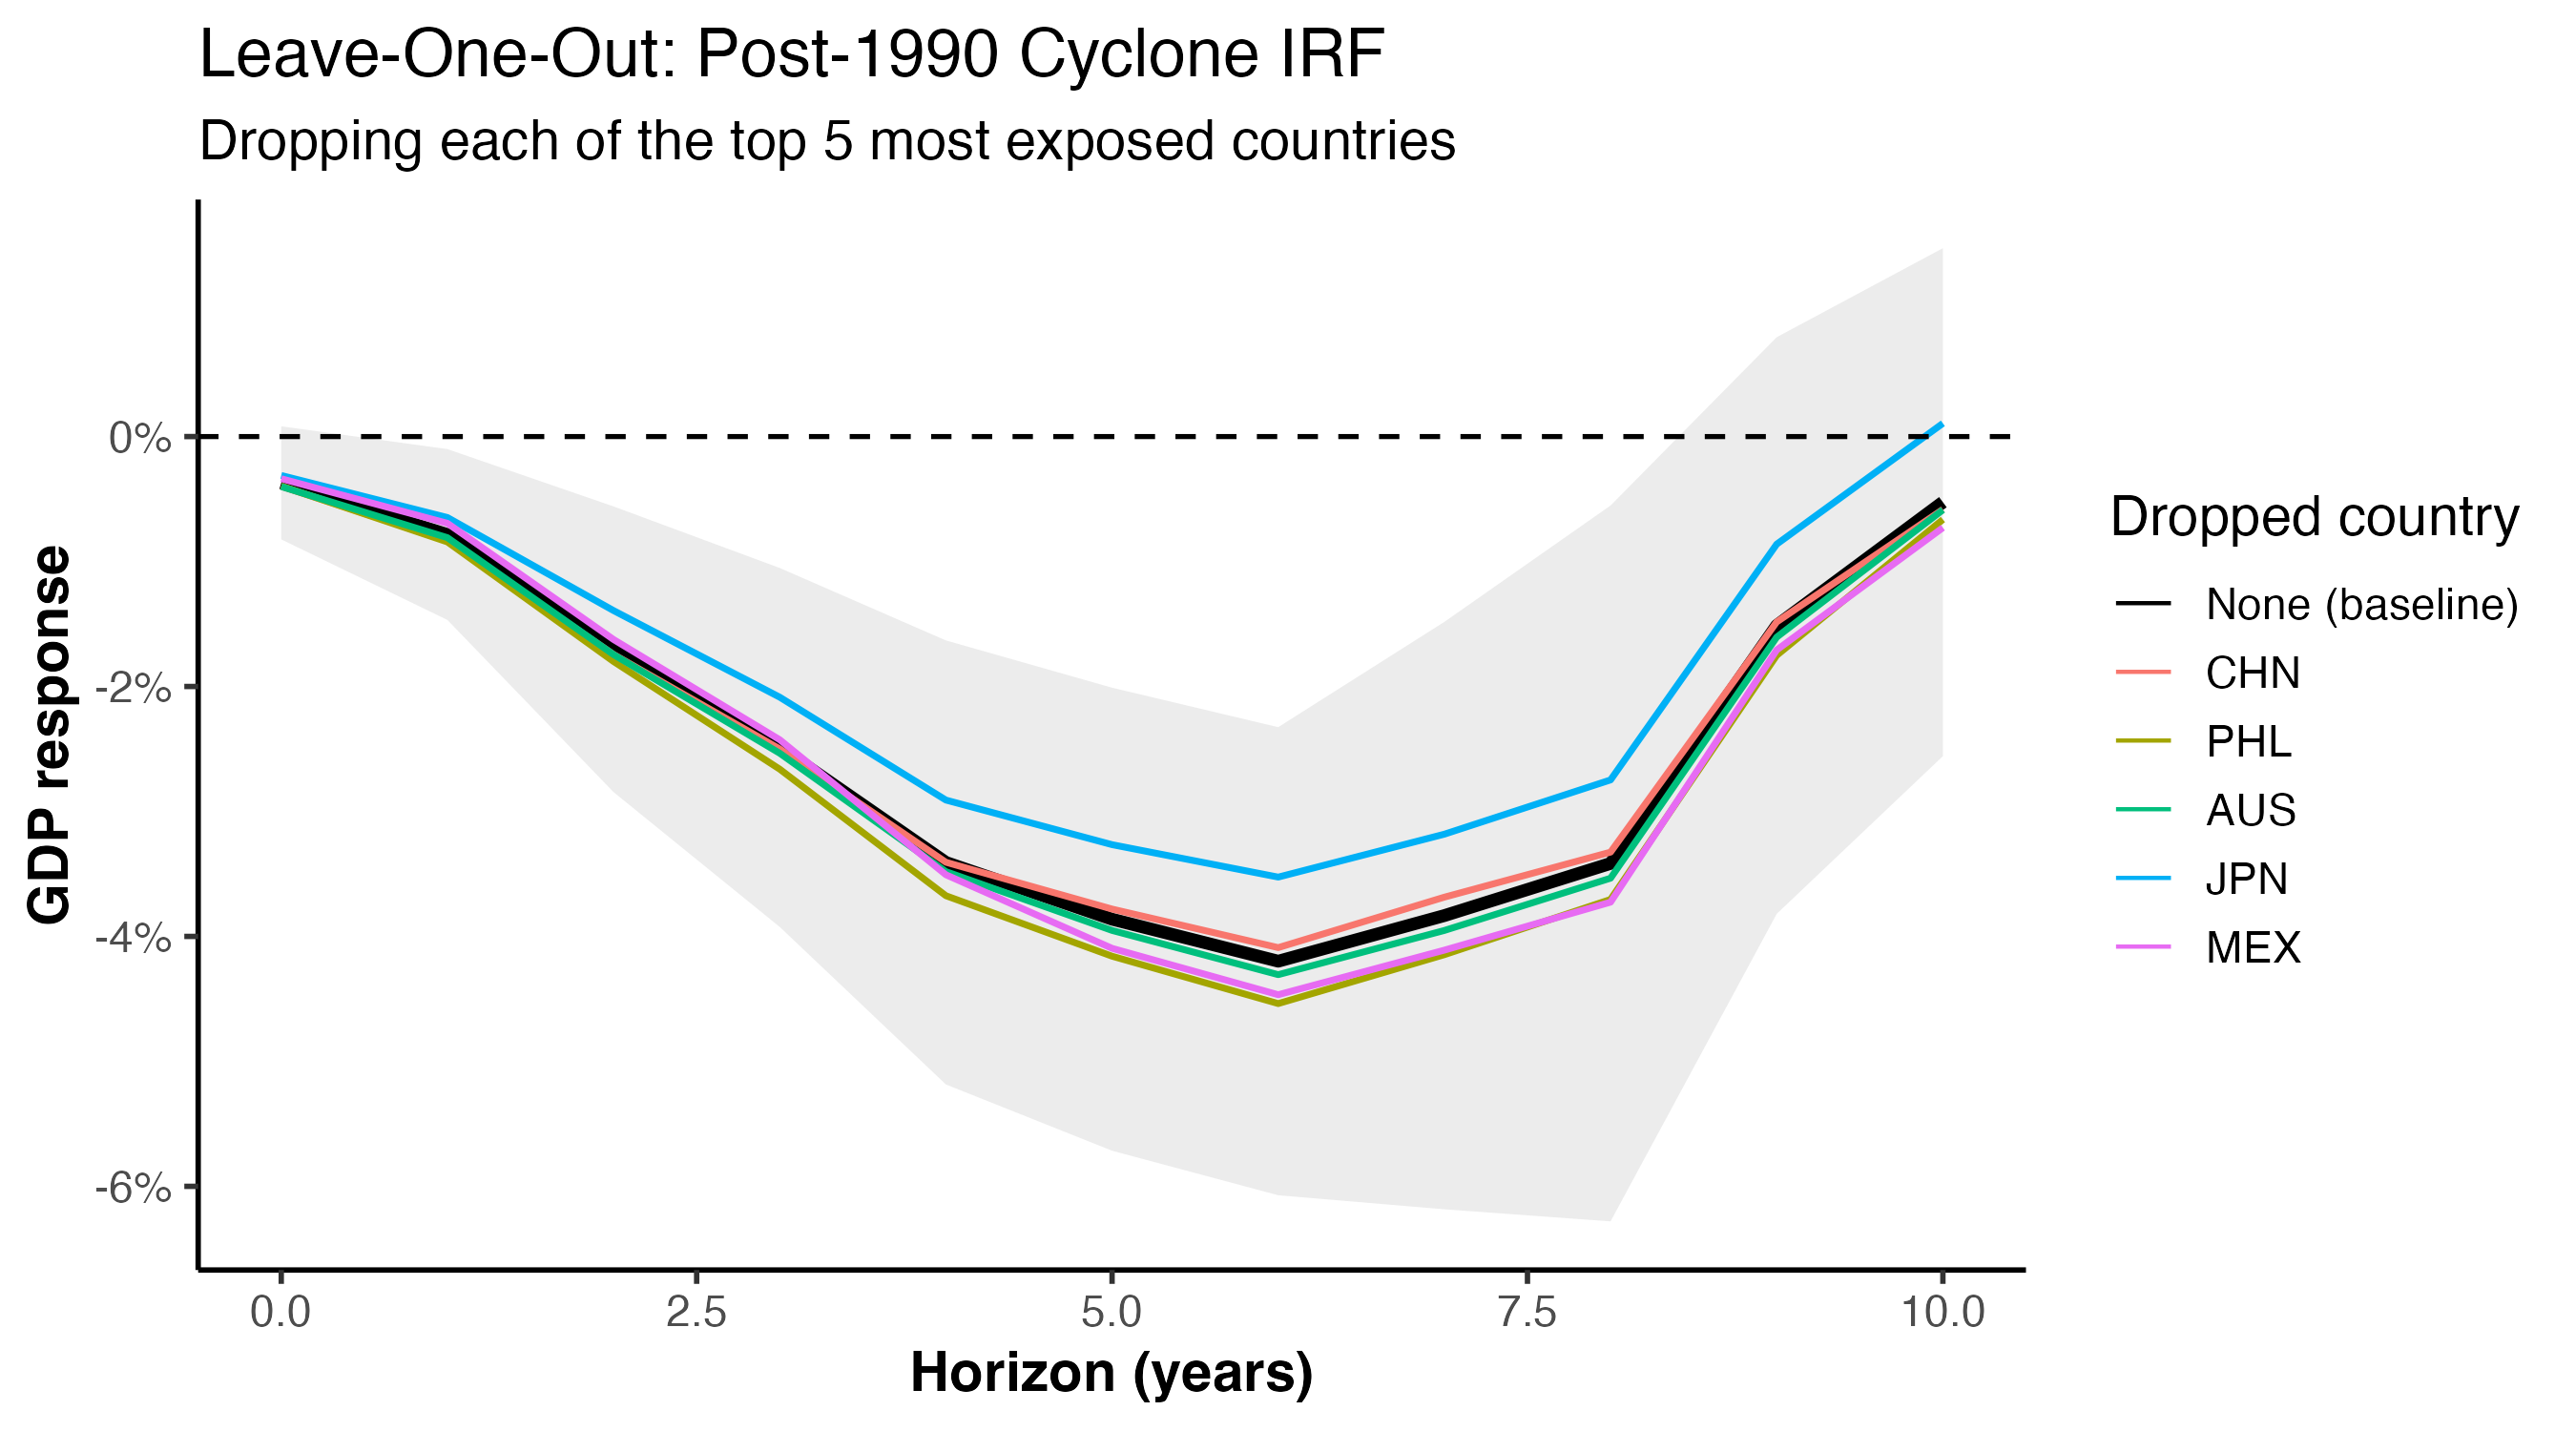
\includegraphics[width=\textwidth,height=0.65\textheight,keepaspectratio]{figures/vulnerability_loo_post1990.png}

\smallskip
{\small Post-1990 only}

\column{0.48\textwidth}
\centering
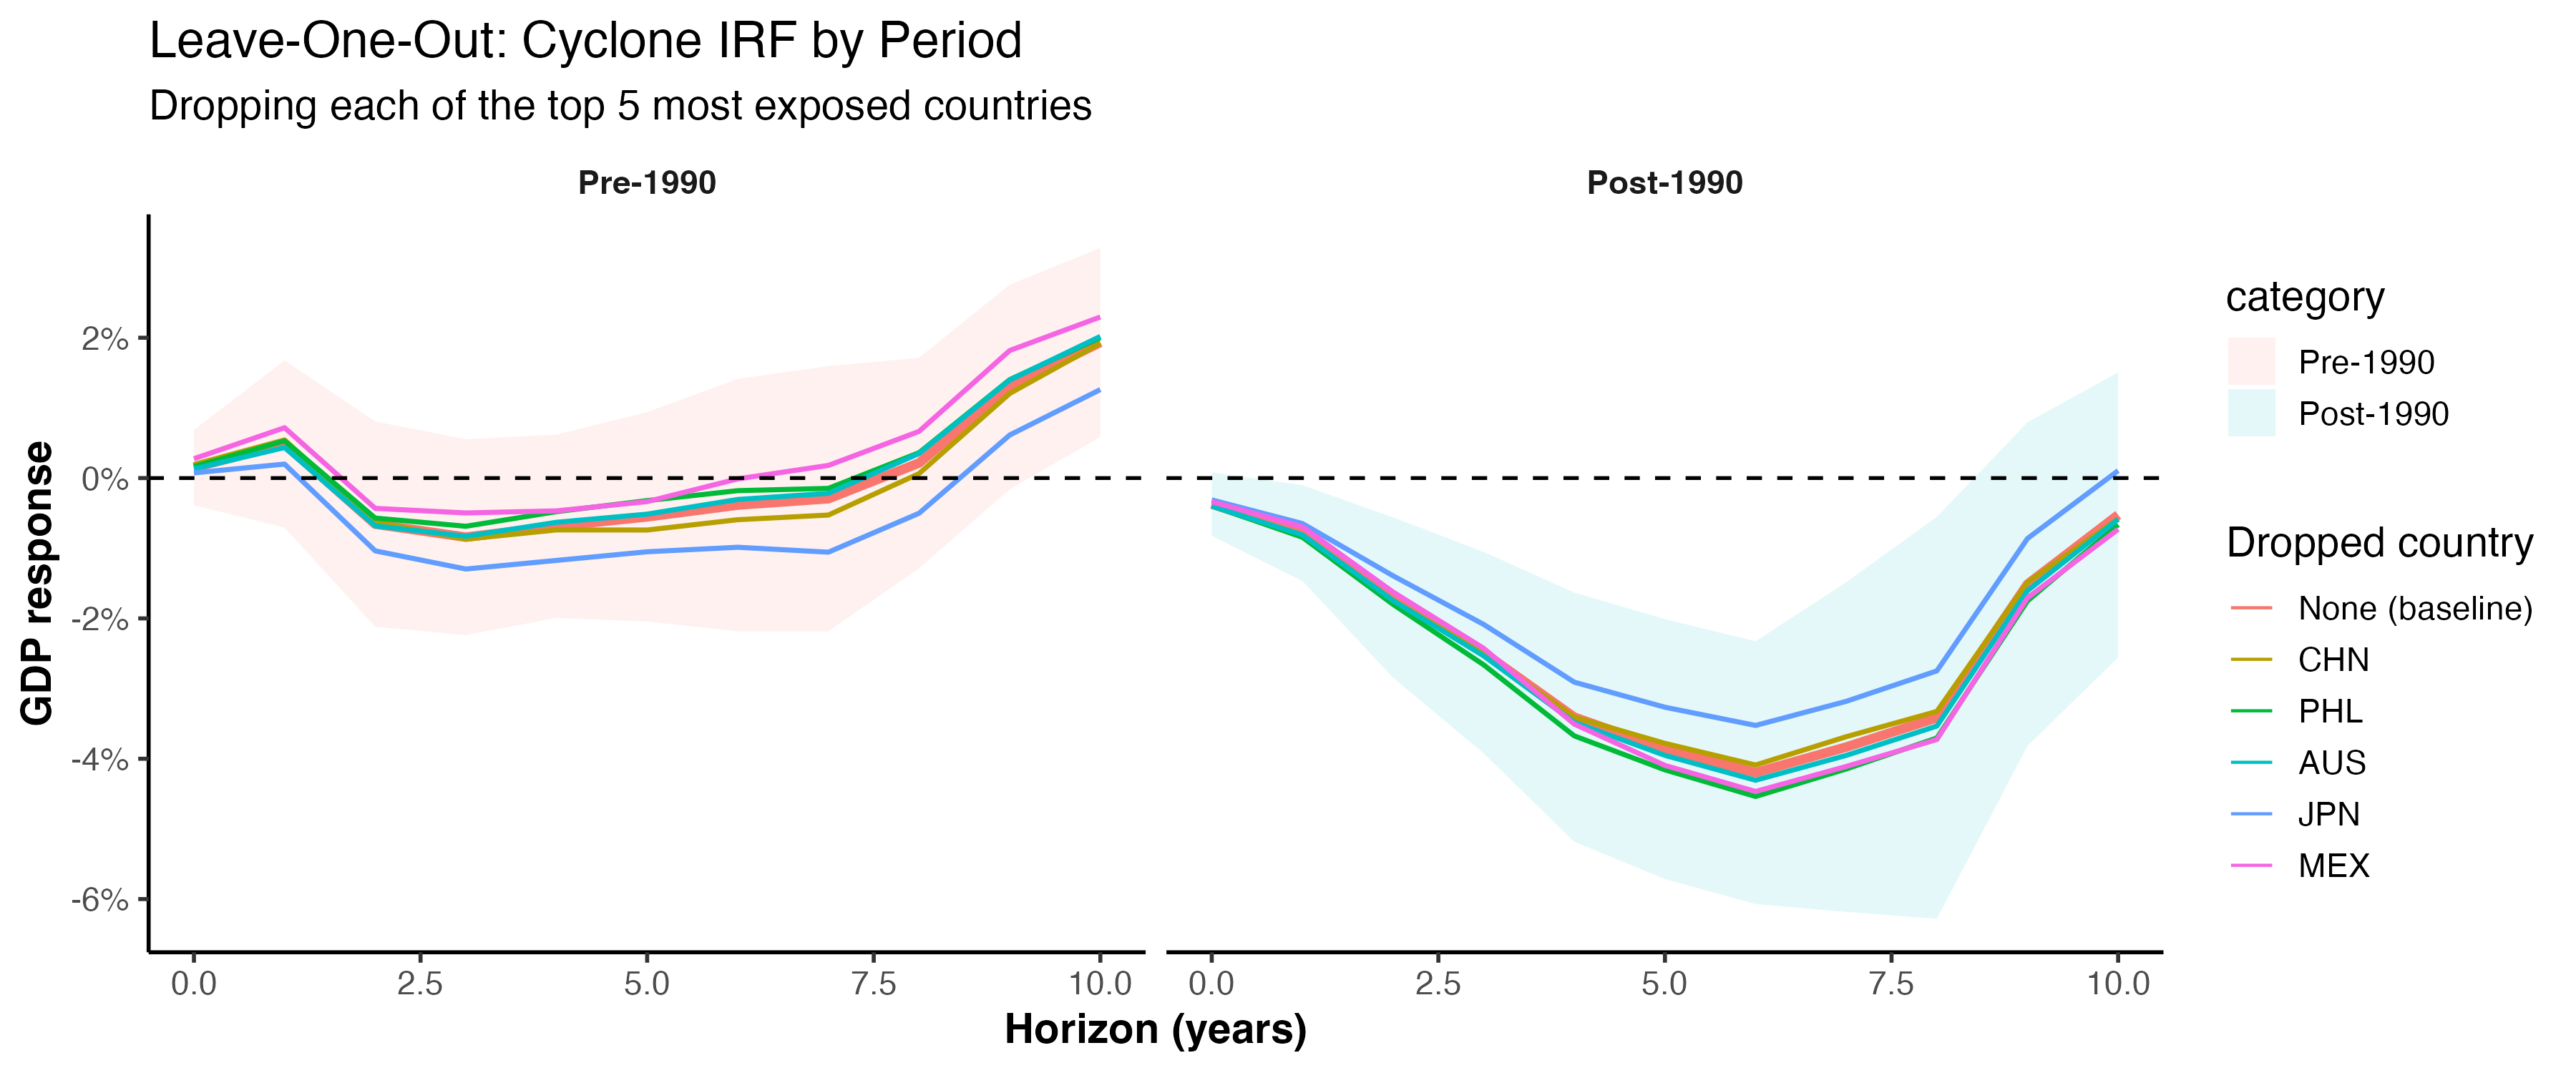
\includegraphics[width=\textwidth,height=0.65\textheight,keepaspectratio]{figures/vulnerability_loo_both_periods.png}

\smallskip
{\small Both periods}
\end{columns}
\end{frame}

\begin{frame}{Robustness Summary}
\begin{itemize}
  \item LOO-year CV: 0.098 --- well below fragility thresholds
  \item LOO-country CV: 0.050 --- very stable
  \item Most influential year: 1998 (Hurricane Mitch, 13 countries)
  \item Most influential countries: JPN, ZWE, VNM, MOZ, VGB
  \item No single observation reverses the sign of the post-1990 effect
\end{itemize}
\bigskip
The post-1990 result is not driven by outliers.
\end{frame}

% ===============================================================
\section*{}
% ===============================================================

\begin{frame}{Conclusion}
\begin{enumerate}
  \item Cyclone shocks reduce GDP per capita by \textbf{2--4\%} over 5--10 years
  \medskip
  \item The apparent post-1990 worsening is largely a \textbf{control group artifact}:
  \begin{itemize}
    \item 142/182 countries never experience cyclone shocks
    \item They are concentrated in Europe and Africa; treated countries in the Americas and Asia
    \item With \textbf{region$\times$year FE}, the pre/post divergence disappears
  \end{itemize}
  \medskip
  \item The baseline cyclone effect (negative, persistent) is \textbf{robust} to LOO checks and alternative samples
  \medskip
  \item Implication: studies using global panels with TWFE should ensure the control group provides a relevant counterfactual for treated units
\end{enumerate}
\end{frame}

\end{document}
